% exercises.tex

% 
\PassOptionsToPackage{noanswers}{camnotes}
%\PassOptionsToPackage{blankanswers}{camnotes}

% uncomment to set draft option for graphicx (already included in camnotes.sty)
%\PassOptionsToPackage{draft}{graphicx}

% uncomment to typeset exercises individually
%\includeonly{ex0_source}
%\includeonly{ex1_source}
%\includeonly{ex2_source}
%\includeonly{ex3_source}
%\includeonly{ex4_source}
%\includeonly{ex5_source}

% These options/settings can be automated using a script:
% $echo "\includeonly{ex0_source}% exercises.tex

% uncomment to set options for camnotes
\PassOptionsToPackage{noanswers}{camnotes}
%\PassOptionsToPackage{blankanswers}{camnotes}

% uncomment to set draft option for graphicx (already included in camnotes.sty)
%\PassOptionsToPackage{draft}{graphicx}

% uncomment to typeset exercises individually
%\includeonly{ex0_source}
%\includeonly{ex1_source}
%\includeonly{ex2_source}
%\includeonly{ex3_source}
%\includeonly{ex4_source}
%\includeonly{ex5_source}

% These options/settings can be automated using a script:
% $echo "\includeonly{ex0_source}% exercises.tex

% uncomment to set options for camnotes
\PassOptionsToPackage{noanswers}{camnotes}
%\PassOptionsToPackage{blankanswers}{camnotes}

% uncomment to set draft option for graphicx (already included in camnotes.sty)
%\PassOptionsToPackage{draft}{graphicx}

% uncomment to typeset exercises individually
%\includeonly{ex0_source}
%\includeonly{ex1_source}
%\includeonly{ex2_source}
%\includeonly{ex3_source}
%\includeonly{ex4_source}
%\includeonly{ex5_source}

% These options/settings can be automated using a script:
% $echo "\includeonly{ex0_source}% exercises.tex

% uncomment to set options for camnotes
\PassOptionsToPackage{noanswers}{camnotes}
%\PassOptionsToPackage{blankanswers}{camnotes}

% uncomment to set draft option for graphicx (already included in camnotes.sty)
%\PassOptionsToPackage{draft}{graphicx}

% uncomment to typeset exercises individually
%\includeonly{ex0_source}
%\includeonly{ex1_source}
%\includeonly{ex2_source}
%\includeonly{ex3_source}
%\includeonly{ex4_source}
%\includeonly{ex5_source}

% These options/settings can be automated using a script:
% $echo "\includeonly{ex0_source}\input{exercises.tex}" > main.tex
% $pdflatex main.tex
% 

% document class
\documentclass[oneside, 11pt]{article}

\usepackage{amsthm}
\usepackage[cm]{fullpage}

\usepackage[margin=30mm]{geometry}

\usepackage{camnotes}
\answercolour{blue}

% module info
%\modulecode{MA2003}
%\moduletitle{Complex Analysis I}
%\academicyear{2017-18}

%\renewcommand{\thetheorem}{\arabic{chapter}.\arabic{theorem}}
% load packages
\usepackage{amsmath}
\usepackage{comment}
\usepackage{verbatim}
\usepackage{mathtools}
\usepackage{amsfonts}
\usepackage{amssymb}
\usepackage{wrapfig}
\usepackage{setspace}

\usepackage{framed}
\usepackage{enumitem}
\usepackage{array}
\usepackage{xcolor}
\usepackage{float}
\usepackage[mode=buildnew]{standalone}% requires -shell-escape
\usepackage{sidecap}
\usepackage{version}
\usepackage{todonotes}
\sidecaptionvpos{figure}{r}
\renewcommand\sidecaptionsep{2cm}

\setstretchfactor{1.5} 
\setimagestretchfactor{1}
\setboxrule{0.5pt}

% document info
\title{Exercise Sheets}
\author{D McConnell}
\date{Summer 2017}

\graphicspath{{./images/}}

% new commands
\newcommand{\contint}{\int_{\mathcal{C}}}
\newcommand{\conj}[1]{\overline{#1}}
\newcommand{\conjugate}[1]{\overline{#1}}
\renewcommand{\Re}{\textsf{Re}}
\renewcommand{\Im}{\textsf{Im}}
\newcommand{\abs}[1]{\left| #1 \right|}
\newcommand{\set}[1]{\left\{#1\right\}}
\newcommand{\brac}[1]{\left( #1 \right) }
\newcommand{\pd}[2]{\dfrac{\partial #1}{\partial #2}}
\newcommand{\rlim}[2]{\lim_{\substack{#1, \\ #2}}}
\newcommand{\reverse}[1]{\widetilde{#1}}
\newcommand{\id}{\textsf{id}}
\newcommand{\Res}{\mathrm{Res}}
\newcommand{\Arg}{\mathrm{Arg}}
\newcommand{\polar}[2]{#1 \left( \cos \left( #2 \right) + i \sin \left( #2 \right) \right)}
\newcommand{\expform}[2]{ #1 \exp \left( #2 \right)}
\newcommand{\R}{\mathbb{R}}
\newcommand{\C}{\mathbb{C}}
\newcommand{\cont}{\mathcal{C}}
\newcommand{\less}[1]{\backslash \set{#1}}

\DeclareMathOperator{\Log}{Log}

\newcommand{\leftimage}[2]{
\begin{tabular}{c@{\hskip 1cm} m{0.5\textwidth} }
\begin{minipage}{0.5\textwidth}
\begin{center}
\begingroup
#1
\endgroup
\end{center}
\end{minipage}
&
\blankson\begingroup
#2
\endgroup\blanksoff
\end{tabular}
}

\newcommand{\exercisetitle}[1]{\begin{center}{\large\bf MA2003 Complex Analysis \\#1}\end{center}\bigskip}

%\includeonly{ex1_source}

\begin{document}
\include{ex0_source}
\setcounter{page}{1}
\include{ex1_source}
\setcounter{page}{1}
\include{ex2_source}
\setcounter{page}{1}
\include{ex3_source}
\setcounter{page}{1}
\include{ex4_source}
\setcounter{page}{1}
\include{ex5_source}
\setcounter{page}{1}
\end{document}" > main.tex
% $pdflatex main.tex
% 

% document class
\documentclass[oneside, 11pt]{article}

\usepackage{amsthm}
\usepackage[cm]{fullpage}

\usepackage[margin=30mm]{geometry}

\usepackage{camnotes}
\answercolour{blue}

% module info
%\modulecode{MA2003}
%\moduletitle{Complex Analysis I}
%\academicyear{2017-18}

%\renewcommand{\thetheorem}{\arabic{chapter}.\arabic{theorem}}
% load packages
\usepackage{amsmath}
\usepackage{comment}
\usepackage{verbatim}
\usepackage{mathtools}
\usepackage{amsfonts}
\usepackage{amssymb}
\usepackage{wrapfig}
\usepackage{setspace}

\usepackage{framed}
\usepackage{enumitem}
\usepackage{array}
\usepackage{xcolor}
\usepackage{float}
\usepackage[mode=buildnew]{standalone}% requires -shell-escape
\usepackage{sidecap}
\usepackage{version}
\usepackage{todonotes}
\sidecaptionvpos{figure}{r}
\renewcommand\sidecaptionsep{2cm}

\setstretchfactor{1.5} 
\setimagestretchfactor{1}
\setboxrule{0.5pt}

% document info
\title{Exercise Sheets}
\author{D McConnell}
\date{Summer 2017}

\graphicspath{{./images/}}

% new commands
\newcommand{\contint}{\int_{\mathcal{C}}}
\newcommand{\conj}[1]{\overline{#1}}
\newcommand{\conjugate}[1]{\overline{#1}}
\renewcommand{\Re}{\textsf{Re}}
\renewcommand{\Im}{\textsf{Im}}
\newcommand{\abs}[1]{\left| #1 \right|}
\newcommand{\set}[1]{\left\{#1\right\}}
\newcommand{\brac}[1]{\left( #1 \right) }
\newcommand{\pd}[2]{\dfrac{\partial #1}{\partial #2}}
\newcommand{\rlim}[2]{\lim_{\substack{#1, \\ #2}}}
\newcommand{\reverse}[1]{\widetilde{#1}}
\newcommand{\id}{\textsf{id}}
\newcommand{\Res}{\mathrm{Res}}
\newcommand{\Arg}{\mathrm{Arg}}
\newcommand{\polar}[2]{#1 \left( \cos \left( #2 \right) + i \sin \left( #2 \right) \right)}
\newcommand{\expform}[2]{ #1 \exp \left( #2 \right)}
\newcommand{\R}{\mathbb{R}}
\newcommand{\C}{\mathbb{C}}
\newcommand{\cont}{\mathcal{C}}
\newcommand{\less}[1]{\backslash \set{#1}}

\DeclareMathOperator{\Log}{Log}

\newcommand{\leftimage}[2]{
\begin{tabular}{c@{\hskip 1cm} m{0.5\textwidth} }
\begin{minipage}{0.5\textwidth}
\begin{center}
\begingroup
#1
\endgroup
\end{center}
\end{minipage}
&
\blankson\begingroup
#2
\endgroup\blanksoff
\end{tabular}
}

\newcommand{\exercisetitle}[1]{\begin{center}{\large\bf MA2003 Complex Analysis \\#1}\end{center}\bigskip}

%\includeonly{ex1_source}

\begin{document}
% !TEX root = exercises.tex

\exercisetitle{Exercise Sheet 0}

\begin{questions}
\question Write the following complex numbers in polar form $z=r \left( \cos ( \theta)+ i \sin (\theta) \right)$ (or equivalently, $z=r \exp \left(i \theta \right)$):
\begin{parts}
\part $1+i$
\part $-1+i$
\part $1+i \sqrt{3}$
\part $\dfrac{(1+i)^7}{(1+i\sqrt{3})^2}$
\end{parts}

\begin{answer}
\begin{enumerate}
\item[(a)] $1+i=\sqrt{2} \left( \cos ( \frac{\pi}{4} ) + i \sin ( \frac{\pi}{4} ) \right)$
\item[(b)] $-1+i=\sqrt{2} \left( \cos ( \frac{3\pi}{4} ) + i \sin ( \frac{3\pi}{4} ) \right)$
\item[(c)] $1+i\sqrt{3}=2 \left( \cos ( \frac{\pi}{3} ) + i \sin ( \frac{\pi}{3} ) \right)$
\item[(d)] While we could expand the numerator and denominator and then simplify, it is much easier to use De Moivre's Theorem:
\[
r \left( \cos ( \theta) + i \sin (\theta ) \right)^n = r^n \left( \cos ( n\theta) + i \sin ( n \theta ) \right) \quad (n \in \mathbb{Z}).
\]
\begin{align*}
(1+i)^7 & = \polar{2^{7/2}}{7 \pi / 4},\\ 
(1+ i \sqrt{3})^{-2} & = \polar{2^{-2}}{-2\pi/3}.
\end{align*}
Then we get
\begin{align*}
\frac{(1+i)^7}{(1+i\sqrt{3})^2} & = (1+i)^7(1+i \sqrt{3})^{-2} \\
& = \polar{2^{3/2}}{13\pi/12}. 
\end{align*}
This is fine, however, if we wish to use the principal value of the argument, we must subtract an appropriate integer multiple of $2\pi$ from $13\pi/12$ (to ensure that the argument lies in $(-\pi,\pi]$).  This is given by  $13\pi /12-2\pi = -11\pi/12$, thus
\[
\frac{(1+i)^7}{(1+i\sqrt{3})^2} = \polar{2^{3/2}}{-11\pi /12}.
\]
An equally valid way of answering this is using the exponential polar form:
\[
(1+i)^7 = \expform{2^{7/2}}{7 \pi / 4}\qquad(1+ i \sqrt{3})^{-2} = \expform{2^{-2}}{-2\pi/3}.
\]
The properties $\exp(z_1)\exp(z_2)=\exp(z_1+z_2)$ and $\exp(z+2\pi i)=\exp(z)$  give:
\[
\frac{(1+i)^7}{(1+i\sqrt{3})^2} = \expform{2^{7/2}}{7 \pi/4} \expform{2^{-2}}{-2\pi/3}  =  \expform{2^{3/2}}{-11\pi/12}.
\]
\end{enumerate}
\end{answer}

\question 
\begin{parts}
\part For $z=a+ib$, express $z^{-1}$ (i.e, $\dfrac{1}{z}$) in Cartesian form
\part Write down the modulus and Principal Argument of $z^{-1}$ in terms of $\abs{z}$ and $\Arg (z)$.
\end{parts}

\begin{answer}
\begin{enumerate}
\item[(a)] We use the fact that $\displaystyle \frac{1}{z} = \frac{1}{z} \cdot \frac{\conj{z}}{\conj{z}} = \frac{\conj{z}}{\abs{z}^2}$ to invert any nonzero complex number:
\[
\frac{1}{a+ib} = \frac{1}{a+ib} \cdot \frac{a-ib}{a-ib} = \frac{a-ib}{a^2+b^2} = \frac{a}{a^2+b^2} - i\frac{b}{a^2+b^2}.
\]
\item[(b)] Writing $z=\polar{r}{\theta}$, De Moivre's Theorem gives
\[
z^{-1} = \left(\polar{r}{\theta}\right)^{-1} = \polar{\frac{1}{r}}{-\theta}.
\]
Hence $\abs{z^{-1}} = 1/\abs{z}$ and $\Arg (z^{-1})=-\Arg (z)$.
\end{enumerate}
\end{answer}

\question Express the following complex numbers in Cartesian form (that is to say, as $a+ib$ for $a,b \in \R$)
\[
\frac{i-1}{1-i}\qquad \frac{1}{1+i}\qquad \frac{3+4i}{1-2i}.
\]
\begin{answer}
In each case, we make the denominator of the quotient $\frac{z_1}{z_2}$ real by multiplying by $\conj{z_2}/ \conj{z_2}$, which gives
\[
\frac{z_1}{z_2} = \frac{z_1\conj{z_2}}{\abs{z_2}^2}.
\]
Thus for example
\begin{align*}
\frac{i-1}{1-i} & = \frac{i-1}{1-i} \cdot \frac{1+i}{1+i} \\
& = \frac{1}{2} \left[ i(1+i)-1(1+i) \right] \\
& = \frac{1}{2} \left[-2 \right] \\
& = -1\ (+i0).
\end{align*}
Similarly
\begin{align*}
\frac{1}{1+i} &=  \frac{1}{2} - \frac{i}{2} \\
\frac{3+4i}{1-2i} &= -1+2i.
\end{align*}
\end{answer}

\question Find the principal argument of the four points $\pm 1\pm i\sqrt{3}$.
\begin{answer}
\begin{align*}
\Arg (1+i\sqrt{3}) &= \frac{\pi}{3} \\
\Arg (-1+i \sqrt{3} ) &= \frac{2\pi}{3} \\
\Arg (-1-i\sqrt{3} ) &= - \frac{2\pi}{3} \\
\Arg (1-i\sqrt{3} ) &= - \frac{\pi}{3}. 
\end{align*}
\end{answer}




\question Calculate
\[
\Arg \left. \left( \frac{1}{2} + \frac{1}{z^2} \right) \right|_{z=1+i}.
\]
(The notation
$
\left. f(z) \right|_{z=w}
$
means $f(z)$ evaluated at $z=w$, or in other words, $f(w)$.)
\begin{answer}
We have
\[
\frac{1}{2} + \frac{1}{(1+i)^2} = \frac{1}{2}-\frac{i}{2},
\]
with principal argument $-\frac{\pi}{4}$.
\end{answer}
\question Show that
\[
2 \left( \frac{z}{z+i} \right) \left. \frac{(z+i-z)}{(z+i)^2} \right|_{z=i} = \frac{-i}{4}.
\]
\begin{answer}
\begin{align*}
2 \left( \frac{z}{z+i} \right) \left. \frac{(z+i-z)}{(z+i)^2} \right|_{z=i} & = 2 \left( \frac{i}{2i} \right) \left( \frac{i+i-i}{(2i)^2} \right) \\
& = \frac{2i}{2i} \frac{i}{(-4)} = -\frac{i}{4}.
\end{align*}
\end{answer}


\question Sketch the following regions of $\C$:
\begin{parts}
\part $1 < |z| < 2$ (This notation is shorthand for the set $\set{ z \in \C: 1 < \abs{z} <2}$.)
\part $1<|z+2|<2$
\part $1 < \Im (z-i) < 2$
\end{parts}
\begin{answer}

\begin{enumerate}
\item[(a),(b)] Note that for $\alpha \in \C$ and $r>0$, the set $\set{ z \in \C: \abs{z-\alpha} = r}$ is precisely the circle of radius $r$ centred at $\alpha$.  The sets $0<\abs{z-\alpha}<r$ and $\abs{z-\alpha}>r$ respectively are the regions inside and outside the circle.

Hence $1<z<2$ is the region outside the circle of radius 1 centred at 0, and inside the circle of radius 2 centred at 0.  The set $1<\abs{z+2}<2$ is the same but with circles centred at $-2$.  A set of this type is called an \emph{annulus}.
\begin{center}
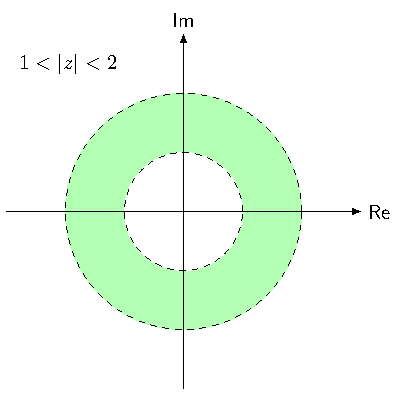
\includegraphics[scale=0.75]{annulus}\quad 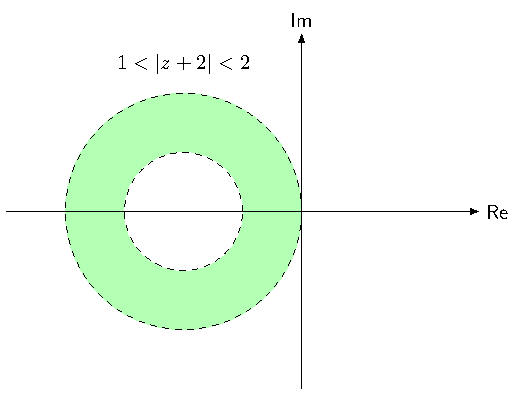
\includegraphics[scale=0.75]{annulus2}
\end{center}

\item[(c)] Write $z=x+iy$, then $z-i = x+i(y-1)$ and so
\begin{align*}
\set{z\in \C: 1 < \Im(z-i) <2 } &= \set{ x+iy \in \C : 1<y-1 <2 } \\
&= \set{x+iy \in \C: 2<y<3},
\end{align*}
which is the infinite horizontal band bounded by the lines $y=2$ and $y=3$.
\begin{center}
\oldincludegraphics[scale=0.75]{band}
\end{center}
\end{enumerate}
\end{answer}
\question 
\begin{parts}
\part Prove that for two nonzero complex numbers $z_1$ and $z_2$ we have
\[
\abs{z_1z_2} = \abs{z_1} \cdot \abs{z_2} \quad\text{ and }\quad \arg(z_1z_2)=\arg(z_1)\arg(z_2)
\]
(hint: write $z_1$ and $z_2$ in polar form).  Is it always true that $\Arg(z_1z_2)=\Arg(z_2)+\Arg(z_2)$?
\begin{answer}
Writing
\[
z_1=\polar{r_1}{\theta_1}\quad\text{and}\quad z_2=\polar{r_2}{\theta_2}
\]
we see that
\begin{align*}
z_1z_2&=r_1r_2 \left( \cos(\theta_1)\cos(\theta_2)-\sin(\theta_1)\sin(\theta_2) +i \left[ \cos(\theta_1)\sin(\theta_2)+\cos(\theta_2)\sin(\theta_1) \right] \right) \\
& = r_1r_2 \left( \cos(\theta_1+\theta_2)+i \sin(\theta_1+\theta_2) \right).
\end{align*}
Thus
\[
\abs{z_1z_2}=r_1r_2=\abs{z_1}\cdot \abs{z_2}\quad\text{and}\quad \arg(z_1z_2)=\theta_1+\theta_2=\arg(z_1)+\arg(z_2).
\]
It is not always true that $\Arg(z_1z_2)=\Arg(z_1)+\Arg(z_2)$.  Indeed, if $z_1=z_2=-1$ we have $\Arg (-1)=\pi$ but
\[
\Arg ((-1)(-1)) = \Arg (1) = 0.
\]
\end{answer}
\part Show that $\exp(z_1)\exp(z_2) = \exp(z_1+z_2)$.
\begin{answer}
With $z_1=x_1+iy_1$ and $z_2=x_2+iy_2$ a similar calculation to part (a) shows that
\begin{align*}
\exp(z_1)\exp(z_2) &= \polar{e^{x_1}}{y_1} \polar{e^{x_2}}{y_2} \\
 & = \polar{e^{x_1}e^{x_2}}{y_1+y_2} \\
 & = \polar{e^{x_1+x_2}}{y_1+y_2} = \exp(z_1+z_2).
\end{align*}
\end{answer}
\end{parts}
\question Write down the $3^{rd}$ roots of $-8$ in Cartesian form.
\begin{answer}
Writing $-8=\polar{8}{\pi}$, the three cubic roots are of the form $\polar{\sqrt[3]{8}}{(\pi+2k\pi)/3}$ for $k=0,1,2$.  In polar form, these are
\[
\polar{2}{\pi/3}, \quad \polar{2}{\pi} \quad\text{and}\quad\polar{2}{5\pi/3},
\]
or in Cartesian form $1+\sqrt{3},\ -2$ and $1-\sqrt{3}$ respectively.

\end{answer}

\question Find the values of $z$ for which $z^2+4iz-1=0$.  Which of these values lies inside the circle $C=\set{z \in \C: \abs{z}=1}$.
\begin{answer}
This is simply the usual quadratic formula: the roots of this polynomial are given by
\[
\frac{-4i\pm \sqrt{(4i)^2-4(1)(-1)}}{2} = \frac{-4i\pm i \sqrt{12}}{2} = i (-2 \pm  \sqrt{3}).
\]
To see which of these lies inside the circle $\abs{z}=1$, we examine the modulus and see that $\abs{i(-2 + \sqrt{3})} \approx 0.071<1$ and $\abs{i(-2-\sqrt{3})} \approx 1.93>1$. Thus only $i(-2+\sqrt{3})$ lies inside this circle.
\end{answer}


\question Show that $\Re (z) \leq \abs{ \Re (z)} \leq \abs{z}$ and $\abs{\Re (z)}+\abs{\Im (z)} \leq \sqrt{2} \abs{z}$.
\begin{answer}
The fact that $\Re (z) \leq \abs{ \Re (z)}$ is trivial.  Moreover,  writing $z=x+iy$ we see that
\[
\abs{\Re(z)} = \sqrt{x^2} \leq \sqrt{x^2+y^2}
\]
since $x^2 \leq x^2+y^2$ (and the square root function is increasing).

For the second inequality, note that with $z=x+iy$,
\begin{align*}
\left( \abs{\Re (z)}+\abs{\Im (z)} \right)^2 & = \left( \abs{x}+\abs{y} \right)^2 \\
& \leq \left( \abs{x}+\abs{y} \right)^2  + \overbrace{\left( \abs{x}-\abs{y} \right)^2}^{\geq 0}  \\
& = x^2+y^2+2\abs{xy} + x^2 + y^2 - 2\abs{xy} \\
& = 2(x^2+y^2) = 2 \abs{z}^2.
\end{align*}
Taking square roots of both sides yields the required inequality.
\end{answer}
\end{questions}

\setcounter{page}{1}
% !TEX root = exercises.tex

\exercisetitle{Exercise Sheet 1}

\begin{questions}
\question Use the triangle inequality $\abs{z_1-z_2} \leq \abs{z_1} + \abs{z_2}$ to prove the reverse triangle inequality:
\[
\abs{z_1-z_2} \geq \abs{\abs{z_1}-\abs{z_2}}
\]
\begin{answer}
The triangle inequality gives
\begin{align*}
\abs{z_1} & = \abs{z_1-z_2+z_2} \leq \abs{z_1-z_2} + \abs{z_2}  \\
\abs{z_2} & = \abs{z_2-z_1+z_1} \leq \abs{z_2-z_1} + \abs{z_1}\ (=\abs{z_1-z_2}+\abs{z_1}).
\end{align*}
Rearranging gives the two inequalities
\begin{align*}
\abs{z_1-z_2} & \geq \abs{z_1} - \abs{z_2} \\
\abs{z_1-z_2} & \geq \abs{z_2} - \abs{z_1},
\end{align*}
or in other words
\[
\abs{z_1-z_2} \geq \max \left( \abs{z_1}-\abs{z_2} , \abs{z_2} - \abs{z_1} \right) = \abs{\abs{z_1} - \abs{z_2} }.
\]
\end{answer}
\question Use the triangle and reverse triangle inequalities to show that for all $z$ on the circle $\abs{z}=2$, we have
\[
\abs{z+2} \leq 4 \text{ and } \abs{z-3+4i} \geq 3.
\]
Describe these inequalities geometrically.
\begin{answer}
If $\abs{z}=2$ then the triangle inequality ensures that
\[
\abs{z+2} \leq \abs{z}+2 = 4,
\]
and the backwards triangle inequality gives
\begin{align*}
\abs{z-3+4i} & = \abs{z-(3-4i)} \\
& \geq \abs{ \abs{z} - \abs{3-4i} } \\
& = \abs{2-5} = 3.
\end{align*}
Geometrically, these inequalities show respectively that the circle $\abs{z}=2$ is
\begin{itemize}
\item Contained in the disc with centre $-2$ and radius $4$ (i.e., the disc $\abs{z+2} \leq 4$), and
\item Outside of the disc with centre $3-4i$ and radius $3$.
\end{itemize}
\begin{center}
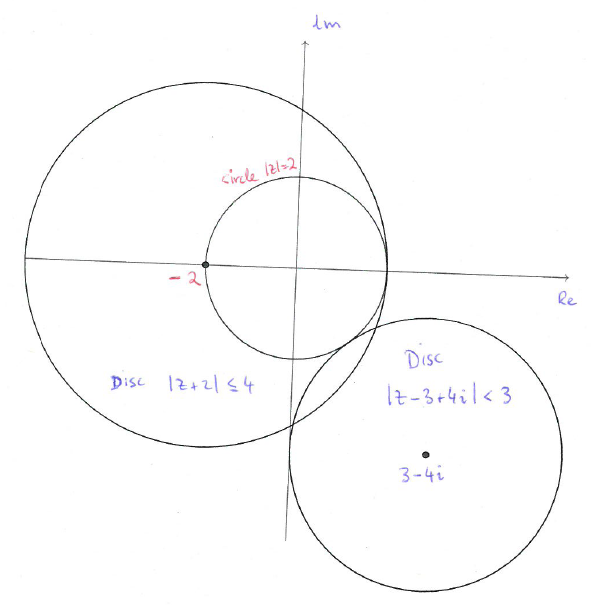
\includegraphics[scale=0.5]{ex1_q2}
\end{center}
\end{answer}
\question Use the triangle and reverse triangle inequalities to show that for all $z$ on the circle $\abs{z+3i}=3$ we have
\[
\abs{z-4} \leq 8,\quad \abs{z+5i}\geq 1 \text{ and } \abs{ \frac{z-4}{z+5i} } \leq 8.
\]
\begin{answer}

As with the previous question, the triangle inequality yields
\begin{align*}
\abs{z-4} & = \abs{z+3i-(3i+4)} \\
& \leq \abs{z+3i} + \abs{3i+4} \\
&=3+5=8.
\end{align*}
and the backwards triangle inequality yields
\begin{align*}
\abs{z+5i} & = \abs{z+3i+2i} \\
& \geq \abs{ \abs{z+3i} - \abs{2i} } \\
&=3-2=1.
\end{align*}
The third inequality is then obvious.
\end{answer}
\question Let $L$ be the line segment $[0,h]$ where $h \in \C$ and $\abs{h} < r$.  Show that if $\beta \in \C$ with $\abs{\beta}>2r$ and $z \in L$ then
\[
\abs{\frac{h-z}{\beta-z}} < \frac{\abs{h}}{r}.
\]
Do this using the reverse triangle inequality.  It can also be seen as follows.  Draw $L$ and two circles, both with centre $0$, $C_1$ with radius $r$ and $C_2$ with radius $2r$.  Why does $L$ lie inside $C_1$?  Where is $\beta$ on your diagram?  Why is $\abs{\beta-z}>r$?  If you can answer these three questions then the inequality should follow easily.
\begin{answer}

\begin{center}
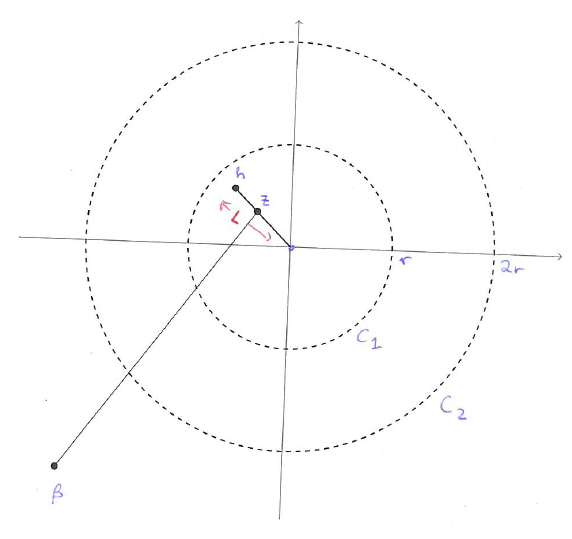
\includegraphics[scale=0.7]{ex1_q3}
\end{center}
Since $z$ lies on $L$, it is clear that $\abs{h-z} \leq \abs{h}$ (more formally, we can write $z=th$ for some $t$ with $0 \leq t \leq 1$, so that $\abs{h-z} = \abs{(1-t)h} = (1-t) \abs{h} \leq \abs{h}$).

The backwards triangle inequality, together with the fact that $\abs{z}<r<2r<\abs{\beta}$ gives
\begin{align*}
\abs{\beta - z} & \geq \abs{\abs{\beta}-\abs{z}} \\
& = \abs{\beta} - \abs{z} \\
&> 2r-r = r.
\end{align*}

Combining these two inequalities we see that
\begin{align*}
\abs{ \frac{h-z}{\beta - z} } &= \frac{\abs{h-z}}{\abs{\beta -z}} \\
 & \leq \frac{\abs{h}}{\abs{\beta - z}} \\
 & < \frac{\abs{h}}{r}.
\end{align*}

\end{answer}
\question The function $\mathbf{f}: \R^2 \to \R^2$ is defined by
$
\mathbf{f} (x,y)=(0,2y).
$
Show that the corresponding complex function $f:\C \to \C$ is
$
f(z) = z- \conj{z},
$
and that
\[
\lim_{h \to 0} \frac{f(z_0+h)-f(z_0)}{h}
\]
does not exist at any point $z_0 \in \C$.
\begin{answer}
The corresponding function is
\[
f(z) = f(x+iy) = i(2y) = i ( 2 \Im (z) ) = 2i \cdot \frac{z-\conj{z}}{2i} = z - \conj{z}.
\]
If $z_0 \in \C$ and $h \in \C \backslash \set{0}$ then
\[
\frac{f(z_0+h)-f(z_0)}{h} = \frac{(z_0+h)-\conj{(z_0+h)} - (z-\conj{z})}{h} = \frac{h-\conj{h}}{h} = 1- \frac{\conj{h}}{h}.
\]
Looking at restricted limits along the real and imaginary axes:
\[
1-\frac{\conj{h}}{h} \to \begin{cases}
1-1=0 & \text{ as } h \to 0, h \in \mathbb{R} \\
1-(-1)=2 & \text{ as } h \to 0, h \in i \R.
\end{cases}
\]
Since the restricted limits are not equal the (unrestricted) limit does not exist for any $z_0 \in \C$.

\end{answer}
\question Same as question 5 but with
\[
\mathbf{f}(x,y)=(x^2-y^2-x,2xy+y+1) \quad\text{ and }\quad f(z)=z^2-\conj{z}+i.
\]
\begin{answer}
This time, it is easier to start with the complex function $f$ and substitute $z=x+iy$:
\begin{align*}
f(z) & = z^2-\conj{z} + i \\
& = (x+iy)^2-(x-iy)+i \\
& = x^2-y^2+i2xy -x +iy +i \\
& = x^2-y^2-x + i \left( 2xy+y+1 \right),
\end{align*}
which shows that $f$ corresponds to the function $\mathbf{f}:\R^2 \to \R^2$ where
\[
\mathbf{f} (x,y) = \left( x^2-y^2-x, 2xy+y+1 \right).
\]
For $z_0 \in \C$ and $h \in \C \backslash \set{0}$ the difference quotient is
\begin{align*}
\frac{f(z_0+h)-f(z_0)}{h} & = \frac{(z_0+h)^2-\conj{(z_0+h)}+i-(z_0^2-\conj{z_0}+i )}{h} \\
& = h+2z_0-\frac{\conj{h}}{h}.
\end{align*}
Looking at some restricted limits:
\begin{align*}
\rlim{h \to 0}{h \in \R \backslash \set{0}} \frac{f(z_0+h)-f(z_0)}{h} & = 2z_0-1 \\
\rlim{h \to 0}{h \in i\R \backslash \set{0}} \frac{f(z_0+h)-f(z_0)}{h} & = 2z_0+1. \\
\end{align*}
These are not equal for any $z_0 \in \C$, so the unrestricted limit
\[
\lim_{h \to 0} \frac{f(z_0+h)-f(z_0)}{h}
\]
does not exist at any $z_0 \in \C$. 
\end{answer}
\question Let $f:\C \to \C$ be defined by $f(z) = \abs{z}^2$.  Show that $f$ is differentiable at $z=0$ and nowhere else.
\begin{answer}
Since $\abs{z}^2 = z \conj{z}$,
\begin{align*}
\frac{f(z_0+h)-f(z_0)}{h} &= \frac{(z_0+h)\conj{(z_0+h)}-z_0\conj{z_0}}{h} \\
& = \frac{z_0\conj{h}+h\conj{z_0}+h\conj{h}}{h} \\
&= z_0\frac{\conj{h}}{h} + \conj{z_0}+\conj{h} \\
& \longrightarrow
\begin{cases}
2z_0 & \text{ as }h \to 0,\ h \in \R \backslash \set{0} \\
0 & \text{ as } h \to 0, h \in i\R \backslash \set{0}.
\end{cases}
\end{align*}
For $z_0 \neq 0$, the restricted limits are not equal, hence the unrestricted limit does not exist and so $f$ is not differentiable at any point $z_0 \in \C \backslash \set{0}$.

At $z_0=0$, we have
\[
\lim_{h \to 0} \frac{f(0+h)-f(0)}{h} = \lim_{h \to 0} \conj{h} = 0,
\]
so that $f$ is differentiable at $0$ with $f'(0)=0$.
\end{answer}
\question Use the rules of differentiation to find the derivatives of the following functions:
\begin{parts}
\part $f(z) = \left( z^2+4 \right)^3$
\part $g(z) = \dfrac{z+i}{z-i}$.
\end{parts}
Find the values of $f'(i)$ and $g'(1)$.
\begin{answer}
\begin{parts}
\part Since $f$ is the composition of holomorphic functions, we can use the chain rule to find $f'(z)$:
\[
f'(z) = 3 ( z^2+4)^2(2z) = 6z(z^2+4)^2 \quad \text{ for all } z \in \C,
\]
and
\[
f'(i) = 6i (i^2+4)^2 = 6i(3)^2 = 54i.
\]
\part Since the functions $z \mapsto z\pm i$ are holomorphic on $\C$, $g$ is holomorphic on $\C \backslash \set{i}$, and the quotient rule gives
\[
g'(z) = \frac{(z-i)(1)-(z+i)(1)}{(z-i)^2} = \frac{-2i}{(z-i)^2}
\]
for all $z \in \C \backslash \set{i}$.  Hence
\[
g'(1) = \frac{-2i}{(1-i)^2} = \frac{-2i}{-2i} = 1.
\]
\end{parts}
\end{answer}

\end{questions}

\setcounter{page}{1}
% !TEX root = exercises.tex

\exercisetitle{Exercise Sheet 2}

\begin{questions}
\question For each function $f$ below, write $f$ in the form
\[
f(z) = f(x+iy) = u(x,y)+iv(x,y)
\]
and determine whether or not the Cauchy-Riemann equations are satisfied:
\[ (a)\ f(z) = \exp(i\ \conj{z})\quad  (b)\ f(z) = z + \dfrac{1}{z}\quad (c)\ f(z)=z^3.\]

In the cases where $f$ is differentiable, find the derivative of $f$ both using the rules of differentiation and using the Cauchy-Riemann equations.
\begin{answer}
\begin{parts}
\part We have 
\[
f(x+iy) = \exp (i (x-iy) ) = \exp (y+ix ) = \underbrace{e^{y} \cos (x) }_{u(x,y)} + i \underbrace{e^{y} \sin (x)}_{v(x,y)}.
\]
The corresponding partial derivatives are
\begin{align*}
\pd{u}{x} & = -e^{y} \sin(x) & \pd{v}{y} = e^{y} \sin(x) \\
\pd{u}{y} & = e^{y} \cos (x) &  \pd{v}{x} = e^{y} \cos (x).
\end{align*}
The Cauchy Riemann Equations are satisfied at a point $x+iy \in \C$ if and only if both
\[
e^y \sin(x) = -e^{y} \sin(x)\quad\text{and}\quad e^{y} \cos (x) = - e^{y} \cos (x).
\]
Since $e^y$ is never zero, this can only occur if $\sin(x)=\cos(x)=0$, which is impossible.  

\part For all $x +iy \in \C \backslash \set{0}$, 
\begin{align*}
f(x+iy) &= (x+iy) + \frac{1}{x+iy} \\
& = (x+iy) + \frac{x-iy}{x^2+y^2} \\
& = \underbrace{\left( x+ \frac{x}{x^2+y^2}  \right)}_{u(x,y)} + i \underbrace{\left( y-\frac{y}{x^2+y^2} \right) }_{v(x,y)}
\end{align*}
and the corresponding partial derivatives are
\begin{align*}
& \pd{u}{x} = 1+\frac{y^2-x^2}{(x^2+y^2)^2} && \pd{u}{y} = \frac{-2xy}{(x^2+y^2)^2} \\
& \pd{v}{x} = \frac{2xy}{(x^2+y^2)^2} && \pd{v}{y} = 1 - \frac{x^2-y^2}{(x^2+y^2)^2}.
\end{align*}
Hence the Cauchy Riemann equations are satisfied at every $x+iy \in \C \backslash \set{0}$.  Using the Cauchy Riemann equations to find the derivative of $f$, we get
\begin{align*}
f'(x+iy ) & = \pd{u}{x} + i \pd{v}{x} \\
& = \left( 1+\frac{y^2-x^2}{(x^2+y^2)^2} \right) + i \left( \frac{2xy}{(x^2+y^2)^2} \right) \\
& = 1 + \frac{y^2-x^2+i2xy}{(x^2+y^2)^2} \\
& = 1 - \frac{x^2-y^2-i2xy}{(x^2+y^2)^2} \\
& = 1 - \frac{(x-iy)^2}{\left[ (x+iy)(x-iy) \right]^2} \\
& = 1 - \frac{1}{(x+iy)^2} = 1- \frac{1}{z^2},
\end{align*}
which agrees with the derivative of $f$ obtained from the rules of differentiation.
\part This time
\[
u(x,y) = x^3-3xy^2 \quad\text{and}\quad v(x,y)=3x^2y-y^3
\]
hence for all $x+iy \in \C$
\[
\pd{u}{x} = 3x^2-3y^2=\pd{v}{y} \quad\text{and}\quad \pd{u}{y}=-6xy=-\pd{v}{x}.
\]
Thus
\[
f'(x+iy) = \pd{u}{x} (x,y)+i\pd{v}{y}(x,y) = 3x^2-3y^2+i(6xy) = 3 \left( (x^2-y^2)+i(2xy) \right) = 3(x+iy)^2
\]
which agrees with the derivative obtained from the Chain Rule: $f'(z)=3z^2$.
\end{parts}
\end{answer}

\question Show that the Cauchy-Riemann equations are satisfied by the function $f$ defined on the open upper half plane $H_+=\set{ z \in \C: \Im (z) > 0 }$ by
\[
f(x+iy) = u(x,y)+iv(x,y) = \log \left( \sqrt{ x^2+y^2 } \right) + i \left( \frac{\pi}{2} - \arctan \left( \frac{x}{y} \right) \right).
\]
Assuming that $f$ is indeed holomorphic on $H_+$, show that
\[
f'(x+iy) = \frac{1}{x+iy}\quad \text{i.e., that }\quad f'(z) = \frac{1}{z}.
\]
\begin{answer}
We have
\begin{align*}
\pd{u}{x} &= \log' \left( \sqrt{ x^2+y^2 } \right) \cdot \pd{}{x} \left[ \sqrt{x^2+y^2} \right] \\
& = \frac{1}{\sqrt{x^2+y^2}} \cdot \frac{1}{2} (x^2+y^2)^{-\frac{1}{2}}(2x) \\
&=  \frac{x}{x^2+y^2}
\shortintertext{ and similarly }
\pd{u}{y} & = \frac{y}{x^2+y^2}.\\
\intertext{For the partial derivatives of $v$, we have}
\pd{v}{x} & = - \arctan ' \left( \frac{x}{y} \right) \cdot \pd{}{x} \left[ \frac{x}{y} \right] \\
& = \frac{-1}{(1+(\frac{x}{y})^2)} \cdot \frac{1}{y} \\
& = \frac{-1}{y+\frac{x^2}{y}} = \frac{-y}{x^2+y^2} \\
\shortintertext{and }
\pd{v}{y} & = - \arctan ' \left( \frac{x}{y} \right) \cdot \pd{}{y} \left[ \frac{x}{y} \right] \\
& = \frac{-1}{(1+(\frac{x}{y})^2} \cdot \frac{-x}{y^2} \\
& = \frac{x}{x^2+y^2}.
\end{align*}
Thus the Cauchy-Riemann equations 
\[
\pd{u}{x} = \pd{v}{y},\quad \pd{u}{y} = - \pd{v}{x}
\]
are satisfied everywhere in $H_+$.  Assuming moreover that $f$ is holomorphic on $H_+$, the derivative of $f$ is thus
\begin{align*}
f'(x+iy) & = \pd{u}{x} + i \pd{v}{x} \\
& = \frac{x}{x^2+y^2}+i \frac{-y}{x^2+y^2} \\
& = \frac{x-iy}{(x+iy)(x-iy)} = \frac{1}{x+iy}
\end{align*}
for all $x+iy \in H_+$ as required.
\end{answer}

\question Describe the geometric effect of applying the functions:
\begin{parts}
\part $f(z) = \dfrac{1}{z}$ to a small disc centred at $1-i$, and 
\part $g(z) = \exp(2iz)$ to a small disc centred at $\frac{\pi}{4}+i$.
\end{parts}
\begin{answer}
For a function $f$ that is holomorphic at a point $z_0$, we know that a small disc centred at $z_0$ is approximately mapped to a small disc centred at $f(z_0)$, and is scaled by a factor of $\abs{f'(z_0)}$ and rotated by an angle of $\arg (f'(z_0))$ about the point $f(z_0)$.
\begin{parts}
\part In this example, $f(1-i)=\dfrac{1}{1-i}=\dfrac{1}{2}+\dfrac{i}{2}$, so a small disc centred at $1-i$ is approximately mapped to a small disc centred at $\dfrac{1}{2}+\dfrac{i}{2}$.  Since $f'(z) = -\dfrac{1}{z^2}$ for all $z \in \C \backslash \set{0}$, we have $f'(i)=-\dfrac{1}{(1-i)^2} = \frac{i}{2}$.  Thus the disc is scaled by a factor of $\frac{1}{2}$ and rotated by an angle of $\frac{\pi}{2}$ about $\dfrac{1}{2}-\dfrac{i}{2}$.
\part Mapped to a disc centred at $g(\frac{\pi}{4}+i)=e^{-2}i$, scaled by a factor of $2e^{-2}$ and rotated by an angle of $\pi$ about this point (clockwise or anticlockwise; it doesn't matter this time).
\end{parts}
\end{answer}
\question  The \emph{set} of points $L=[0,1-2i]$ is a line segment.  It is also a \emph{path} because we have a parametrisation given by  $\gamma:[0,1] \to \C,\ \gamma(t) = (1-2i)t.$  Use this parametrisation to evaluate the integral
\[
\int_L \left( \Im (z) + 3i \right)\ dz.
\]
\begin{answer}

We have
\begin{align*}
\int_{\Gamma} ( \Im (z) + 3i )\ dz & = \int_0^1 \left( \Im ( \gamma (t) ) +3i \right) \gamma' (t)\ dt \\
& = \int_0^1 \left( -2t + 3i \right) (1-2i)\ dt \\
& = (1-2i) \int_0^1 (-2t +3i)\ dt \\
& = (1-2i) \left[ - t^2 +3it \right]_0^1 \\
& = (1-2i)(-1+3i) = 5 + 5i.
\end{align*}

\end{answer}
\question Find the value of
\[
\int_{\Gamma_1} f(z)\ dz \text{ and } \int_{\Gamma_2} f(z)\ dz,
\]
where $f(z) = 3 \conj{z}$, $\Gamma_1$ is the straight line path from $0$ to $-i$ and $\Gamma_2$ is the straight line path from $1-i$ to $1+i$.
\begin{answer}
For the path $\Gamma_1$ we use the parametrisation $\gamma_1:[0,1] \to \C$, $\gamma_1 (t) = -it.$  Then $\gamma_1'(t)=-i$ and $f(\gamma_1(t)) = 3it$.  Hence
\[
\int_{\Gamma_1} f = \int_0^1 (3it)(-i)dt = \int_0^1 3t\ dt = \frac{3}{2}.
\]
Parametrise $\Gamma_2$ with $\gamma_2:[0,1] \to \C$, where
\[
\gamma_2 (t) = (1-i) + t \left[ 1+i-(1-i) \right] = 1+i(2t-1).
\]
We get
\[
\int_{\Gamma_2} f = 6i.
\]
\end{answer}





\question Fix a point $z_0 \in \C$ and define a complex function $f$ via
\[
f(z) = (z-z_0)^n
\]
where $n \in \mathbb{Z}$.  Find the value of
\[
\int_{\Gamma} f(z)\ dz,
\]
where $\Gamma$ is the circle with centre $z_0$ and radius $r>0$, traversed in the anticlockwise direction (use the parametrisation $\gamma:[0,2\pi] \to \C, \ \gamma (t) = z_0 + r \left( \cos (t) + i \sin (t) \right)$).  Do this separately for the cases $n=-1$ and $n \neq -1$.

(Hint: for the case $n \neq -1$, you need to show that
\[
\frac{d}{dt} \left[ \left( \cos(t)+i \sin(t) \right)^{n+1} \right] = i(n+1) \left( \cos(t)+i \sin(t) \right)^{n+1}
\]
and then use the (real) Fundamental Theorem of Calculus).
\begin{answer}
Following the hint, we first note that
\begin{align*}
\frac{d}{dt} \left[ \left( \cos(t)+i \sin(t) \right)^{n+1} \right] & = (n+1) \left( \cos(t)+i \sin(t) \right)^{n} \left( - \sin (t)+i \cos(t) \right) \\
& = (n+1) \left( \cos(t)+i \sin(t) \right)^{n} i \left( \cos(t)+i \sin(t) \right) \\
& = i(n+1) \left( \cos(t)+i \sin(t) \right)^{n+1}.
\end{align*}
We have
\[
f(\gamma(t))=\left( \gamma(t)-z_0 \right)^n = r^n \left( \cos (t)+i \sin (t) \right)^n,\quad \gamma'(t) = i r\left( \cos(t) + i \sin (t) \right).
\]
Hence for $n \neq -1$,
\begin{align*}
\int_{\Gamma} (z-z_0)^n & = \int_0^{2\pi} i r^{n+1} \left( \cos(t) + i \sin (t) \right)^{n+1}\ dt &&\\
& = \frac{r^{n+1}}{n+1} \int_0^{2\pi} \frac{d}{dt} \left[ \left( \cos(t) + i \sin (t) \right)^{n+1} \right]\ dt && \\
& = \frac{r^{n+1}}{n+1} \left[ \left( \cos(t) + i \sin (t) \right)^{n+1} \right]_0^{2\pi} && \text{ by FTC }\\
& = \frac{r^{n+1}}{n+1} \left[ 1+0i-(1+0i) \right] = 0 &&.
\end{align*}
If $n=-1$ then
\[
\int_{\Gamma} (z- z_0)^{-1} = \int_0^{2\pi} \frac{1}{r(\cos(t)+i\sin(t) )} \cdot ir (\cos(t)+i\sin(t) )\ dt =  \int_0^{2\pi} i\ dt = i2\pi.
\]


\end{answer}
\question Let $f,g:U \to \C$ be continuous, and let $\Gamma$ be a smooth path contained in $U$ parametrised by $\gamma:[a,b] \to \C$.  Prove that
\begin{parts}
\part for every constant $\alpha \in \C$ we have $\displaystyle \int_{\Gamma} ( f + \alpha g ) = \int_{\Gamma} f + \alpha \int_{\Gamma} g$, and
\part if $\tilde{\Gamma}$ denotes the reverse of $\Gamma$, we have $\displaystyle \int_{\tilde{\Gamma}} f = - \int_{\Gamma} f$.  As a hint, parametrise $\tilde{\Gamma}$ using $\tilde{\gamma}:[a,b] \to \C$, $\tilde{\gamma}(t)=(a+b-t)$, and use the substitution $s=a+b-t$.
\end{parts}
\begin{answer}
\begin{parts}
\part 
\begin{align*}
\int_{\Gamma} ( f + \alpha g ) & = \int_a^b (f + \alpha g )(\gamma(t)) \gamma'(t)\ dt \\
& = \int_a^b \left( f(\gamma(t)) + \alpha g(\gamma(t)) \right) \gamma' (t)\ dt \\
& = \int_a^b \left( f(\gamma(t)) \gamma'(t) + \alpha g (\gamma(t))\gamma'(t) \right)\ dt 
\end{align*}
Then using linearity of the real integral this becomes
\[
\int_a^b f(\gamma(t)) \gamma'(t)\ dt + \alpha \int_a^b g (\gamma(t))\gamma'(t)\ dt = \int_{\Gamma} f + \alpha \int_{\Gamma} g.
\]
\part Following the hint,
\begin{align*}
\int_{\tilde{\Gamma}} f & = \int_a^b f ( \tilde{\gamma} (t) ) \tilde{\gamma}' (t)\ dt \\
& = \int_a^b f ( \gamma(a+b-t) ) \left( - \gamma '(a+b-t) \right)\ dt
\end{align*}
and using the substitution $s=a+b-t$, we have $ds=-dt$ and the limits are reversed, so the above becomes
\begin{align*}
\int_b^a f ( \gamma (s) ) \left( - \gamma'(s) \right) (- ds) & = \int_b^a f (\gamma(s))\gamma'(s)\ ds \\ 
& = - \int_a^b f(\gamma(s)) \gamma'(s)\ ds \\
& = - \int_{\Gamma} f.
\end{align*}
\end{parts}
\end{answer}
\end{questions}
\setcounter{page}{1}
% !TEX root = exercises.tex

\exercisetitle{Exercise Sheet 3}

\begin{questions}
\question Find antiderivatives for the following functions:
\begin{parts}
\part $f(z) = \alpha + \beta(z-z_0)$,
\part $f(z) = (z-z_0)^n$,
\end{parts}
where $\alpha,\beta$ and $z_0 \in \C$ are constants and $n$ is an integer, $n \neq -1$.  Does $g(z)=(z-z_0)^{-1}$ have an antiderivative on $\C \backslash \set{z_0}$?  Question 6 on Exercise Sheet 2 may help here.  
\begin{answer}
\begin{enumerate}
\item[(a)] An antiderivative for $f$ on $\C$ is given by $F:\C \to \C$ where
\[
F(z) = \alpha z + \frac{1}{2} \beta z^2 - \beta z_0 z,
\]
since
\[
F'(z) = \alpha + ( \frac{1}{2} \beta ) (2z) - \beta z_0 = \alpha + \beta(z-z_0) = f(z)
\]
for all $z \in \C$.
\item[(b)] For $n \geq 0$ (respectively $n<-1$), and antiderivative for $f$ on $\C$ (respectively $\C \backslash \set{z_0}$) is given by $F$ where
\[
F(z) = \frac{1}{n+1} (z-z_0)^{n+1}.
\]
\end{enumerate}
The function $g$ does not have an antiderivative on $\C \backslash \set{0}$, since if it did, the Fundamental Theorem of Calculus would imply that
\[
\int_{\Gamma} g = 0
\]
where $\Gamma$ is the anticlockwise circular contour with centre $0$ and radius $1$.  We know from Exercise Sheet 2 that this integral has the value $2\pi i \neq 0$.
\end{answer}
\question Evaluate the following contour integrals:
\[
\int_{\mathcal{C}} z^3 \quad \text{ and } \quad \int_{\mathcal{C}} \frac{1}{z^2}
\]
along $\mathcal{C}$ where $\mathcal{C}$ is
\begin{parts}
\part any contour from $i$ to $-2$, and
\part any closed contour.
\end{parts}
For the second integral, you may assume that $\mathcal{C}$ does not contain $0$.
\begin{answer}
An antiderivative for $f(z) = z^3$ on $\C$ is given by the function $F$ with $F(z) = \frac{1}{4} z^4$.  Hence by the Fundamental Theorem of Calculus we have
\[
\int_{\mathcal{C}} z^3 = F(-2) - F(i) = \frac{1}{4} (-2)^4-\frac{1}{4} (i)^4 = \frac{15}{4}
\]
where $\mathcal{C}$ is any contour from $i$ to $-2$, and 
\[
\int_{\mathcal{C}} z^3 = 0
\]
when $\mathcal{C}$ is any closed contour.

Similarly $G(z) = \frac{-1}{z}$ is an antiderivative for $g(z) = \frac{1}{z}$ on $\C \backslash \set{0}$, and $\C \backslash \set{0}$ is a region in $\C$ (it is open and connected).  Hence by the Fundamental Theorem of Calculus we have
\[
\int_{\mathcal{C}} \frac{1}{z} = G(-2)-G(i) = \frac{-1}{-2} - \frac{-1}{i} = \frac{1}{2} -i
\]
for any contour $\mathcal{C}$ in $\C \backslash \set{0}$ from $i$ to $-2$, and
\[
\int_{\mathcal{C}} \frac{1}{z} =0
\]
for any closed contour $\mathcal{C}$ in $\C \backslash \set{0}$.

\end{answer}
\question Let $U$ be a region in $\C$ and let $f:U \to \C$ be holomorphic on $U$ with $f(z)$ real-valued for all $z \in U$.  Prove that $f$ is constant.
\begin{answer}
Write $f$ in the form
\[
f(x+iy)=u(x,y)+iv(x,y)
\]
where $u$ and $v$ are real-valued functions of two real variables.
If $f(z)$ is real valued then $v(x,y)=0$ on $U$, hence $\dfrac{\partial v }{\partial x} = \dfrac{\partial v}{\partial y}=0$ on $U$.

Since $f$ is holomorphic, $u$ and $v$ satisfy the Cauchy-Riemann equations, it follows that $\dfrac{\partial u}{\partial x} = \dfrac{\partial u}{\partial y}=0$ on $U$, hence
\[
f' = \frac{\partial u}{\partial x} + i \frac{\partial v}{\partial x} = 0
\]
on $U$. 

Since $U$ is connected, this implies that $f$ is constant by the Fundamental Theorem of Calculus.
\end{answer}


\question Find an upper estimate for
\[
\int_{\mathcal{C}} \frac{1}{1+z^4},
\]
where $\mathcal{C}$ is the upper semicircular contour from $R$ to $-R$ given by $\gamma:[0,\pi] \to \C$, $\gamma (t) = R \cos(t)+iR \sin (t)$.

\begin{answer}
We shall do this using the Estimation Lemma.  In order to apply the Lemma, we need to find $\ell{\Gamma}$ and an upper bound for $\abs{\frac{1}{1+z^4}}$ along $\mathcal{C}$.  Now, we know that
\[
\gamma '(t) = -R \sin(t) +i R \cos(t)
\]
with modulus
\[
\abs{\gamma'(t)} = \sqrt{ (-R\sin(t))^2+(R\cos(t))^2} = \sqrt{R^2(\sin^2(t)+\cos^2(t))} = R
\]
for all $t \in [0,\pi]$.  Hence the length of $\mathcal{C}$ is given by
\[
\ell(\mathcal{C})=\int_0^{\pi} \abs{\gamma'(t)} dt = \int_0^{\pi} R \ dt =\pi R.
\] 

Moreover, if $z$ lies in $\mathcal{C}$ then $z=\gamma(t)$ for some $t \in [0,\pi]$, hence
\[
\abs{z} = \abs{\gamma(t)} = \sqrt{(R\cos(t))^2+(R\sin(t))^2} = R.
\]
Using the backwards triangle inequality, for all $z \in \mathcal{C}$ we have
\[
\abs{1+z^4} \geq \abs{1-\abs{-z^4}} = \abs{1-R^4} = R^4-1
\]
(since $R>1$), and so
\[
\abs{\frac{1}{1+z^4}} \leq \frac{1}{R^4-1}
\]
whenever $z \in \mathcal{C}$.  Thus the Estimation Lemma tells us that
\[
\abs{\int_{\mathcal{C}} \frac{1}{1+z^4}} \leq \frac{1}{R^4-1} \cdot (\pi R) = \frac{\pi R}{R^4-1},
\]
so that $\pi R/(R^4-1)$ is an upper estimate for the integral $\int_{\mathcal{C}} 1/(1+z^4)$.


\end{answer}


\question Show that for all points $z$ on the circle $\set{z: \abs{z}=5}$ we have
\[
\abs{z-7} \leq 12 \quad \text{and}\quad \abs{\conj{z}+8} \geq 3,
\]
and use this to find an upper estimate for the integral
\[
\int_S \frac{z-7}{(\conj{z}+8)^2}\ dz
\]
where $S$ is the same circle oriented anticlockwise.

\begin{answer}
The first two inequalities can be shown using the triangle and backwards triangle inequalities respectively.  Using these, we have 
\[
\abs{\frac{z-7}{(\conj{z}+8)^2}} = \frac{\abs{z-7}}{\abs{\conj{z}+8}^2} \leq \frac{12}{3^2} = \frac{4}{3}
\]
for all $z \in S$.  The length of $S$ is $10\pi$, and so by the Estimation Lemma, we get the upper estimate
\[
\abs{
\int_S \frac{z-7}{(\conj{z}+8)^2}\ dz
}
\leq \frac{4}{3} \cdot 10\pi = \frac{40\pi}{3}.
\]
\end{answer}

\question Let $S_a$ be the anticlockwise square contour with corners at $\pm a(1+i),\pm a(1-i)$ where $a>0$.  Show that if $z \in S_a$ then
\[
\frac{1}{\abs{z}} \leq \frac{1}{a} \]
and hence
\[ \abs{ \int_{S_a} \frac{1}{z} dz } \leq 8,
\]
for all $a>0$.

\begin{answer}
Note that this square lies in the region outside the circle $\set{z:\C: \abs{z}=a}$.
\begin{center}
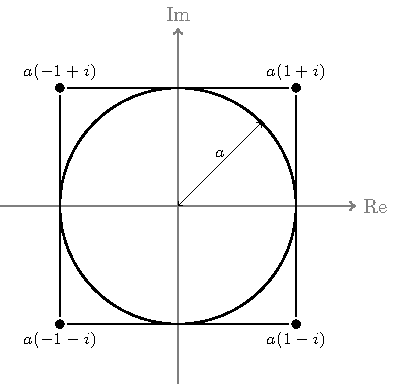
\includegraphics[scale=1]{squareandcircle}
\end{center}
Any point $z$ outside of this circle has modulus $\abs{z} \geq a$; in particular, this is true for any $z \in S_a$.  Hence for all such $z$, $\abs{\dfrac{1}{z}} \leq \dfrac{1}{a}$.

The length of each straight edge of $S_a$ is $2a$, and hence $\ell (S_a) = 8a$.  The Estimation Lemma then gives the required inequality.
\end{answer}

\question Prove each of the following:
\begin{parts}
\part For $z_0$ and $h$ in $\C$ we have $\displaystyle \int_{[z_0,z_0+h]} 1\ dz = h$.
\part For $f:U \to \C$ and $z_0 \in U$, $f(z_0) = \displaystyle \frac{1}{h} \int_{[z_1,z_1+h]} f(z_0)\ dz$.
\part If $\alpha$ is a complex number  and $M$ a fixed real number with $\abs{\alpha} \leq \epsilon M$ for all $\epsilon >0$ then $\alpha=0$.
\end{parts}
\begin{answer}
\begin{parts}
\part Using the parametrisation $\gamma:[0,1] \to \C$, $\gamma(t)=z_0+t(z_0+h-z_0) = z_0+th$, we have
$\gamma'(t)=h$ and $f(\gamma(t))=1$.  Hence
\[
\int_{[z_0,z_0+h]} 1dz = \int_0^1 f(\gamma(t)) \gamma '(t)\ dt = \int_0^1 1 (h) \ dt = h.
\]
Alternatively, using the antiderivative $F(z)=z$ for $f$, we have (by the Fundamental Theorem of Calculus)
\[
\int_{[z_0,z_0+h]} 1dz = F(z_0+h)-F(z_0)=z_0+h-z_0=h.
\]
\part Since $f(z_0)$ is a constant we have
\[
\frac{1}{h} \int_{[z_1,z_1+h]} f(z_0) dz = \frac{1}{h} f(z_0) \int_{[z_1,z_1+h]} 1 dz = \frac{1}{h} f(z_0) h = f(z_0)
\]
by the previous part.
\part Suppose that $\alpha \neq 0$.  Then $\abs{\alpha}>0$ (since for $z \in \C$ we have $\abs{z}=0$ if and only if $z=0$).  Setting $\epsilon = \abs{\alpha}/2M$ we have $\epsilon >0$, which implies that
\[
\abs{\alpha} \leq \epsilon M =  \frac{\abs{\alpha}}{2M} \cdot M = \frac{\abs{\alpha}}{2}.
\]
But this is only possible if $\abs{\alpha} =0$, a contradiction.  Hence $\abs{\alpha}=0$ and so $\alpha=0$.
\end{parts}
\end{answer}


\begin{comment}
\newpage


\question All of the proofs that have been done in lectures are examinable.  As some of these are quite long, you should be prepared to answer questions of the following format, where an outline of the proof is presented in the form of a series of statements.  For each numbered statement, provide a brief comment that explains or justifies it.  

\noindent{\bf Theorem (Cauchy's Theorem for a Triangle) } Let $\mathcal{R}$ be a simply connected region, $f$ a function that is holomorphic on $\mathcal{R}$ and let $T$ be a triangle in $\mathcal{R}$ with boundary $\partial T$.  Then
\[
\int_{\partial T} f =0.
\]
\medskip
{\bf Proof } 
There exists a nested sequence of triangles $\{ T_n \}$ such that
\[
\left( \frac{1}{4} \right)^n \left| \int_{\partial T} f \right| \leq \left| \int_{\partial T_n} f \right| \quad\text{ and }\quad \ell (\partial T_n ) = \left( \frac{1}{2} \right)^n \ell ( \partial T),
\]
and there is a point $z_0 \in \mathcal{R}$ with $z_0 \in T_n$ for all $n$.
\begin{enumerate}
\item[(1)] Given $\varepsilon >0$ there exists $\delta >0$ such that
\[
|z-z_0| < \delta \Longrightarrow \left| f(z)-f(z_0)-(z-z_0)f'(z_0) \right| \leq \varepsilon |z-z_0|
\]
\begin{answer}
Since $f$ is holomorphic on $\mathcal{R}$, $f$ is differentiable at $z_0$ and hence
\[
\lim_{z \to z_0} \frac{f(z)-f(z_0)}{z-z_0}
\]
exists and is equal to $f'(z_0)$.  

By the definition of a limit, given $\varepsilon>0$ there is $\delta >0$ such that
\begin{align*}
0< | z-z_0 | < \delta &\Rightarrow \left| \frac{f(z)-f(z_0)}{z-z_0}-f'(z_0) \right| < \varepsilon \\
& \Rightarrow \left| \frac{f(z)-f(z_0)-(z-z_0)f'(z_0)}{z-z_0} \right| < \varepsilon \\
& \Rightarrow \left| f(z)-f(z_0)-(z-z_0)f'(z_0) \right| < \varepsilon |z-z_0|.
\end{align*}
Finally, if $z=z_0$ then both sides of the final inequality are zero, which shows (1).
\end{answer}
\item[(2)] There exists $n$ such that $\ell ( \partial T_n) < \delta$ and $T_n \subset D(z_0;\delta)$.
\begin{answer}
Since $\ell ( \partial T)$ is fixed, we can choose $n$ large enough so that $\ell ( \partial T)/2^n < \delta$.  By the first (un-numbered) statement, for any such $n$ we have $\ell ( \partial T_n) < \delta$.

Since $z_0$ lies inside $T_n$, the distance from $z_0$ to any point on $\partial T_n$ is less than $\ell ( \partial T_n)$.
\end{answer}

\item[(3)]  For $z \in \partial T_n$
\[
\left| f(z)-f(z_0)-f'(z_0)(z-z_0) \right|< \epsilon \ell ( \partial T_n).
\]
\begin{answer}
By (2), for $z \in \partial T_n$ we have $|z-z_0| < \delta$, hence by (1), for all such $z$ we have
\[
\left| f(z)-f(z_0)-f'(z_0)(z-z_0) \right| \leq \varepsilon | z-z_0 | < \varepsilon \delta < \varepsilon \ell ( \partial T_n )
\]
the final inequality following from (2).
\end{answer}
\item[(4)] \hfil $\displaystyle \int_{\partial T_n} f(z)\ dz = \int_{\partial T_n} \left( f(z)-f(z_0)-f'(z_0)(z-z_0) \right)\ dz$\hfil
\begin{answer}
The (linear) function $z \mapsto f(z_0)+(z-z_0)f'(z_0)$ has an antiderivative on $\mathbb{C}$, and since $\partial T_n$ is a closed path,
\[
\int_{\partial T_n} f(z_0)+(z-z_0)f'(z_0)\ dz =0,
\]
so (4) follows from linearity of path integrals.
\end{answer}
\item[(5)]  \hfil $  \displaystyle \left| \int_{\partial T_n} f \right| \leq \varepsilon\ \left[\ell (\partial T_n ) \right]^2$ \hfil
\begin{answer}
The function $z \mapsto f(z) - f(z_0)-(z-z_0)f'(z_0)$ is bounded above on $\partial T_n$ by $ \varepsilon \ell ( \partial T_n )$ by (3), hence by the Estimation Lemma,
\[
\left| \int_{\partial T_n} f(z) - f(z_0)-(z-z_0)f'(z_0)\ dz \right| \leq \varepsilon \ell ( \partial T_n ) \cdot \ell ( \partial T_n ).
\]
Together with (4), this yields (5).
\end{answer}
\item[(6)] 
\hfil
$
 \displaystyle \left( \frac{1}{4} \right)^n \left| \int_{\partial T} f \right| \leq \left| \int_{\partial T_n} f \right| \leq \varepsilon\ \left[\ell (\partial T_n ) \right]^2 \leq \varepsilon \left(\frac{1}{4} \right)^n \left[ \ell ( \partial T) \right]^2.
$ \hfil
\begin{answer}
The first and last inequalities are given in the first (un-numbered) statement, the second was shown in (4).
\end{answer}
\item[(7)]\hfil $\displaystyle \int_{\partial T} f = 0 .$\hfil
\begin{answer}
By (6) we have
\[
\left| \int_{\partial T} f \right| \leq \varepsilon \left[ \ell ( \partial T ) \right]^2
\]
for all $\varepsilon >0$.  Since $\ell ( \partial T )$ is a constant, (7) follows.
\end{answer}
\end{enumerate}
\end{comment}



\end{questions}
\setcounter{page}{1}
% !TEX root = exercises.tex

\exercisetitle{Exercise Sheet 4}

\begin{questions}
\question Express each of the following complex numbers in Cartesian form $a+ib$:
\[
(a)\ \Log (i), \quad (b)\ \Log (ie)\quad (c)\  \Log (-1-i\sqrt{3}).
\]
\begin{answer}
Using $\Log (z) = \log \abs{z} + i \Arg (z)$,
\begin{align*}
\Log(i) & = \log \abs{i} + i \Arg (i) = \log(1)+i\frac{\pi}{2} = i\frac{\pi}{2}.\\
\Log (ie) &= \log(e)+i\frac{\pi}{2}  = 1 + i \frac{\pi}{2} \\
 \Log (-1-i\sqrt{3}) & =  \log (\sqrt{(-1)^2+(-\sqrt{3})^2}) + i \frac{-2\pi}{3}  = \log(2)-i \frac{2\pi}{3} 
\end{align*}
where $\log:[0,+\infty) \to \R$ denotes the real natural logarithm.
\end{answer}

\question Express each of the following complex numbers in Cartesian form $a+ib$:
\[
 (a)\ (1+i)^i, \quad (b)\ (ie)^{i\pi}, \quad (c)\ (-1-i\sqrt{3})^{1+i}.
\]
\begin{answer}
\begin{align*}
(1+i)^i & = \exp \left( i \Log (1+i) \right) = \exp \left( -\frac{\pi}{4} + i \frac{1}{2} \log(2) \right) \\
& = e^{-\frac{\pi}{4}} \cos ( \frac{1}{2} \log (2) ) + i e^{-\frac{\pi}{4}} \sin ( \frac{1}{2} \log (2) ). \\
(ie)^{i\pi} & = \exp \left( i \pi \Log (ie) \right) \\
& = \exp \left( i\pi - \frac{\pi^2}{2} \right) \\
& = e^{-\frac{\pi^2}{2}} \left( \cos(\pi)+i \sin (\pi) \right) \\
& = -e^{-\frac{\pi^2}{2}} \\
(-1-i \sqrt{3} )^{1+i} & = \exp \left( (1+i) \Log (-1-i \sqrt{3} ) \right) \\
& = \exp \left( (1+i) ( \log (2) - i \frac{2\pi}{3} ) \right) \\
& = \exp \left[ (\log(2)+\frac{2\pi}{3} )+i ( \log(2)- \frac{2\pi}{3}) \right] \\
& = \polar{e^{\log(2) + 2\pi/3}}{\log(2)-2\pi/3} \\
& = 2 \polar{e^{2\pi/3}}{\log(2)-2\pi/3} 
\end{align*}
\end{answer}
\question 
\begin{parts}
\part Use the definition $z^{\alpha} = \exp ( \alpha \Log (z) )$ to show that $z^3 =zzz$.
\part Show that $\Log(i^3) \neq 3 \Log (i)$
\part Define $\sqrt{z} = z^{1/2} ( = \exp ( \frac{1}{2} \Log (z) ) )$ for $z \in \C \backslash \set{0}$.  Where is the mistake in
\[
-1 = i^2 = ii = \sqrt{-1}\sqrt{-1} = \sqrt{-1 \times -1 } = \sqrt{1} =1?
\]
\part Show that for all $\alpha,\beta \in \C$ and $z \in \C \backslash \set{0}$ we have $z^{\alpha}z^{\beta} = z^{\alpha+\beta}$.  Is it true that $\Log(\alpha \beta) = \Log ( \alpha) + \Log ( \beta)$?
\end{parts}
\begin{answer}
\begin{parts}
\part Using the definition of the Principal $3^{rd}$ power function
\begin{align*}
z^3 & = \exp \left( 3 \Log (z) \right) \\
& = \exp \left( \Log(z)+\Log(z)+\Log(z) \right) \\
&= \exp \left(\Log(z) \right)\exp \left(\Log(z) \right)\exp \left(\Log(z) \right) \\
& = zzz.
\end{align*}
\part We have
\[
\Log (i^3) = \Log (-i) = - i\frac{\pi}{2}
\]
while
\[
3 \Log (i) = 3 \left( i \frac{\pi}{2} \right) = i \frac{3\pi}{2}.
\]
\part We do not have
\[
\sqrt{z} \sqrt{w} = \sqrt{zw}
\]
in general.  Indeed
\begin{align*}
\sqrt{-1}\sqrt{-1} & = \exp \left( \frac{1}{2} \Log(-1) \right) \exp \left( \frac{1}{2} \Log (-1) \right) \\
& = \exp ( \Log (-1) ) = -1
\end{align*}
while of course
\[
\sqrt{-1 \times -1 } = \sqrt{1} = \exp \left( \frac{1}{2} \Log (1) \right) = e^0=1.
\]
\part 
\[
z^{\alpha}z^{\beta} = \exp\left( \alpha \Log (z) \right) \exp \left( \beta \Log (z) \right) = \exp\left( (\alpha+\beta) \Log (z) \right) = z^{\alpha+\beta}.
\]
We do not have $\Log(\alpha\beta) = \Log(\alpha)+\Log(\beta)$ in general; for example if $\alpha=-1$ and $\beta=i$, then
\[
\Log(\alpha\beta) = \Log (-i) = -i \frac{\pi}{2}, \text{ while } \Log(\alpha)+\Log(\beta) = i\pi + i \frac{\pi}{2} = i \frac{3\pi}{2}.
\]
\end{parts}
\end{answer}
\question Recall that the Principal Logarithm function $\Log$ is holomorphic on the region $\C_{\pi}$, where \\ $\C_{\pi} = \set{z \in \C:z \neq 0 \text{ and } \Arg (z) \neq \pi }$. Let $F$ be the function defined by
\[
F(z) = \frac{1}{2i} \left( \Log (z+i)-\Log(z-i) \right).
\]
\begin{parts}
\part Describe (or sketch) the region $\mathcal{R}$ on which the function $F$ is holomorphic.
\part Show that $F$ is an antiderivative for the function $f:\mathcal{R} \to \C$ defined by
\[
f(z) = \frac{1}{z^2+1} \quad\text{for all}\quad z \in \mathcal{R}.
\]
\end{parts}
\begin{answer}
In general, for $z_0 = x_0+iy_0 \in \C$, the function
$
z \mapsto \Log (z-z_0)
$
is holomorphic on the region $\set{ z \in \C: z-z_0 \in \C_{\pi} }$.  For $z=x+iy \in \C$, $z-z_0$ is \emph{not} in $\C_{\pi}$ if and only if
\[
z-z_0 = (x-x_0) + i (y-y_0)
\]
lies on the negative real axis.  This occurs when
\begin{itemize}
\item $y-y_0=0$, i.e., when $y=y_0$, and
\item $x-x_0 \leq 0$, i.e. $x \leq x_0$.
\end{itemize}
Hence $z \mapsto \Log (z-z_0)$ is holomorphic on
\[
\C \backslash \set{z = x+iy \in \C: x \leq x_0 \text{ and } y=y_0},
\]
so in particular, $z \mapsto \Log (z+i)$ and $ z \mapsto \Log(z-i)$ are holomorphic on 
\[ \C \backslash \set{x+iy \in \C: x \leq 0 \text{ and } y=-1}\quad\text{ and}\quad \C \backslash \set{x:iy \in \C: x \leq 0 \text{ and } y=1} \]
respectively.

We know that our function $F$ is holomorphic on the region where both $z \mapsto \Log ( z+i)$ and $z \mapsto \Log (z-i)$ are holomorphic; i.e. the intersection of these two sets. This is the set
\[
 \C \backslash \set{ x+iy \in \C: x \leq 0 \text{ and } y= \pm 1 }.
\]

\end{answer}
\question Let $U$ be a starlit region with star centre $z_* \in U$ and  let $g:U \to \C$ be a holomorphic function.
\begin{parts}
\part Prove that if $g(z) \neq 0$ for all $ z \in U$, then the function $\dfrac{g'}{g}$ has an antiderivative on $U$, stating any results used (you may assume that $g$ holomorphic on $U$ implies $g'$ holomorphic on $U$).
\part Prove that if in addition $g(z) \in \C_{\pi}$ for all $z \in U$ then
\[
\int_{[z_*,z]} \frac{g'(\zeta)}{g(\zeta)}\ d\zeta = \Log (g(z)) + \alpha
\]
for some constant $\alpha$.
\end{parts}
\begin{answer}
Since $g$ is holomorphic and nonzero on $U$, $\dfrac{g'}{g}$ is also holomophic on $U$.

By The Existence of Antiderivatives on Starlit Regions, the function $G:U \to \mathbb{C}$ defined by
\[
G(z):= \int_{[z_*,z]} \frac{g'(\zeta)}{g(\zeta)}\ d\zeta
\]
is an antiderivative for $\dfrac{g'}{g}$ on $U$.

Since $\mathrm{Log}$ is holomorphic on $\mathbb{C}_{\pi}$ and $g(z) \in \mathbb{C}_{\pi}$ for all $z \in U$, $z \mapsto \mathrm{Log} (g(z))$ is holomorphic on $U$, with derivative
\[
\frac{d}{dz} \left[ \mathrm{Log} (g(z)) \right] = \frac{g'(z)}{g(z)}.
\]
Together with the first part this shows that
\[
\frac{d}{dz} \left[ \mathrm{Log} (g(z)) - G(z) \right] = 0
\]
on $U$. Since a starlit region is connected, the Fundamental Theorem of Calculus implies that
\[
z \mapsto \mathrm{Log} (g(z)) - G(z) 
\]
is constant.
\end{answer}

\question Evaluate the integral
\[
\int_{\mathcal{C}} \frac{\exp (2z)}{4z+i\pi}\ dz
\]
where $\mathcal{C}$ is (i) the anticlockwise contour whose points lie on the circle $\set{z:\abs{z}=1}$, and (ii) when $\mathcal{C}$ is the anticlockwise contour whose points lie on the circle $\set{z: \abs{z-2i}=2}$. The use of any Theorems made to obtain the value of these integrals should be justified.
\begin{answer}
$(i): \frac{\pi}{2},\quad (ii): 0 $.
\end{answer}
\question Evaluate the integral
\[
\int_{\mathcal{C}} \frac{\cos (z^2)}{3i+2z}\ dz,
\]
where (i) $\mathcal{C}$ is the anticlockwise contour whose points lie on the circle $\set{z:\abs{z}=1}$, and (ii) $\mathcal{C}$ is the anticlockwise contour whose points lie on the circle $\set{z: \abs{z}=5}$.  The use of any Theorems made to obtain the value of these integrals should be justified.
\begin{answer}
(i) The given function is holomorphic on $\C \backslash \set{ z: 3i+2z=0 }$, that is to say, on $\C \backslash \set{ -i \frac{3}{2}}$.  In particular, it is holomorphic on the simply connected region 
\[
\set{ z \in \C: \Im (z) > - \tfrac{5}{4} }
\]
which contains the (closed) contour $\mathcal{C}$.  Thus by Cauchy's Theorem for Starlit regions, 
\[
\int_{\mathcal{C}} \frac{\cos (z^2)}{3i+2z}\ dz=0.
\]

(ii) We have
\[
\frac{\cos(z^2)}{3i+2z} = \frac{g(z)}{z-z_0}
\]
where
\[
z_0 = -i \tfrac{3}{2} \quad \text{ and } \quad g(z) = \tfrac{1}{2} \cos (z^2).
\]
The function $g$ is holomorphic on $\C$ (which is simply connected), and $\mathcal{C}$ is a closed, simple anticlockwise contour that encloses $z_0$, so that by Cauchy's Integral Formula
\[
\int_{\mathcal{C}} \frac{\cos(z^2)}{3i+2z}\ dz = \int_{\mathcal{C}} \frac{g(z)}{z-(-i\frac{3}{2})}\ dz = 2\pi i g(-i \tfrac{3}{2}) = 2\pi i \tfrac{1}{2} \cos (- \tfrac{9}{4}) = i \pi \cos ( \tfrac{9}{4} ).
\]

\end{answer}

\question Evaluate the integral
\[
\int_{-\infty}^{+\infty} \frac{1}{x^2+6x+25}\ dx
\]
in the following way (compare Example 5.8 in the notes):
\begin{parts}
\part Define the complex function $f$ by
$
\displaystyle f(z) = \frac{1}{z^2+6z+25}$  and find $z_0$  and  $z_1$ so that $\displaystyle
f(z) = \frac{1}{(z-z_0)(z-z_1)}$ (where $z_0$ lies in the upper half-plane and $z_1$ in the lower half-plane). 
\begin{answer}
The roots of $z^2+6z+25$ can be found using the quadratic formula;
\begin{align*}
z & = \frac{-6 \pm \sqrt{6^2-4(25)(1)}}{2} \\
& = \frac{-6 \pm \sqrt{-64}}{2} \\
& = \frac{-6+i8}{2} = -3 \pm 4i.
\end{align*}
Hence
\[
f(z) = \frac{1}{(z-(-3+4i))(z-(-3-4i))}.
\]
\end{answer}
\part Choose a suitable function $g$, holomorphic on the simply connected region \\$\mathcal{R} = \set{z \in \C: \Im(z) > \frac{1}{2} \Im (z_1) }$, so that
\[
f(z) = \frac{g(z)}{(z-z_0)}.
\]
\begin{answer}
With $z_0=-3+4i$ and
\[
g(z) = \frac{1}{z-(-3-4i)}
\]
then
\[
f(z) = \frac{g(z)}{z-(-3+4i)}.
\]
Moreover, $g$ is holomorphic on $\C \backslash \set{ -3-4i}$, and in particular, on the simply connected region $\mathcal{R}:= \set{z \in \C: \Im (z) >-2 }$. 
\end{answer}
\part  Justify the use of Cauchy's Integral Formula to find
\[
\int_{\mathcal{C}_R} f = \int_{\mathcal{C}_R} \frac{g(z)}{(z-z_0)}\ dz,
\]
where $\mathcal{C}_R=L_R+S_R$ with $L_R$ the straight line path from $-R$ to $R$ and $S_R$ a suitable semicircular contour from $R$ to $-R$, with $R$  sufficiently large to apply the Theorem.
\begin{answer}
Once $R>5$, the contour simple closed anticlockwise contour $\mathcal{C}_R$ encloses $z_0$.  Moreover $\mathcal{C}_R$ is always contained in the simply connected region $\mathcal{R}$ of the previous part, and $g$ is holomorphic on this region.  Therefore, we may apply Cauchy's Integral formula:
\begin{align*}
\int_{\mathcal{C}_R} f = \int_{\mathcal{C}_R} \frac{g(z)}{z-(-3+4i)}\ dz & = 2\pi i g(-3+4i) \\
& = 2\pi i \cdot \frac{1}{(-3+4i)-(-3-4i)} \\
& = \frac{2\pi i}{8i} = \frac{\pi}{4},
\end{align*}
and this is valid for all $R>5$.
\end{answer}
\part Show that for large $R$ and $z \in S_R$, we have $\abs{z^2+6z+25} \geq R^2-6R-25$.
\begin{answer}
If $z \in S_R$ then $\abs{z}=R$, so that the reverse triangle inequality gives
\begin{align*}
\abs{z^2+6z+25} &\geq \abs{ \abs{z^2} - \abs{6z+25} }\\
& = \abs{\abs{z}^2-\abs{6z+25}} \\
& = \abs{ R^2-\abs{6z+25}}.
\end{align*}
By the triangle inequality,
\[
\abs{6z+25} \leq  6R + 25 \quad \text{ for all } z \in S_R.
\]
Moreover, if $R>10$, we have $25 < 2.5 R$ so that
\[
6R+25 < 6R+2.5 R < 10 R < R^2.
\]
Thus for $R>10$ and $z \in S_R$,
\[
\abs{z^2+6z+25} \geq R^2 - 6R - 25.
\]
\end{answer}
\part Use the Estimation Lemma to show that
\[
\abs{ \int_{S_R} f } \to 0 \text{ as } R \to \infty.
\]
\begin{answer}
By the previous part, for $R>10$ and $z \in S_R$ we have
\[
\abs{
\frac{1}{z^2+6z+25}
}
 \leq \frac{1}{R^2-6R-25}.
\]
Since the length of $S_R$ is $\pi R$, for all $R>10$ we have
\[
\abs{\int_{S_R} f} \leq \underbrace{\frac{1}{R^2-6R-25}}_{M} \cdot \underbrace{\pi R}_L = \frac{\pi}{R-6-\frac{25}{R}}
\]
by the Estimation Lemma.  Hence
\[
\abs{ \int_{S_R}} f \to 0 \quad \text{ as }\quad R \to \infty.
\]
\end{answer}
\part Deduce the value of
\[
\int_{-\infty}^{+\infty} \frac{1}{x^2+6x+25}\ dx.
\]
\begin{answer}
We have
\begin{align*}
\frac{\pi}{4} & = \int_{\mathcal{C}_R} f && \text{ for } R>5 \\
& = \lim_{R \to \infty} \left( \int_{C_R} f \right) && \\
&=  \lim_{R \to \infty} \left( \int_{L_R} f \right) + \lim_{R \to \infty} \left( \int_{S_R} f \right) && \\
& = \lim_{R \to \infty} \left( \int_{-R}^{R} \frac{1}{t^2+6t+25}\ dt \right) + 0 && \text{ by part (d) } \\
& = \int_{-\infty}^{\infty} \frac{1}{x^2+6x+25}\ dx. &&
\end{align*}

\end{answer}
\end{parts}

\question (Liouville's Theorem) Let $f:\C \to \C$ be holomorphic everywhere, and suppose that $f$ is bounded, i.e. there exists $M>0$ with $\abs{f(z)} \leq M$ for all $z \in \C$.  Show that $f$ is constant on $\C$, in the following way:
\begin{parts}
\part Let $z_1,z_2 \in \C$, and let $R>0$ be sufficiently large so that $z_1$ and $z_2$ are enclosed by the countour $\mathcal{C}_R$ consisting of the anticlockwise circle with centre $0$ and radius $R$. Use Cauchy's Integral Formula to write $f(z_1)-f(z_2)$ as a single integral along $\mathcal{C}_R$.
\begin{answer}
As $f$ is holomorphic on $\C$ and $\mathcal{C}_R$ is a simple, closed anticlockwise contour containing both $z_1$ and $z_2$, we can apply Cauchy's Integral formula (twice) to get
\[
\int_{\mathcal{C}_R} \frac{f(z)}{z-z_1}\ dz = 2 \pi i f(z_1) \quad \text{ and }\quad \int_{\mathcal{C}_R} \frac{f(z)}{z-z_2}\ dz = 2 \pi i f(z_2).
\]
Hence (since we may combine integrals along the same path)
\begin{align*}
f(z_1)-f(z_2) & = \frac{1}{2\pi i} \int_{\mathcal{C}_R} \frac{f(z)}{z-z_1}\ dz - \frac{1}{2\pi i} \int_{\mathcal{C}_R} \frac{f(z)}{z-z_2}\ dz \\
& = \frac{1}{2\pi i} \int_{\mathcal{C}_R} \left( \frac{f(z)}{z-z_1} - \frac{f(z)}{z-z_2} \right)\ dz \\
& = \frac{1}{2\pi i} \int_{\mathcal{C}_R} \frac{f(z)(z-z_2)-f(z)(z-z_1)}{(z-z_1)(z-z_2)}\ dz \\
& = \frac{1}{2\pi i} \int_{\mathcal{C}_R} \frac{f(z)(z_1-z_2)}{(z-z_1)(z-z_2)}\ dz.
\end{align*}
\end{answer}
\part Use the Estimation Lemma (and the backwards triangle inequality) to show that
\[
\abs{f(z_1)-f(z_2)} \leq M \frac{\abs{z_1-z_2}}{(R-\abs{z_1})(R-\abs{z_2})}\cdot 2\pi R
\]
for all (sufficiently large) $R$.
\begin{answer}
If $R> \max ( \abs{z_1}, \abs{z_2} )$ and $z \in \mathcal{C}_R$, then by the backwards triangle inequality
\[
\abs{z-z_1} \geq \abs{ \abs{z} - \abs{z_1}} = R - \abs{z_1}
\]
and similarly $\abs{z-z_2} \geq R - \abs{z_2}$.  Since $\abs{f(z)} \leq M$ we have
\begin{align*}
\abs{ \frac{f(z)(z_1-z_2)}{(z-z_1)(z-z_2)} }  &= \frac{\abs{f(z)} \cdot \abs{z_1-z_2}}{\abs{z-z_1} \cdot \abs{z-z_2}} \\
& \leq \frac{M \abs{z_1-z_2}}{(R-\abs{z_1})(R-\abs{z_2})}.
\end{align*}
The path $\mathcal{C}_R$ has length $2 \pi R$, thus by the Estimation Lemma
\[
\abs{ \int_{\mathcal{C}_R} \frac{f(z)(z_1-z_2)}{(z-z_1)(z-z_2)}\ dz } \leq M \frac{\abs{z_1-z_2}}{(R-\abs{z_1})(R-\abs{z_2})}\cdot 2\pi R
\]
\end{answer}
\part Deduce that $f(z_1)=f(z_2)$.
\begin{answer}
By parts (b) and (c) we have
\begin{align*}
\abs{f(z_1)-f(z_2)} &= \abs{ \frac{1}{2\pi i} \int_{\mathcal{C}_R} \frac{f(z)(z_1-z_2)}{(z-z_1)(z-z_2)}\ dz } \\
& \leq \abs{ \frac{1}{2\pi i} }  M \frac{\abs{z_1-z_2}}{(R-\abs{z_1})(R-\abs{z_2})}\cdot 2\pi R \\
& = \frac{MR \abs{z_1-z_2}}{(R-\abs{z_1})(R-\abs{z_2})} \\
& = \frac{M \abs{z_1-z_2}}{(1-\abs{z_1}/R)(R-\abs{z_2})}
\end{align*}
for all $R>\max(\abs{z_1},\abs{z_2})$.  Since $M$ and $\abs{z_1-z_2}$ are constants, it follows that
\[
\frac{M \abs{z_1-z_2}}{(1-\abs{z_1}/R)(R-\abs{z_2})} \to 0 \quad\text{as}\quad R \to \infty.
\]
Hence $\abs{f(z_1)-f(z_2)}=0$, or in other words $f(z_1)=f(z_2)$.
\end{answer}
\end{parts}
\end{questions}
\setcounter{page}{1}
% !TEX root = exercises.tex

\exercisetitle{Exercise Sheet 5}

\begin{questions}
\question Locate the poles of each of the following functions, and calculate the residues at these poles:
\begin{parts}
\part $f(z) = \dfrac{1}{z(i-z)^3}$
\part $f(z) = \dfrac{z^2}{(z^2+1)^2}$
\part $f(z) = \dfrac{\Log(z)}{(4z-i)^2}$
\part $f(z)=\dfrac{1}{\exp(z)-1}$.
\end{parts}
\begin{answer}
\begin{parts}
\part This time $f$ has a pole of order $1$ at $0$ and a pole of order $3$ at $i$.  With $g_1(z) = \frac{1}{(i-z)^3}$ and $h_1(z)=z$, the $g/h$ rule gives
\[
\Res (f;0) = \frac{g(0)}{h'(0)} = \frac{1}{(1) \cdot (i)^3}  = i.
\]
For the pole of order $3$ at $i$ we first rewrite
\[
f(z) = \frac{1}{z(-(z-i))^3} = - \frac{1}{z(z-i)^3}.
\]
Now, letting $g_2(z) = -z^{-1}$ we can use the formula
\[
\Res (f;i) = \frac{g_2''(i)}{2!}.
\]
We have $g_2'(z) = z^{-2}$ and $g_2''(z) = -2z^{-3}$, so that $g_2''(i)=-2/(i)^3 = -2i$ and hence
\[
\Res (f;i) = \frac{-2i}{2} = -i.
\]
\part Writing
\[
f(z) = \frac{z^2}{(z+i)^2(z-i)^2}
\]
we see that $f$ has poles of order $2$ at $z=\pm i$.  If $g_1 (z)=  \dfrac{z^2}{(z+i)^2}$ then
\[
g_1'(z) = \frac{(z+i)^2(2z)-2(z+i)z^2}{(z+i)^4},\quad g_1'(i) = \frac{(2i)^3-2(2i)i^2}{(2i)^4} = - \frac{i}{4}
\]
hence
\[
\Res (f; i) = \frac{g_1'(i)}{1!} = - \frac{i}{4}.
\]
Similarly, with $g_2(z) = \frac{z^2}{(z-i)^2}$,
\[
g_2'(z) = \frac{(z-i)^2(2z)-2(z-i)z^2}{(z-i)^4},\quad g_2'(-i) = \frac{(-2i)^2(2i)-2(-2i)(-2i)^2}{(-2i)^4} = \frac{i}{4}.
\]
Hence
\[
\Res (f;-i) = \frac{g_2'(i)}{1!} = \frac{i/4}{1} = \frac{i}{4}.
\]
\part Pole of order $2$ at $z=i/4$.  Write $f(z) = \dfrac{\Log(z)}{16 (z-\frac{i}{4})^2}$, then
\[
\Res(f;i/4) = \frac{1}{16} \cdot \frac{1}{(i/4)} = - \frac{i}{4}.
\]
\part Use the $g/h$ rule with $g(z)=1$ and $h(z)=\exp(z)-1$.  Then $h(z)=0$ whenever $\exp(z)=1$, i.e. at the points $z_k = 2\pi i k$ where $k \in \mathbb{Z}$, so $f$ has isolated singularities at these points.  Since $h'(z) = \exp(z),\ h'(z_k)=1$ for all $k$, and so each $z_k$ is a pole of order $1$ for the function $f$.  By the $g/h$ rule,
\[
\Res (f;z_k) = \frac{g(z_k)}{h'(z_k)} = 1.
\]
\end{parts}


\end{answer}
\question Evaluate
\[
\int_{\mathcal{C}} \frac{1}{z(z-1)(z+2)}\ dz,
\]
where $\mathcal{C}$ is the anticlockwise circle with centre $0$ and radius $3/2$.
\begin{answer}
The function $f$ defined by
\[
f(z) = \frac{1}{z(z-1)(z+2)}
\]
has isolated singularities at $0,1$ and $2$, and the first two of these are enclosed by $\mathcal{C}$.  The residues are
\begin{align*}
\Res (f;0) &= \frac{1}{(0-1)(0+2)}  = - \frac{1}{2} \\
 \Res (f;1) & = \frac{1}{1(1+2)}  = \frac{1}{3}.
\end{align*}
Hence by the Residue Theorem
\[
\int_{\mathcal{C}} \frac{1}{z(z-1)(z+2)}\ dz = 2\pi i \left( - \frac{1}{2} + \frac{1}{3} \right) = - \frac{i\pi}{3}.
\]
\end{answer}
\question Evaluate
\[
\int_{\mathcal{C}} \frac{1}{(z^2+1)^3}\ dz
\]
where $\mathcal{C}$ is the anticlockwise square with vertices $1,\ 1+2i, -1+2i$ and $-1$.
\begin{answer}
Using the factorisation $(z^2+1)^3=(z+i)^3(z-i)^3$, we see that this function, call it $f$, has poles of order $2$ at $z=\pm i$.  Of these, only the pole at $z=i$ is enclosed by $\mathcal{C}$, so that 
\[
\int_{\mathcal{C}} \frac{1}{(z^2+1)^3}\ dz = 2\pi i \Res (f;i).
\]
If we let $g(z) = \dfrac{1}{(z+i)^3}$ then
\[
f(z) = \frac{g(z)}{(z-i)^3},
\]
$g'(z) = -3 (z+i)^{-4}$ and $g''(z) = 12(z+i)^{-5}$.  Hence
\[
\Res (f;i) = \frac{g''(i)}{2!} = \frac{12}{2(2i)^5} = \frac{3}{16i}
\]
which gives
\[
\int_{\mathcal{C}} f = 2\pi i \left( \frac{3}{16i} \right) = \frac{3\pi}{8}.
\]
\end{answer}
\question Use contour integration to evaluate each of the following real integrals:
\begin{parts}
\part \hfil$\displaystyle
\int_0^{2\pi} \frac{1}{5+4 \sin \theta}\ d\theta 
$\hfil
\part \hfil$\displaystyle \int_0^{\infty} \frac{1}{x^4+1}\ dx$\hfil
\end{parts}
\begin{answer}
\begin{parts}
\part We use the fact that for a rational function $R$ of two (real) variables,
\[
\int_0^{2\pi} R( \cos(t), \sin (t) ) dt = \int_{\mathcal{C}} f
\]
where $\mathcal{C}$ is the anticlockwise unit circle and $f$ is the complex function defined by
\[
f(z) = R \left( [z+z^{-1}]/2 , [z-z^{-1}]/(2i) \right) \cdot \frac{1}{iz}.
\]
In this case, we have
\begin{align*}
f(z) & = \frac{1}{5+4[z-z^{-1}]/2i} \cdot \frac{1}{iz} \\
& = \frac{1}{2z^2+5iz-2} \\
& = \frac{1}{(2z+i)(z+2i)}.
\end{align*}
Then with $\mathcal{C}$ the anticlockwise unit circle, the only singularity of $f$ enclosed by $\mathcal{C}$ is at $z=-i/2$, and so
\begin{align*}
\int_0^{2\pi} \frac{1}{5+4 \sin \theta}\ d\theta &= \int_{\mathcal{C}} \frac{1}{(2z+i)(z+2i)}\ dz \\
& = 2\pi i \Res (f;-i/2) \\
& = 2\pi i \cdot \frac{1}{2(-i/2+2i)} = \frac{2\pi}{3}.
\end{align*}
\part 
We shall consider the complex function
\[
f(z) = \frac{1}{z^4+1}
\]
which is holomorphic everywhere in $\C$ except where $z^4=-1$; that is to say, $f$ is holomorphic on $\C \backslash \set{ e^{i\pi/4},\ e^{i3\pi/4},\ e^{i 5\pi/4},\ e^{i 7\pi/4} }$.  Let $\mathcal{C}_R = L_R+S_R$ where $R>1$, $L_R$ is the straight line path $[-R,R]$ and $S_R$ is the upper-semicircle with centre $0$ and radius $R$ from $R$ to $-R$ via $iR$; then the poles of $f$ enclosed by $\mathcal{C}_R$ are at $e^{i\pi/4}$ and $e^{i3\pi/4}$.

With $g(z)=1$ and $h(z)=z^4+1$, we have $h'(z)=4z^3$ so that by the $g/h$ rule,
\begin{align*}
\Res(f;e^{i\pi/4}) &= \frac{1}{4(e^{i\pi/4})^3} = \frac{1}{4e^{3\pi/4}} = \frac{1}{4(-a+ia)} \\
\Res(f;e^{i3\pi/4}) &= \frac{1}{4(e^{i3\pi/4})^3} = \frac{1}{4e^{9\pi/4}} = \frac{1}{4(a+ia)} \\
\end{align*}
where $a=1/\sqrt{2}$. So (for $R>1$) we have
\begin{align*}
\int_{\mathcal{C}_R} f &= 2\pi i \left( \text{ sum of residues at poles of $f$ inside $\mathcal{C}_R$} \right) \\
& = 2\pi i \left( \frac{1}{4(-a+ia)}+\frac{1}{4(a+ia)}) \right)
& = \frac{\pi}{\sqrt{2}}
\end{align*}
by the Residue Theorem.

We now show that 
\[
\lim_{R \to \infty} \int_{S_R} f =0
\]
using the Estimation Lemma.  Indeed, for $z \in S_R$, $\abs{z}=R$ and so by the reverse triangle inequality
\[
\abs{z^4+1} \geq \abs{ \abs{z^4} - \abs{1} } = \abs{ \abs{z}^4-1 } = R^4-1.
\]
Hence for all such $z$,
\[
\abs{ f(z) } = \abs{\frac{1}{z^4+1}} = \frac{1}{\abs{z^4+1}} \leq \frac{1}{R^4-1}.
\]
The Estimation Lemma then gives
\[
\abs{ \int_{S_R} f } \leq \frac{1}{R^4-1} \cdot \pi R = \frac{\pi R}{R^4-1}
\]
so that
\[
\int_{S_R} f \to 0 \quad\text{ as }\quad R \to \infty.
\]

Using the parametrisation $\gamma_L:[-R,R] \to \C$, $\gamma(t)=t$ of $L_R$, we have
\[
\int_{L_R} f = \int_{-R}^R \frac{1}{(t^4+1}\ dt.
\]
Hence
\begin{align*}
\frac{\pi}{\sqrt{2}} & = \int_{\mathcal{C}_R} f \\
& = \lim_{R \to \infty} \int_{\mathcal{C}_R} f \\
& = \lim_{R \to \infty} \int_{-R}^R \frac{1}{t^4+1}\ dt + \lim_{R \to \infty} \int_{S_R} f \\
& = \int_{-\infty}^{\infty} \frac{1}{t^4+1}\ dt.
\end{align*}
Since the integrand is even, it follows that
\[
\int_{0}^{\infty} \frac{1}{t^4+1}\ dt = \frac{1}{2} \int_{-\infty}^{\infty} \frac{1}{t^4+1}\ dt = \frac{\pi}{2\sqrt{2}}.
\]

\end{parts}
\end{answer}
\question Use contour integration to evaluate the following real integrals:
\begin{parts}
\part \[
\int_0^{2\pi} \frac{1}{16 \cos^2 (t)+25 \sin^2 (t)}\ dt.
\]
\begin{answer}
As before, we use the fact that for a rational function $R$ of two (real) variables,
\[
\int_0^{2\pi} R( \cos(t), \sin (t) ) dt = \int_{\mathcal{C}} f
\]
where $\mathcal{C}$ is the anticlockwise unit circle and $f$ is the complex function defined by
\[
f(z) = R \left( [z+z^{-1}]/2 , [z-z^{-1}]/(2i) \right) \cdot \frac{1}{iz}.
\]
Here $f$ is given by
\begin{align*}
f(z) = \frac{4iz}{9z^4-82z^2+9},
\end{align*}
and so
\[
\int_{\mathcal{C}} \frac{4iz}{9z^4-82z^2+9}\ dz
\]
where $\mathcal{C}$ is the anticlockwise unit circle.  Factorising the denominator gives
\[
9z^4-82z^2+9 = (9z^2-1)(z^2-9) = (3z-i)(3z+i)(z-3i)(z+3i),
\]
and so the poles of $f$ enclosed by $\mathcal{C}$ are at $z= \pm i/3$.  Hence by the Residue Theorem
\[
\int_{\mathcal{C}} f = 2\pi i \left[ \Res (f;i/3)+ \Res (f;-i/3) \right] = \frac{\pi}{10}
\]
and so
\[
\int_0^{2\pi} \frac{1}{16 \cos^2 (t)+25 \sin^2 (t)}\ dt = \frac{\pi}{10}.
\]


\end{answer}
\part
\[
\int_{-\infty}^{\infty} \frac{1}{(x^2+1)(x^2+9)}\ dx.
\]
\begin{answer}
With $\displaystyle f(z)=\frac{1}{(z^2+1)(z^2+9)} = \frac{1}{z^4+10z+9}$, $R>3$ and $\mathcal{C}_R=L_R+S_R$ as before, the Residue Theorem gives
\[
\int_{\mathcal{C}_R} f = 2\pi i \left( \Res(f;i)+\Res(f;3i) \right) = \frac{\pi}{12}.
\]
The reverse triangle inequality gives
\[
\abs{\frac{1}{(z^2+1)(z^2+9)}} \leq \frac{1}{(R^2-1)(R^2-9)}
\]
for all $z \in S_R$ so that by the Estimation Lemma
\[
\abs{ \int_{S_R} f } \leq \frac{\pi R}{(R^2-1)(R^2-9)} \to 0 \quad\text{as}\quad R \to \infty.
\]
A similar argument to the one used before yields
\[
\int_{-\infty}^{+\infty} \frac{1}{(x^2+1)(x^2+9)}\ dx = \frac{\pi}{12}.
\]
\end{answer}
\part \[
\int_0^{\infty} \frac{\cos(5x)}{x^2+4}
\]
(Hint: first use the usual method to evaluate
$
\displaystyle \int_{-\infty}^{+\infty} \frac{e^{i5x}}{x^2+4}\ dx.
$)
\begin{answer}
Following the hint, we let $f(z) = \dfrac{\exp(5iz)}{z^2+4}$, and consider the contour $\mathcal{C}_R=L_R+S_R$ as before, where $R>2$.  Using the Residue Theorem we get
\[
\int_{\mathcal{C}_R} f = 2 \pi i  \Res (f;2i) = \frac{\pi}{2}e^{-10}.
\]
For $z=x+iy \in S_R$ we have
\begin{align*}
\abs{\exp(5iz)} &= \abs{\exp (5i(x+iy))} \\
& = \abs{\exp(-5y+5ix)} \\
& = \abs{\polar{e^{-5y}}{5x}} \\
& = \abs{e^{-5y}} \abs{\cos(5x)+i\sin(5x)} = e^{-5y}.
\end{align*}
Since $S_R$ lies above the real axis, $x+iy \in S_R$ implies $y\geq 0$, so that $-5y \leq 0$ and so $e^{-5y} \leq e^0=1$.  Thus $\abs{\exp(5iz)} \leq 1$ for all $z \in S_R$.

By the reverse triangle inequality $\abs{z^2+4} \geq R^2-4$ for all $z \in S_R$, thus for all such $z$,
\[
\abs{f(z)} \leq \frac{1}{R^2-4}.
\]
Together with the Estimation Lemma we see that
\[
\abs{\int_{S_R} f } \leq \pi R \cdot \frac{1}{R^2-4} \to 0 \quad\text{as}\quad R \to \infty.
\]
Arguing as before, we get
\[
\int_{-\infty}^{+\infty} \frac{e^{5ix}}{x^2+4}\ dx = \frac{\pi}{2}e^{-10}.
\]
Now, for all $x \in \R$, $e^{5ix} = \cos(5x)+i\sin(5x)$, so that
\[
\int_{-\infty}^{+\infty}  \frac{e^{5ix}}{x^2+4}\ dx = \int_{-\infty}^{+\infty} \frac{\cos(5x)}{x^2+4}\ dx \ + i \int_{-\infty}^{+\infty} \frac{\sin(5x)}{x^2+4}\ dx
\]
or in other words
\[
\int_{-\infty}^{+\infty} \frac{\cos(5x)}{x^2+4}\ dx = \Re \left( \int_{-\infty}^{+\infty}  \frac{e^{5ix}}{x^2+4}\ dx \right) = \frac{\pi}{2} e^{-10}.
\]
Finally, since the integrand is even,
\[
\int_0^{\infty} \frac{\cos(5x)}{x^2+4}\ dx = \frac{1}{2} \left( \int_{-\infty}^{+\infty} \frac{\cos(5x)}{x^2+4}\ dx \right) = \frac{\pi}{4} e^{-10}.
\]
\end{answer}
\end{parts}
\question
\begin{parts}
\part Let $N$ be a natural number and let $\alpha_j$ be constants for $-N \leq j \leq N$.  If $f(z) = \displaystyle \sum_{j=-N}^N \alpha_j z^j$, write down the value of $\Res(f;0)$.
\part Write $\displaystyle \int_0^{2\pi} \left[ \cos(t) \right]^{8}\ dt$ as a contour integral, and use part (a) to evaluate it.
\end{parts}
\begin{answer}
Let $\mathcal{C}$ be the anticlockwise circle with centre $0$ and radius $1$, so that
\[
\Res (f;0) = \frac{1}{2\pi i} \int_{\mathcal{C}} f
\]
We know that for $n \neq -1$, the function $z \mapsto z^n$ has an antiderivative on $\C \backslash \set{0}$, hence  $\displaystyle \int_{\mathcal{C}} z^n\ dz =0$ for $n \neq -1$.  It follows that
\begin{align*}
\Res (f;0)  = \frac{1}{2\pi i}\int_{\mathcal{C}} f & = \frac{1}{2\pi i} \int_{\mathcal{C}} \sum_{j=-N}^N \alpha_j z^j\ dz \\
& = \frac{1}{2\pi i} \sum_{j=-N}^N \alpha_j \int_{\mathcal{C}} z^j\ dz \\
& = \frac{1}{2\pi i} \alpha_{-1} \int_{\mathcal{C}}  z^{-1}\ dz \\
& =  \frac{1}{2\pi i} \cdot \alpha_{-1} \cdot 2\pi i = \alpha_{-1}.
\end{align*}
For (b), following previous examples we know that
\[
\int_0^{2\pi} \left( \cos(t) \right)^{8}\ dt = \int_{\mathcal{C}} \left( \frac{z+z^{-1}}{2} \right)^8 \cdot \frac{1}{iz}\ dz
\]
The binomial formula allows us to expand
\[
(z+z^{-1})^8 = \sum_{k=0}^8\binom{8}{k} z^k(z^{-1})^{8-k} = \sum_{k=0}^8\binom{8}{k} z^{2k-8},
\]
hence
\[
\frac{1}{iz} \left( \frac{z+z^{-1}}{2} \right)^8 = \frac{1}{i2^8} \sum_{k=0}^8\binom{8}{k} z^{2k-9}.
\]
The only isolated singularity of this function is at $z=0$, and by part (a), $\Res(f;0)$ is simply the coefficient of $z^{-1}$, i.e. $\frac{1}{i2^8}\binom{8}{4} =\frac{35}{128i}$.  By the Residue Theorem,
\[
\int_{\mathcal{C}} f = 2\pi i \frac{35}{128i} = \frac{35\pi}{64}.
\] 
\end{answer}

\end{questions}
\setcounter{page}{1}
\end{document}" > main.tex
% $pdflatex main.tex
% 

% document class
\documentclass[oneside, 11pt]{article}

\usepackage{amsthm}
\usepackage[cm]{fullpage}

\usepackage[margin=30mm]{geometry}

\usepackage{camnotes}
\answercolour{blue}

% module info
%\modulecode{MA2003}
%\moduletitle{Complex Analysis I}
%\academicyear{2017-18}

%\renewcommand{\thetheorem}{\arabic{chapter}.\arabic{theorem}}
% load packages
\usepackage{amsmath}
\usepackage{comment}
\usepackage{verbatim}
\usepackage{mathtools}
\usepackage{amsfonts}
\usepackage{amssymb}
\usepackage{wrapfig}
\usepackage{setspace}

\usepackage{framed}
\usepackage{enumitem}
\usepackage{array}
\usepackage{xcolor}
\usepackage{float}
\usepackage[mode=buildnew]{standalone}% requires -shell-escape
\usepackage{sidecap}
\usepackage{version}
\usepackage{todonotes}
\sidecaptionvpos{figure}{r}
\renewcommand\sidecaptionsep{2cm}

\setstretchfactor{1.5} 
\setimagestretchfactor{1}
\setboxrule{0.5pt}

% document info
\title{Exercise Sheets}
\author{D McConnell}
\date{Summer 2017}

\graphicspath{{./images/}}

% new commands
\newcommand{\contint}{\int_{\mathcal{C}}}
\newcommand{\conj}[1]{\overline{#1}}
\newcommand{\conjugate}[1]{\overline{#1}}
\renewcommand{\Re}{\textsf{Re}}
\renewcommand{\Im}{\textsf{Im}}
\newcommand{\abs}[1]{\left| #1 \right|}
\newcommand{\set}[1]{\left\{#1\right\}}
\newcommand{\brac}[1]{\left( #1 \right) }
\newcommand{\pd}[2]{\dfrac{\partial #1}{\partial #2}}
\newcommand{\rlim}[2]{\lim_{\substack{#1, \\ #2}}}
\newcommand{\reverse}[1]{\widetilde{#1}}
\newcommand{\id}{\textsf{id}}
\newcommand{\Res}{\mathrm{Res}}
\newcommand{\Arg}{\mathrm{Arg}}
\newcommand{\polar}[2]{#1 \left( \cos \left( #2 \right) + i \sin \left( #2 \right) \right)}
\newcommand{\expform}[2]{ #1 \exp \left( #2 \right)}
\newcommand{\R}{\mathbb{R}}
\newcommand{\C}{\mathbb{C}}
\newcommand{\cont}{\mathcal{C}}
\newcommand{\less}[1]{\backslash \set{#1}}

\DeclareMathOperator{\Log}{Log}

\newcommand{\leftimage}[2]{
\begin{tabular}{c@{\hskip 1cm} m{0.5\textwidth} }
\begin{minipage}{0.5\textwidth}
\begin{center}
\begingroup
#1
\endgroup
\end{center}
\end{minipage}
&
\blankson\begingroup
#2
\endgroup\blanksoff
\end{tabular}
}

\newcommand{\exercisetitle}[1]{\begin{center}{\large\bf MA2003 Complex Analysis \\#1}\end{center}\bigskip}

%\includeonly{ex1_source}

\begin{document}
% !TEX root = exercises.tex

\exercisetitle{Exercise Sheet 0}

\begin{questions}
\question Write the following complex numbers in polar form $z=r \left( \cos ( \theta)+ i \sin (\theta) \right)$ (or equivalently, $z=r \exp \left(i \theta \right)$):
\begin{parts}
\part $1+i$
\part $-1+i$
\part $1+i \sqrt{3}$
\part $\dfrac{(1+i)^7}{(1+i\sqrt{3})^2}$
\end{parts}

\begin{answer}
\begin{enumerate}
\item[(a)] $1+i=\sqrt{2} \left( \cos ( \frac{\pi}{4} ) + i \sin ( \frac{\pi}{4} ) \right)$
\item[(b)] $-1+i=\sqrt{2} \left( \cos ( \frac{3\pi}{4} ) + i \sin ( \frac{3\pi}{4} ) \right)$
\item[(c)] $1+i\sqrt{3}=2 \left( \cos ( \frac{\pi}{3} ) + i \sin ( \frac{\pi}{3} ) \right)$
\item[(d)] While we could expand the numerator and denominator and then simplify, it is much easier to use De Moivre's Theorem:
\[
r \left( \cos ( \theta) + i \sin (\theta ) \right)^n = r^n \left( \cos ( n\theta) + i \sin ( n \theta ) \right) \quad (n \in \mathbb{Z}).
\]
\begin{align*}
(1+i)^7 & = \polar{2^{7/2}}{7 \pi / 4},\\ 
(1+ i \sqrt{3})^{-2} & = \polar{2^{-2}}{-2\pi/3}.
\end{align*}
Then we get
\begin{align*}
\frac{(1+i)^7}{(1+i\sqrt{3})^2} & = (1+i)^7(1+i \sqrt{3})^{-2} \\
& = \polar{2^{3/2}}{13\pi/12}. 
\end{align*}
This is fine, however, if we wish to use the principal value of the argument, we must subtract an appropriate integer multiple of $2\pi$ from $13\pi/12$ (to ensure that the argument lies in $(-\pi,\pi]$).  This is given by  $13\pi /12-2\pi = -11\pi/12$, thus
\[
\frac{(1+i)^7}{(1+i\sqrt{3})^2} = \polar{2^{3/2}}{-11\pi /12}.
\]
An equally valid way of answering this is using the exponential polar form:
\[
(1+i)^7 = \expform{2^{7/2}}{7 \pi / 4}\qquad(1+ i \sqrt{3})^{-2} = \expform{2^{-2}}{-2\pi/3}.
\]
The properties $\exp(z_1)\exp(z_2)=\exp(z_1+z_2)$ and $\exp(z+2\pi i)=\exp(z)$  give:
\[
\frac{(1+i)^7}{(1+i\sqrt{3})^2} = \expform{2^{7/2}}{7 \pi/4} \expform{2^{-2}}{-2\pi/3}  =  \expform{2^{3/2}}{-11\pi/12}.
\]
\end{enumerate}
\end{answer}

\question 
\begin{parts}
\part For $z=a+ib$, express $z^{-1}$ (i.e, $\dfrac{1}{z}$) in Cartesian form
\part Write down the modulus and Principal Argument of $z^{-1}$ in terms of $\abs{z}$ and $\Arg (z)$.
\end{parts}

\begin{answer}
\begin{enumerate}
\item[(a)] We use the fact that $\displaystyle \frac{1}{z} = \frac{1}{z} \cdot \frac{\conj{z}}{\conj{z}} = \frac{\conj{z}}{\abs{z}^2}$ to invert any nonzero complex number:
\[
\frac{1}{a+ib} = \frac{1}{a+ib} \cdot \frac{a-ib}{a-ib} = \frac{a-ib}{a^2+b^2} = \frac{a}{a^2+b^2} - i\frac{b}{a^2+b^2}.
\]
\item[(b)] Writing $z=\polar{r}{\theta}$, De Moivre's Theorem gives
\[
z^{-1} = \left(\polar{r}{\theta}\right)^{-1} = \polar{\frac{1}{r}}{-\theta}.
\]
Hence $\abs{z^{-1}} = 1/\abs{z}$ and $\Arg (z^{-1})=-\Arg (z)$.
\end{enumerate}
\end{answer}

\question Express the following complex numbers in Cartesian form (that is to say, as $a+ib$ for $a,b \in \R$)
\[
\frac{i-1}{1-i}\qquad \frac{1}{1+i}\qquad \frac{3+4i}{1-2i}.
\]
\begin{answer}
In each case, we make the denominator of the quotient $\frac{z_1}{z_2}$ real by multiplying by $\conj{z_2}/ \conj{z_2}$, which gives
\[
\frac{z_1}{z_2} = \frac{z_1\conj{z_2}}{\abs{z_2}^2}.
\]
Thus for example
\begin{align*}
\frac{i-1}{1-i} & = \frac{i-1}{1-i} \cdot \frac{1+i}{1+i} \\
& = \frac{1}{2} \left[ i(1+i)-1(1+i) \right] \\
& = \frac{1}{2} \left[-2 \right] \\
& = -1\ (+i0).
\end{align*}
Similarly
\begin{align*}
\frac{1}{1+i} &=  \frac{1}{2} - \frac{i}{2} \\
\frac{3+4i}{1-2i} &= -1+2i.
\end{align*}
\end{answer}

\question Find the principal argument of the four points $\pm 1\pm i\sqrt{3}$.
\begin{answer}
\begin{align*}
\Arg (1+i\sqrt{3}) &= \frac{\pi}{3} \\
\Arg (-1+i \sqrt{3} ) &= \frac{2\pi}{3} \\
\Arg (-1-i\sqrt{3} ) &= - \frac{2\pi}{3} \\
\Arg (1-i\sqrt{3} ) &= - \frac{\pi}{3}. 
\end{align*}
\end{answer}




\question Calculate
\[
\Arg \left. \left( \frac{1}{2} + \frac{1}{z^2} \right) \right|_{z=1+i}.
\]
(The notation
$
\left. f(z) \right|_{z=w}
$
means $f(z)$ evaluated at $z=w$, or in other words, $f(w)$.)
\begin{answer}
We have
\[
\frac{1}{2} + \frac{1}{(1+i)^2} = \frac{1}{2}-\frac{i}{2},
\]
with principal argument $-\frac{\pi}{4}$.
\end{answer}
\question Show that
\[
2 \left( \frac{z}{z+i} \right) \left. \frac{(z+i-z)}{(z+i)^2} \right|_{z=i} = \frac{-i}{4}.
\]
\begin{answer}
\begin{align*}
2 \left( \frac{z}{z+i} \right) \left. \frac{(z+i-z)}{(z+i)^2} \right|_{z=i} & = 2 \left( \frac{i}{2i} \right) \left( \frac{i+i-i}{(2i)^2} \right) \\
& = \frac{2i}{2i} \frac{i}{(-4)} = -\frac{i}{4}.
\end{align*}
\end{answer}


\question Sketch the following regions of $\C$:
\begin{parts}
\part $1 < |z| < 2$ (This notation is shorthand for the set $\set{ z \in \C: 1 < \abs{z} <2}$.)
\part $1<|z+2|<2$
\part $1 < \Im (z-i) < 2$
\end{parts}
\begin{answer}

\begin{enumerate}
\item[(a),(b)] Note that for $\alpha \in \C$ and $r>0$, the set $\set{ z \in \C: \abs{z-\alpha} = r}$ is precisely the circle of radius $r$ centred at $\alpha$.  The sets $0<\abs{z-\alpha}<r$ and $\abs{z-\alpha}>r$ respectively are the regions inside and outside the circle.

Hence $1<z<2$ is the region outside the circle of radius 1 centred at 0, and inside the circle of radius 2 centred at 0.  The set $1<\abs{z+2}<2$ is the same but with circles centred at $-2$.  A set of this type is called an \emph{annulus}.
\begin{center}
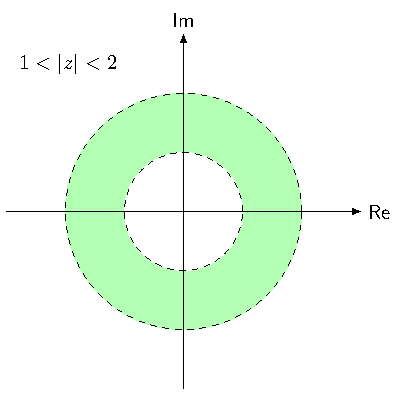
\includegraphics[scale=0.75]{annulus}\quad 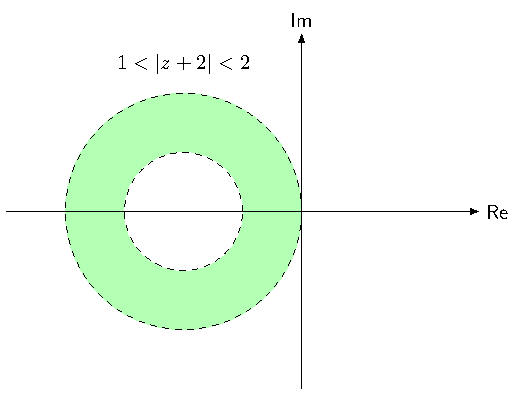
\includegraphics[scale=0.75]{annulus2}
\end{center}

\item[(c)] Write $z=x+iy$, then $z-i = x+i(y-1)$ and so
\begin{align*}
\set{z\in \C: 1 < \Im(z-i) <2 } &= \set{ x+iy \in \C : 1<y-1 <2 } \\
&= \set{x+iy \in \C: 2<y<3},
\end{align*}
which is the infinite horizontal band bounded by the lines $y=2$ and $y=3$.
\begin{center}
\oldincludegraphics[scale=0.75]{band}
\end{center}
\end{enumerate}
\end{answer}
\question 
\begin{parts}
\part Prove that for two nonzero complex numbers $z_1$ and $z_2$ we have
\[
\abs{z_1z_2} = \abs{z_1} \cdot \abs{z_2} \quad\text{ and }\quad \arg(z_1z_2)=\arg(z_1)\arg(z_2)
\]
(hint: write $z_1$ and $z_2$ in polar form).  Is it always true that $\Arg(z_1z_2)=\Arg(z_2)+\Arg(z_2)$?
\begin{answer}
Writing
\[
z_1=\polar{r_1}{\theta_1}\quad\text{and}\quad z_2=\polar{r_2}{\theta_2}
\]
we see that
\begin{align*}
z_1z_2&=r_1r_2 \left( \cos(\theta_1)\cos(\theta_2)-\sin(\theta_1)\sin(\theta_2) +i \left[ \cos(\theta_1)\sin(\theta_2)+\cos(\theta_2)\sin(\theta_1) \right] \right) \\
& = r_1r_2 \left( \cos(\theta_1+\theta_2)+i \sin(\theta_1+\theta_2) \right).
\end{align*}
Thus
\[
\abs{z_1z_2}=r_1r_2=\abs{z_1}\cdot \abs{z_2}\quad\text{and}\quad \arg(z_1z_2)=\theta_1+\theta_2=\arg(z_1)+\arg(z_2).
\]
It is not always true that $\Arg(z_1z_2)=\Arg(z_1)+\Arg(z_2)$.  Indeed, if $z_1=z_2=-1$ we have $\Arg (-1)=\pi$ but
\[
\Arg ((-1)(-1)) = \Arg (1) = 0.
\]
\end{answer}
\part Show that $\exp(z_1)\exp(z_2) = \exp(z_1+z_2)$.
\begin{answer}
With $z_1=x_1+iy_1$ and $z_2=x_2+iy_2$ a similar calculation to part (a) shows that
\begin{align*}
\exp(z_1)\exp(z_2) &= \polar{e^{x_1}}{y_1} \polar{e^{x_2}}{y_2} \\
 & = \polar{e^{x_1}e^{x_2}}{y_1+y_2} \\
 & = \polar{e^{x_1+x_2}}{y_1+y_2} = \exp(z_1+z_2).
\end{align*}
\end{answer}
\end{parts}
\question Write down the $3^{rd}$ roots of $-8$ in Cartesian form.
\begin{answer}
Writing $-8=\polar{8}{\pi}$, the three cubic roots are of the form $\polar{\sqrt[3]{8}}{(\pi+2k\pi)/3}$ for $k=0,1,2$.  In polar form, these are
\[
\polar{2}{\pi/3}, \quad \polar{2}{\pi} \quad\text{and}\quad\polar{2}{5\pi/3},
\]
or in Cartesian form $1+\sqrt{3},\ -2$ and $1-\sqrt{3}$ respectively.

\end{answer}

\question Find the values of $z$ for which $z^2+4iz-1=0$.  Which of these values lies inside the circle $C=\set{z \in \C: \abs{z}=1}$.
\begin{answer}
This is simply the usual quadratic formula: the roots of this polynomial are given by
\[
\frac{-4i\pm \sqrt{(4i)^2-4(1)(-1)}}{2} = \frac{-4i\pm i \sqrt{12}}{2} = i (-2 \pm  \sqrt{3}).
\]
To see which of these lies inside the circle $\abs{z}=1$, we examine the modulus and see that $\abs{i(-2 + \sqrt{3})} \approx 0.071<1$ and $\abs{i(-2-\sqrt{3})} \approx 1.93>1$. Thus only $i(-2+\sqrt{3})$ lies inside this circle.
\end{answer}


\question Show that $\Re (z) \leq \abs{ \Re (z)} \leq \abs{z}$ and $\abs{\Re (z)}+\abs{\Im (z)} \leq \sqrt{2} \abs{z}$.
\begin{answer}
The fact that $\Re (z) \leq \abs{ \Re (z)}$ is trivial.  Moreover,  writing $z=x+iy$ we see that
\[
\abs{\Re(z)} = \sqrt{x^2} \leq \sqrt{x^2+y^2}
\]
since $x^2 \leq x^2+y^2$ (and the square root function is increasing).

For the second inequality, note that with $z=x+iy$,
\begin{align*}
\left( \abs{\Re (z)}+\abs{\Im (z)} \right)^2 & = \left( \abs{x}+\abs{y} \right)^2 \\
& \leq \left( \abs{x}+\abs{y} \right)^2  + \overbrace{\left( \abs{x}-\abs{y} \right)^2}^{\geq 0}  \\
& = x^2+y^2+2\abs{xy} + x^2 + y^2 - 2\abs{xy} \\
& = 2(x^2+y^2) = 2 \abs{z}^2.
\end{align*}
Taking square roots of both sides yields the required inequality.
\end{answer}
\end{questions}

\setcounter{page}{1}
% !TEX root = exercises.tex

\exercisetitle{Exercise Sheet 1}

\begin{questions}
\question Use the triangle inequality $\abs{z_1-z_2} \leq \abs{z_1} + \abs{z_2}$ to prove the reverse triangle inequality:
\[
\abs{z_1-z_2} \geq \abs{\abs{z_1}-\abs{z_2}}
\]
\begin{answer}
The triangle inequality gives
\begin{align*}
\abs{z_1} & = \abs{z_1-z_2+z_2} \leq \abs{z_1-z_2} + \abs{z_2}  \\
\abs{z_2} & = \abs{z_2-z_1+z_1} \leq \abs{z_2-z_1} + \abs{z_1}\ (=\abs{z_1-z_2}+\abs{z_1}).
\end{align*}
Rearranging gives the two inequalities
\begin{align*}
\abs{z_1-z_2} & \geq \abs{z_1} - \abs{z_2} \\
\abs{z_1-z_2} & \geq \abs{z_2} - \abs{z_1},
\end{align*}
or in other words
\[
\abs{z_1-z_2} \geq \max \left( \abs{z_1}-\abs{z_2} , \abs{z_2} - \abs{z_1} \right) = \abs{\abs{z_1} - \abs{z_2} }.
\]
\end{answer}
\question Use the triangle and reverse triangle inequalities to show that for all $z$ on the circle $\abs{z}=2$, we have
\[
\abs{z+2} \leq 4 \text{ and } \abs{z-3+4i} \geq 3.
\]
Describe these inequalities geometrically.
\begin{answer}
If $\abs{z}=2$ then the triangle inequality ensures that
\[
\abs{z+2} \leq \abs{z}+2 = 4,
\]
and the backwards triangle inequality gives
\begin{align*}
\abs{z-3+4i} & = \abs{z-(3-4i)} \\
& \geq \abs{ \abs{z} - \abs{3-4i} } \\
& = \abs{2-5} = 3.
\end{align*}
Geometrically, these inequalities show respectively that the circle $\abs{z}=2$ is
\begin{itemize}
\item Contained in the disc with centre $-2$ and radius $4$ (i.e., the disc $\abs{z+2} \leq 4$), and
\item Outside of the disc with centre $3-4i$ and radius $3$.
\end{itemize}
\begin{center}
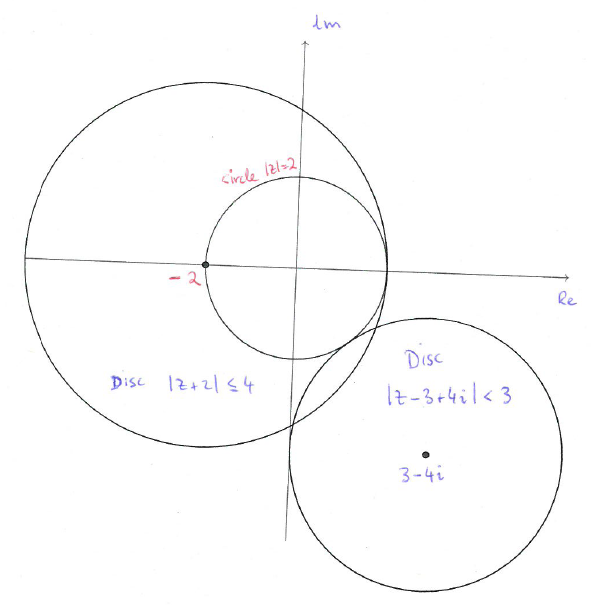
\includegraphics[scale=0.5]{ex1_q2}
\end{center}
\end{answer}
\question Use the triangle and reverse triangle inequalities to show that for all $z$ on the circle $\abs{z+3i}=3$ we have
\[
\abs{z-4} \leq 8,\quad \abs{z+5i}\geq 1 \text{ and } \abs{ \frac{z-4}{z+5i} } \leq 8.
\]
\begin{answer}

As with the previous question, the triangle inequality yields
\begin{align*}
\abs{z-4} & = \abs{z+3i-(3i+4)} \\
& \leq \abs{z+3i} + \abs{3i+4} \\
&=3+5=8.
\end{align*}
and the backwards triangle inequality yields
\begin{align*}
\abs{z+5i} & = \abs{z+3i+2i} \\
& \geq \abs{ \abs{z+3i} - \abs{2i} } \\
&=3-2=1.
\end{align*}
The third inequality is then obvious.
\end{answer}
\question Let $L$ be the line segment $[0,h]$ where $h \in \C$ and $\abs{h} < r$.  Show that if $\beta \in \C$ with $\abs{\beta}>2r$ and $z \in L$ then
\[
\abs{\frac{h-z}{\beta-z}} < \frac{\abs{h}}{r}.
\]
Do this using the reverse triangle inequality.  It can also be seen as follows.  Draw $L$ and two circles, both with centre $0$, $C_1$ with radius $r$ and $C_2$ with radius $2r$.  Why does $L$ lie inside $C_1$?  Where is $\beta$ on your diagram?  Why is $\abs{\beta-z}>r$?  If you can answer these three questions then the inequality should follow easily.
\begin{answer}

\begin{center}
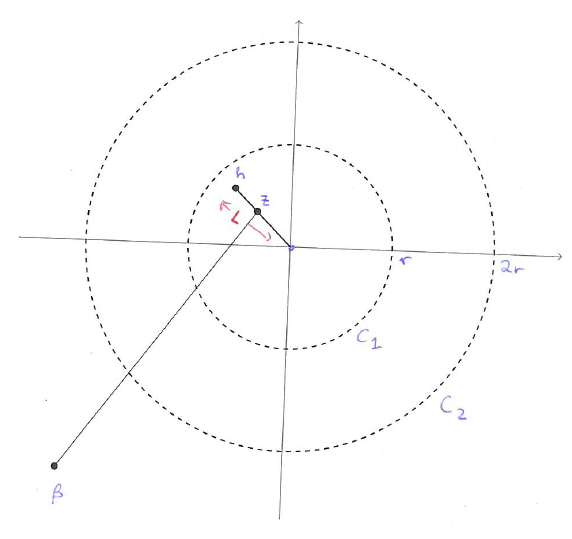
\includegraphics[scale=0.7]{ex1_q3}
\end{center}
Since $z$ lies on $L$, it is clear that $\abs{h-z} \leq \abs{h}$ (more formally, we can write $z=th$ for some $t$ with $0 \leq t \leq 1$, so that $\abs{h-z} = \abs{(1-t)h} = (1-t) \abs{h} \leq \abs{h}$).

The backwards triangle inequality, together with the fact that $\abs{z}<r<2r<\abs{\beta}$ gives
\begin{align*}
\abs{\beta - z} & \geq \abs{\abs{\beta}-\abs{z}} \\
& = \abs{\beta} - \abs{z} \\
&> 2r-r = r.
\end{align*}

Combining these two inequalities we see that
\begin{align*}
\abs{ \frac{h-z}{\beta - z} } &= \frac{\abs{h-z}}{\abs{\beta -z}} \\
 & \leq \frac{\abs{h}}{\abs{\beta - z}} \\
 & < \frac{\abs{h}}{r}.
\end{align*}

\end{answer}
\question The function $\mathbf{f}: \R^2 \to \R^2$ is defined by
$
\mathbf{f} (x,y)=(0,2y).
$
Show that the corresponding complex function $f:\C \to \C$ is
$
f(z) = z- \conj{z},
$
and that
\[
\lim_{h \to 0} \frac{f(z_0+h)-f(z_0)}{h}
\]
does not exist at any point $z_0 \in \C$.
\begin{answer}
The corresponding function is
\[
f(z) = f(x+iy) = i(2y) = i ( 2 \Im (z) ) = 2i \cdot \frac{z-\conj{z}}{2i} = z - \conj{z}.
\]
If $z_0 \in \C$ and $h \in \C \backslash \set{0}$ then
\[
\frac{f(z_0+h)-f(z_0)}{h} = \frac{(z_0+h)-\conj{(z_0+h)} - (z-\conj{z})}{h} = \frac{h-\conj{h}}{h} = 1- \frac{\conj{h}}{h}.
\]
Looking at restricted limits along the real and imaginary axes:
\[
1-\frac{\conj{h}}{h} \to \begin{cases}
1-1=0 & \text{ as } h \to 0, h \in \mathbb{R} \\
1-(-1)=2 & \text{ as } h \to 0, h \in i \R.
\end{cases}
\]
Since the restricted limits are not equal the (unrestricted) limit does not exist for any $z_0 \in \C$.

\end{answer}
\question Same as question 5 but with
\[
\mathbf{f}(x,y)=(x^2-y^2-x,2xy+y+1) \quad\text{ and }\quad f(z)=z^2-\conj{z}+i.
\]
\begin{answer}
This time, it is easier to start with the complex function $f$ and substitute $z=x+iy$:
\begin{align*}
f(z) & = z^2-\conj{z} + i \\
& = (x+iy)^2-(x-iy)+i \\
& = x^2-y^2+i2xy -x +iy +i \\
& = x^2-y^2-x + i \left( 2xy+y+1 \right),
\end{align*}
which shows that $f$ corresponds to the function $\mathbf{f}:\R^2 \to \R^2$ where
\[
\mathbf{f} (x,y) = \left( x^2-y^2-x, 2xy+y+1 \right).
\]
For $z_0 \in \C$ and $h \in \C \backslash \set{0}$ the difference quotient is
\begin{align*}
\frac{f(z_0+h)-f(z_0)}{h} & = \frac{(z_0+h)^2-\conj{(z_0+h)}+i-(z_0^2-\conj{z_0}+i )}{h} \\
& = h+2z_0-\frac{\conj{h}}{h}.
\end{align*}
Looking at some restricted limits:
\begin{align*}
\rlim{h \to 0}{h \in \R \backslash \set{0}} \frac{f(z_0+h)-f(z_0)}{h} & = 2z_0-1 \\
\rlim{h \to 0}{h \in i\R \backslash \set{0}} \frac{f(z_0+h)-f(z_0)}{h} & = 2z_0+1. \\
\end{align*}
These are not equal for any $z_0 \in \C$, so the unrestricted limit
\[
\lim_{h \to 0} \frac{f(z_0+h)-f(z_0)}{h}
\]
does not exist at any $z_0 \in \C$. 
\end{answer}
\question Let $f:\C \to \C$ be defined by $f(z) = \abs{z}^2$.  Show that $f$ is differentiable at $z=0$ and nowhere else.
\begin{answer}
Since $\abs{z}^2 = z \conj{z}$,
\begin{align*}
\frac{f(z_0+h)-f(z_0)}{h} &= \frac{(z_0+h)\conj{(z_0+h)}-z_0\conj{z_0}}{h} \\
& = \frac{z_0\conj{h}+h\conj{z_0}+h\conj{h}}{h} \\
&= z_0\frac{\conj{h}}{h} + \conj{z_0}+\conj{h} \\
& \longrightarrow
\begin{cases}
2z_0 & \text{ as }h \to 0,\ h \in \R \backslash \set{0} \\
0 & \text{ as } h \to 0, h \in i\R \backslash \set{0}.
\end{cases}
\end{align*}
For $z_0 \neq 0$, the restricted limits are not equal, hence the unrestricted limit does not exist and so $f$ is not differentiable at any point $z_0 \in \C \backslash \set{0}$.

At $z_0=0$, we have
\[
\lim_{h \to 0} \frac{f(0+h)-f(0)}{h} = \lim_{h \to 0} \conj{h} = 0,
\]
so that $f$ is differentiable at $0$ with $f'(0)=0$.
\end{answer}
\question Use the rules of differentiation to find the derivatives of the following functions:
\begin{parts}
\part $f(z) = \left( z^2+4 \right)^3$
\part $g(z) = \dfrac{z+i}{z-i}$.
\end{parts}
Find the values of $f'(i)$ and $g'(1)$.
\begin{answer}
\begin{parts}
\part Since $f$ is the composition of holomorphic functions, we can use the chain rule to find $f'(z)$:
\[
f'(z) = 3 ( z^2+4)^2(2z) = 6z(z^2+4)^2 \quad \text{ for all } z \in \C,
\]
and
\[
f'(i) = 6i (i^2+4)^2 = 6i(3)^2 = 54i.
\]
\part Since the functions $z \mapsto z\pm i$ are holomorphic on $\C$, $g$ is holomorphic on $\C \backslash \set{i}$, and the quotient rule gives
\[
g'(z) = \frac{(z-i)(1)-(z+i)(1)}{(z-i)^2} = \frac{-2i}{(z-i)^2}
\]
for all $z \in \C \backslash \set{i}$.  Hence
\[
g'(1) = \frac{-2i}{(1-i)^2} = \frac{-2i}{-2i} = 1.
\]
\end{parts}
\end{answer}

\end{questions}

\setcounter{page}{1}
% !TEX root = exercises.tex

\exercisetitle{Exercise Sheet 2}

\begin{questions}
\question For each function $f$ below, write $f$ in the form
\[
f(z) = f(x+iy) = u(x,y)+iv(x,y)
\]
and determine whether or not the Cauchy-Riemann equations are satisfied:
\[ (a)\ f(z) = \exp(i\ \conj{z})\quad  (b)\ f(z) = z + \dfrac{1}{z}\quad (c)\ f(z)=z^3.\]

In the cases where $f$ is differentiable, find the derivative of $f$ both using the rules of differentiation and using the Cauchy-Riemann equations.
\begin{answer}
\begin{parts}
\part We have 
\[
f(x+iy) = \exp (i (x-iy) ) = \exp (y+ix ) = \underbrace{e^{y} \cos (x) }_{u(x,y)} + i \underbrace{e^{y} \sin (x)}_{v(x,y)}.
\]
The corresponding partial derivatives are
\begin{align*}
\pd{u}{x} & = -e^{y} \sin(x) & \pd{v}{y} = e^{y} \sin(x) \\
\pd{u}{y} & = e^{y} \cos (x) &  \pd{v}{x} = e^{y} \cos (x).
\end{align*}
The Cauchy Riemann Equations are satisfied at a point $x+iy \in \C$ if and only if both
\[
e^y \sin(x) = -e^{y} \sin(x)\quad\text{and}\quad e^{y} \cos (x) = - e^{y} \cos (x).
\]
Since $e^y$ is never zero, this can only occur if $\sin(x)=\cos(x)=0$, which is impossible.  

\part For all $x +iy \in \C \backslash \set{0}$, 
\begin{align*}
f(x+iy) &= (x+iy) + \frac{1}{x+iy} \\
& = (x+iy) + \frac{x-iy}{x^2+y^2} \\
& = \underbrace{\left( x+ \frac{x}{x^2+y^2}  \right)}_{u(x,y)} + i \underbrace{\left( y-\frac{y}{x^2+y^2} \right) }_{v(x,y)}
\end{align*}
and the corresponding partial derivatives are
\begin{align*}
& \pd{u}{x} = 1+\frac{y^2-x^2}{(x^2+y^2)^2} && \pd{u}{y} = \frac{-2xy}{(x^2+y^2)^2} \\
& \pd{v}{x} = \frac{2xy}{(x^2+y^2)^2} && \pd{v}{y} = 1 - \frac{x^2-y^2}{(x^2+y^2)^2}.
\end{align*}
Hence the Cauchy Riemann equations are satisfied at every $x+iy \in \C \backslash \set{0}$.  Using the Cauchy Riemann equations to find the derivative of $f$, we get
\begin{align*}
f'(x+iy ) & = \pd{u}{x} + i \pd{v}{x} \\
& = \left( 1+\frac{y^2-x^2}{(x^2+y^2)^2} \right) + i \left( \frac{2xy}{(x^2+y^2)^2} \right) \\
& = 1 + \frac{y^2-x^2+i2xy}{(x^2+y^2)^2} \\
& = 1 - \frac{x^2-y^2-i2xy}{(x^2+y^2)^2} \\
& = 1 - \frac{(x-iy)^2}{\left[ (x+iy)(x-iy) \right]^2} \\
& = 1 - \frac{1}{(x+iy)^2} = 1- \frac{1}{z^2},
\end{align*}
which agrees with the derivative of $f$ obtained from the rules of differentiation.
\part This time
\[
u(x,y) = x^3-3xy^2 \quad\text{and}\quad v(x,y)=3x^2y-y^3
\]
hence for all $x+iy \in \C$
\[
\pd{u}{x} = 3x^2-3y^2=\pd{v}{y} \quad\text{and}\quad \pd{u}{y}=-6xy=-\pd{v}{x}.
\]
Thus
\[
f'(x+iy) = \pd{u}{x} (x,y)+i\pd{v}{y}(x,y) = 3x^2-3y^2+i(6xy) = 3 \left( (x^2-y^2)+i(2xy) \right) = 3(x+iy)^2
\]
which agrees with the derivative obtained from the Chain Rule: $f'(z)=3z^2$.
\end{parts}
\end{answer}

\question Show that the Cauchy-Riemann equations are satisfied by the function $f$ defined on the open upper half plane $H_+=\set{ z \in \C: \Im (z) > 0 }$ by
\[
f(x+iy) = u(x,y)+iv(x,y) = \log \left( \sqrt{ x^2+y^2 } \right) + i \left( \frac{\pi}{2} - \arctan \left( \frac{x}{y} \right) \right).
\]
Assuming that $f$ is indeed holomorphic on $H_+$, show that
\[
f'(x+iy) = \frac{1}{x+iy}\quad \text{i.e., that }\quad f'(z) = \frac{1}{z}.
\]
\begin{answer}
We have
\begin{align*}
\pd{u}{x} &= \log' \left( \sqrt{ x^2+y^2 } \right) \cdot \pd{}{x} \left[ \sqrt{x^2+y^2} \right] \\
& = \frac{1}{\sqrt{x^2+y^2}} \cdot \frac{1}{2} (x^2+y^2)^{-\frac{1}{2}}(2x) \\
&=  \frac{x}{x^2+y^2}
\shortintertext{ and similarly }
\pd{u}{y} & = \frac{y}{x^2+y^2}.\\
\intertext{For the partial derivatives of $v$, we have}
\pd{v}{x} & = - \arctan ' \left( \frac{x}{y} \right) \cdot \pd{}{x} \left[ \frac{x}{y} \right] \\
& = \frac{-1}{(1+(\frac{x}{y})^2)} \cdot \frac{1}{y} \\
& = \frac{-1}{y+\frac{x^2}{y}} = \frac{-y}{x^2+y^2} \\
\shortintertext{and }
\pd{v}{y} & = - \arctan ' \left( \frac{x}{y} \right) \cdot \pd{}{y} \left[ \frac{x}{y} \right] \\
& = \frac{-1}{(1+(\frac{x}{y})^2} \cdot \frac{-x}{y^2} \\
& = \frac{x}{x^2+y^2}.
\end{align*}
Thus the Cauchy-Riemann equations 
\[
\pd{u}{x} = \pd{v}{y},\quad \pd{u}{y} = - \pd{v}{x}
\]
are satisfied everywhere in $H_+$.  Assuming moreover that $f$ is holomorphic on $H_+$, the derivative of $f$ is thus
\begin{align*}
f'(x+iy) & = \pd{u}{x} + i \pd{v}{x} \\
& = \frac{x}{x^2+y^2}+i \frac{-y}{x^2+y^2} \\
& = \frac{x-iy}{(x+iy)(x-iy)} = \frac{1}{x+iy}
\end{align*}
for all $x+iy \in H_+$ as required.
\end{answer}

\question Describe the geometric effect of applying the functions:
\begin{parts}
\part $f(z) = \dfrac{1}{z}$ to a small disc centred at $1-i$, and 
\part $g(z) = \exp(2iz)$ to a small disc centred at $\frac{\pi}{4}+i$.
\end{parts}
\begin{answer}
For a function $f$ that is holomorphic at a point $z_0$, we know that a small disc centred at $z_0$ is approximately mapped to a small disc centred at $f(z_0)$, and is scaled by a factor of $\abs{f'(z_0)}$ and rotated by an angle of $\arg (f'(z_0))$ about the point $f(z_0)$.
\begin{parts}
\part In this example, $f(1-i)=\dfrac{1}{1-i}=\dfrac{1}{2}+\dfrac{i}{2}$, so a small disc centred at $1-i$ is approximately mapped to a small disc centred at $\dfrac{1}{2}+\dfrac{i}{2}$.  Since $f'(z) = -\dfrac{1}{z^2}$ for all $z \in \C \backslash \set{0}$, we have $f'(i)=-\dfrac{1}{(1-i)^2} = \frac{i}{2}$.  Thus the disc is scaled by a factor of $\frac{1}{2}$ and rotated by an angle of $\frac{\pi}{2}$ about $\dfrac{1}{2}-\dfrac{i}{2}$.
\part Mapped to a disc centred at $g(\frac{\pi}{4}+i)=e^{-2}i$, scaled by a factor of $2e^{-2}$ and rotated by an angle of $\pi$ about this point (clockwise or anticlockwise; it doesn't matter this time).
\end{parts}
\end{answer}
\question  The \emph{set} of points $L=[0,1-2i]$ is a line segment.  It is also a \emph{path} because we have a parametrisation given by  $\gamma:[0,1] \to \C,\ \gamma(t) = (1-2i)t.$  Use this parametrisation to evaluate the integral
\[
\int_L \left( \Im (z) + 3i \right)\ dz.
\]
\begin{answer}

We have
\begin{align*}
\int_{\Gamma} ( \Im (z) + 3i )\ dz & = \int_0^1 \left( \Im ( \gamma (t) ) +3i \right) \gamma' (t)\ dt \\
& = \int_0^1 \left( -2t + 3i \right) (1-2i)\ dt \\
& = (1-2i) \int_0^1 (-2t +3i)\ dt \\
& = (1-2i) \left[ - t^2 +3it \right]_0^1 \\
& = (1-2i)(-1+3i) = 5 + 5i.
\end{align*}

\end{answer}
\question Find the value of
\[
\int_{\Gamma_1} f(z)\ dz \text{ and } \int_{\Gamma_2} f(z)\ dz,
\]
where $f(z) = 3 \conj{z}$, $\Gamma_1$ is the straight line path from $0$ to $-i$ and $\Gamma_2$ is the straight line path from $1-i$ to $1+i$.
\begin{answer}
For the path $\Gamma_1$ we use the parametrisation $\gamma_1:[0,1] \to \C$, $\gamma_1 (t) = -it.$  Then $\gamma_1'(t)=-i$ and $f(\gamma_1(t)) = 3it$.  Hence
\[
\int_{\Gamma_1} f = \int_0^1 (3it)(-i)dt = \int_0^1 3t\ dt = \frac{3}{2}.
\]
Parametrise $\Gamma_2$ with $\gamma_2:[0,1] \to \C$, where
\[
\gamma_2 (t) = (1-i) + t \left[ 1+i-(1-i) \right] = 1+i(2t-1).
\]
We get
\[
\int_{\Gamma_2} f = 6i.
\]
\end{answer}





\question Fix a point $z_0 \in \C$ and define a complex function $f$ via
\[
f(z) = (z-z_0)^n
\]
where $n \in \mathbb{Z}$.  Find the value of
\[
\int_{\Gamma} f(z)\ dz,
\]
where $\Gamma$ is the circle with centre $z_0$ and radius $r>0$, traversed in the anticlockwise direction (use the parametrisation $\gamma:[0,2\pi] \to \C, \ \gamma (t) = z_0 + r \left( \cos (t) + i \sin (t) \right)$).  Do this separately for the cases $n=-1$ and $n \neq -1$.

(Hint: for the case $n \neq -1$, you need to show that
\[
\frac{d}{dt} \left[ \left( \cos(t)+i \sin(t) \right)^{n+1} \right] = i(n+1) \left( \cos(t)+i \sin(t) \right)^{n+1}
\]
and then use the (real) Fundamental Theorem of Calculus).
\begin{answer}
Following the hint, we first note that
\begin{align*}
\frac{d}{dt} \left[ \left( \cos(t)+i \sin(t) \right)^{n+1} \right] & = (n+1) \left( \cos(t)+i \sin(t) \right)^{n} \left( - \sin (t)+i \cos(t) \right) \\
& = (n+1) \left( \cos(t)+i \sin(t) \right)^{n} i \left( \cos(t)+i \sin(t) \right) \\
& = i(n+1) \left( \cos(t)+i \sin(t) \right)^{n+1}.
\end{align*}
We have
\[
f(\gamma(t))=\left( \gamma(t)-z_0 \right)^n = r^n \left( \cos (t)+i \sin (t) \right)^n,\quad \gamma'(t) = i r\left( \cos(t) + i \sin (t) \right).
\]
Hence for $n \neq -1$,
\begin{align*}
\int_{\Gamma} (z-z_0)^n & = \int_0^{2\pi} i r^{n+1} \left( \cos(t) + i \sin (t) \right)^{n+1}\ dt &&\\
& = \frac{r^{n+1}}{n+1} \int_0^{2\pi} \frac{d}{dt} \left[ \left( \cos(t) + i \sin (t) \right)^{n+1} \right]\ dt && \\
& = \frac{r^{n+1}}{n+1} \left[ \left( \cos(t) + i \sin (t) \right)^{n+1} \right]_0^{2\pi} && \text{ by FTC }\\
& = \frac{r^{n+1}}{n+1} \left[ 1+0i-(1+0i) \right] = 0 &&.
\end{align*}
If $n=-1$ then
\[
\int_{\Gamma} (z- z_0)^{-1} = \int_0^{2\pi} \frac{1}{r(\cos(t)+i\sin(t) )} \cdot ir (\cos(t)+i\sin(t) )\ dt =  \int_0^{2\pi} i\ dt = i2\pi.
\]


\end{answer}
\question Let $f,g:U \to \C$ be continuous, and let $\Gamma$ be a smooth path contained in $U$ parametrised by $\gamma:[a,b] \to \C$.  Prove that
\begin{parts}
\part for every constant $\alpha \in \C$ we have $\displaystyle \int_{\Gamma} ( f + \alpha g ) = \int_{\Gamma} f + \alpha \int_{\Gamma} g$, and
\part if $\tilde{\Gamma}$ denotes the reverse of $\Gamma$, we have $\displaystyle \int_{\tilde{\Gamma}} f = - \int_{\Gamma} f$.  As a hint, parametrise $\tilde{\Gamma}$ using $\tilde{\gamma}:[a,b] \to \C$, $\tilde{\gamma}(t)=(a+b-t)$, and use the substitution $s=a+b-t$.
\end{parts}
\begin{answer}
\begin{parts}
\part 
\begin{align*}
\int_{\Gamma} ( f + \alpha g ) & = \int_a^b (f + \alpha g )(\gamma(t)) \gamma'(t)\ dt \\
& = \int_a^b \left( f(\gamma(t)) + \alpha g(\gamma(t)) \right) \gamma' (t)\ dt \\
& = \int_a^b \left( f(\gamma(t)) \gamma'(t) + \alpha g (\gamma(t))\gamma'(t) \right)\ dt 
\end{align*}
Then using linearity of the real integral this becomes
\[
\int_a^b f(\gamma(t)) \gamma'(t)\ dt + \alpha \int_a^b g (\gamma(t))\gamma'(t)\ dt = \int_{\Gamma} f + \alpha \int_{\Gamma} g.
\]
\part Following the hint,
\begin{align*}
\int_{\tilde{\Gamma}} f & = \int_a^b f ( \tilde{\gamma} (t) ) \tilde{\gamma}' (t)\ dt \\
& = \int_a^b f ( \gamma(a+b-t) ) \left( - \gamma '(a+b-t) \right)\ dt
\end{align*}
and using the substitution $s=a+b-t$, we have $ds=-dt$ and the limits are reversed, so the above becomes
\begin{align*}
\int_b^a f ( \gamma (s) ) \left( - \gamma'(s) \right) (- ds) & = \int_b^a f (\gamma(s))\gamma'(s)\ ds \\ 
& = - \int_a^b f(\gamma(s)) \gamma'(s)\ ds \\
& = - \int_{\Gamma} f.
\end{align*}
\end{parts}
\end{answer}
\end{questions}
\setcounter{page}{1}
% !TEX root = exercises.tex

\exercisetitle{Exercise Sheet 3}

\begin{questions}
\question Find antiderivatives for the following functions:
\begin{parts}
\part $f(z) = \alpha + \beta(z-z_0)$,
\part $f(z) = (z-z_0)^n$,
\end{parts}
where $\alpha,\beta$ and $z_0 \in \C$ are constants and $n$ is an integer, $n \neq -1$.  Does $g(z)=(z-z_0)^{-1}$ have an antiderivative on $\C \backslash \set{z_0}$?  Question 6 on Exercise Sheet 2 may help here.  
\begin{answer}
\begin{enumerate}
\item[(a)] An antiderivative for $f$ on $\C$ is given by $F:\C \to \C$ where
\[
F(z) = \alpha z + \frac{1}{2} \beta z^2 - \beta z_0 z,
\]
since
\[
F'(z) = \alpha + ( \frac{1}{2} \beta ) (2z) - \beta z_0 = \alpha + \beta(z-z_0) = f(z)
\]
for all $z \in \C$.
\item[(b)] For $n \geq 0$ (respectively $n<-1$), and antiderivative for $f$ on $\C$ (respectively $\C \backslash \set{z_0}$) is given by $F$ where
\[
F(z) = \frac{1}{n+1} (z-z_0)^{n+1}.
\]
\end{enumerate}
The function $g$ does not have an antiderivative on $\C \backslash \set{0}$, since if it did, the Fundamental Theorem of Calculus would imply that
\[
\int_{\Gamma} g = 0
\]
where $\Gamma$ is the anticlockwise circular contour with centre $0$ and radius $1$.  We know from Exercise Sheet 2 that this integral has the value $2\pi i \neq 0$.
\end{answer}
\question Evaluate the following contour integrals:
\[
\int_{\mathcal{C}} z^3 \quad \text{ and } \quad \int_{\mathcal{C}} \frac{1}{z^2}
\]
along $\mathcal{C}$ where $\mathcal{C}$ is
\begin{parts}
\part any contour from $i$ to $-2$, and
\part any closed contour.
\end{parts}
For the second integral, you may assume that $\mathcal{C}$ does not contain $0$.
\begin{answer}
An antiderivative for $f(z) = z^3$ on $\C$ is given by the function $F$ with $F(z) = \frac{1}{4} z^4$.  Hence by the Fundamental Theorem of Calculus we have
\[
\int_{\mathcal{C}} z^3 = F(-2) - F(i) = \frac{1}{4} (-2)^4-\frac{1}{4} (i)^4 = \frac{15}{4}
\]
where $\mathcal{C}$ is any contour from $i$ to $-2$, and 
\[
\int_{\mathcal{C}} z^3 = 0
\]
when $\mathcal{C}$ is any closed contour.

Similarly $G(z) = \frac{-1}{z}$ is an antiderivative for $g(z) = \frac{1}{z}$ on $\C \backslash \set{0}$, and $\C \backslash \set{0}$ is a region in $\C$ (it is open and connected).  Hence by the Fundamental Theorem of Calculus we have
\[
\int_{\mathcal{C}} \frac{1}{z} = G(-2)-G(i) = \frac{-1}{-2} - \frac{-1}{i} = \frac{1}{2} -i
\]
for any contour $\mathcal{C}$ in $\C \backslash \set{0}$ from $i$ to $-2$, and
\[
\int_{\mathcal{C}} \frac{1}{z} =0
\]
for any closed contour $\mathcal{C}$ in $\C \backslash \set{0}$.

\end{answer}
\question Let $U$ be a region in $\C$ and let $f:U \to \C$ be holomorphic on $U$ with $f(z)$ real-valued for all $z \in U$.  Prove that $f$ is constant.
\begin{answer}
Write $f$ in the form
\[
f(x+iy)=u(x,y)+iv(x,y)
\]
where $u$ and $v$ are real-valued functions of two real variables.
If $f(z)$ is real valued then $v(x,y)=0$ on $U$, hence $\dfrac{\partial v }{\partial x} = \dfrac{\partial v}{\partial y}=0$ on $U$.

Since $f$ is holomorphic, $u$ and $v$ satisfy the Cauchy-Riemann equations, it follows that $\dfrac{\partial u}{\partial x} = \dfrac{\partial u}{\partial y}=0$ on $U$, hence
\[
f' = \frac{\partial u}{\partial x} + i \frac{\partial v}{\partial x} = 0
\]
on $U$. 

Since $U$ is connected, this implies that $f$ is constant by the Fundamental Theorem of Calculus.
\end{answer}


\question Find an upper estimate for
\[
\int_{\mathcal{C}} \frac{1}{1+z^4},
\]
where $\mathcal{C}$ is the upper semicircular contour from $R$ to $-R$ given by $\gamma:[0,\pi] \to \C$, $\gamma (t) = R \cos(t)+iR \sin (t)$.

\begin{answer}
We shall do this using the Estimation Lemma.  In order to apply the Lemma, we need to find $\ell{\Gamma}$ and an upper bound for $\abs{\frac{1}{1+z^4}}$ along $\mathcal{C}$.  Now, we know that
\[
\gamma '(t) = -R \sin(t) +i R \cos(t)
\]
with modulus
\[
\abs{\gamma'(t)} = \sqrt{ (-R\sin(t))^2+(R\cos(t))^2} = \sqrt{R^2(\sin^2(t)+\cos^2(t))} = R
\]
for all $t \in [0,\pi]$.  Hence the length of $\mathcal{C}$ is given by
\[
\ell(\mathcal{C})=\int_0^{\pi} \abs{\gamma'(t)} dt = \int_0^{\pi} R \ dt =\pi R.
\] 

Moreover, if $z$ lies in $\mathcal{C}$ then $z=\gamma(t)$ for some $t \in [0,\pi]$, hence
\[
\abs{z} = \abs{\gamma(t)} = \sqrt{(R\cos(t))^2+(R\sin(t))^2} = R.
\]
Using the backwards triangle inequality, for all $z \in \mathcal{C}$ we have
\[
\abs{1+z^4} \geq \abs{1-\abs{-z^4}} = \abs{1-R^4} = R^4-1
\]
(since $R>1$), and so
\[
\abs{\frac{1}{1+z^4}} \leq \frac{1}{R^4-1}
\]
whenever $z \in \mathcal{C}$.  Thus the Estimation Lemma tells us that
\[
\abs{\int_{\mathcal{C}} \frac{1}{1+z^4}} \leq \frac{1}{R^4-1} \cdot (\pi R) = \frac{\pi R}{R^4-1},
\]
so that $\pi R/(R^4-1)$ is an upper estimate for the integral $\int_{\mathcal{C}} 1/(1+z^4)$.


\end{answer}


\question Show that for all points $z$ on the circle $\set{z: \abs{z}=5}$ we have
\[
\abs{z-7} \leq 12 \quad \text{and}\quad \abs{\conj{z}+8} \geq 3,
\]
and use this to find an upper estimate for the integral
\[
\int_S \frac{z-7}{(\conj{z}+8)^2}\ dz
\]
where $S$ is the same circle oriented anticlockwise.

\begin{answer}
The first two inequalities can be shown using the triangle and backwards triangle inequalities respectively.  Using these, we have 
\[
\abs{\frac{z-7}{(\conj{z}+8)^2}} = \frac{\abs{z-7}}{\abs{\conj{z}+8}^2} \leq \frac{12}{3^2} = \frac{4}{3}
\]
for all $z \in S$.  The length of $S$ is $10\pi$, and so by the Estimation Lemma, we get the upper estimate
\[
\abs{
\int_S \frac{z-7}{(\conj{z}+8)^2}\ dz
}
\leq \frac{4}{3} \cdot 10\pi = \frac{40\pi}{3}.
\]
\end{answer}

\question Let $S_a$ be the anticlockwise square contour with corners at $\pm a(1+i),\pm a(1-i)$ where $a>0$.  Show that if $z \in S_a$ then
\[
\frac{1}{\abs{z}} \leq \frac{1}{a} \]
and hence
\[ \abs{ \int_{S_a} \frac{1}{z} dz } \leq 8,
\]
for all $a>0$.

\begin{answer}
Note that this square lies in the region outside the circle $\set{z:\C: \abs{z}=a}$.
\begin{center}
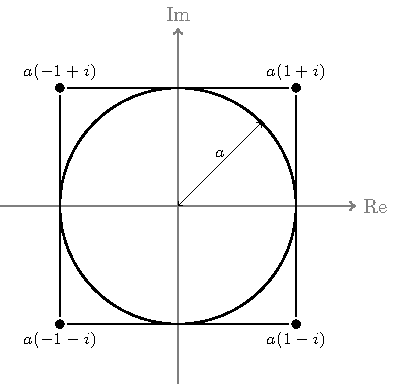
\includegraphics[scale=1]{squareandcircle}
\end{center}
Any point $z$ outside of this circle has modulus $\abs{z} \geq a$; in particular, this is true for any $z \in S_a$.  Hence for all such $z$, $\abs{\dfrac{1}{z}} \leq \dfrac{1}{a}$.

The length of each straight edge of $S_a$ is $2a$, and hence $\ell (S_a) = 8a$.  The Estimation Lemma then gives the required inequality.
\end{answer}

\question Prove each of the following:
\begin{parts}
\part For $z_0$ and $h$ in $\C$ we have $\displaystyle \int_{[z_0,z_0+h]} 1\ dz = h$.
\part For $f:U \to \C$ and $z_0 \in U$, $f(z_0) = \displaystyle \frac{1}{h} \int_{[z_1,z_1+h]} f(z_0)\ dz$.
\part If $\alpha$ is a complex number  and $M$ a fixed real number with $\abs{\alpha} \leq \epsilon M$ for all $\epsilon >0$ then $\alpha=0$.
\end{parts}
\begin{answer}
\begin{parts}
\part Using the parametrisation $\gamma:[0,1] \to \C$, $\gamma(t)=z_0+t(z_0+h-z_0) = z_0+th$, we have
$\gamma'(t)=h$ and $f(\gamma(t))=1$.  Hence
\[
\int_{[z_0,z_0+h]} 1dz = \int_0^1 f(\gamma(t)) \gamma '(t)\ dt = \int_0^1 1 (h) \ dt = h.
\]
Alternatively, using the antiderivative $F(z)=z$ for $f$, we have (by the Fundamental Theorem of Calculus)
\[
\int_{[z_0,z_0+h]} 1dz = F(z_0+h)-F(z_0)=z_0+h-z_0=h.
\]
\part Since $f(z_0)$ is a constant we have
\[
\frac{1}{h} \int_{[z_1,z_1+h]} f(z_0) dz = \frac{1}{h} f(z_0) \int_{[z_1,z_1+h]} 1 dz = \frac{1}{h} f(z_0) h = f(z_0)
\]
by the previous part.
\part Suppose that $\alpha \neq 0$.  Then $\abs{\alpha}>0$ (since for $z \in \C$ we have $\abs{z}=0$ if and only if $z=0$).  Setting $\epsilon = \abs{\alpha}/2M$ we have $\epsilon >0$, which implies that
\[
\abs{\alpha} \leq \epsilon M =  \frac{\abs{\alpha}}{2M} \cdot M = \frac{\abs{\alpha}}{2}.
\]
But this is only possible if $\abs{\alpha} =0$, a contradiction.  Hence $\abs{\alpha}=0$ and so $\alpha=0$.
\end{parts}
\end{answer}


\begin{comment}
\newpage


\question All of the proofs that have been done in lectures are examinable.  As some of these are quite long, you should be prepared to answer questions of the following format, where an outline of the proof is presented in the form of a series of statements.  For each numbered statement, provide a brief comment that explains or justifies it.  

\noindent{\bf Theorem (Cauchy's Theorem for a Triangle) } Let $\mathcal{R}$ be a simply connected region, $f$ a function that is holomorphic on $\mathcal{R}$ and let $T$ be a triangle in $\mathcal{R}$ with boundary $\partial T$.  Then
\[
\int_{\partial T} f =0.
\]
\medskip
{\bf Proof } 
There exists a nested sequence of triangles $\{ T_n \}$ such that
\[
\left( \frac{1}{4} \right)^n \left| \int_{\partial T} f \right| \leq \left| \int_{\partial T_n} f \right| \quad\text{ and }\quad \ell (\partial T_n ) = \left( \frac{1}{2} \right)^n \ell ( \partial T),
\]
and there is a point $z_0 \in \mathcal{R}$ with $z_0 \in T_n$ for all $n$.
\begin{enumerate}
\item[(1)] Given $\varepsilon >0$ there exists $\delta >0$ such that
\[
|z-z_0| < \delta \Longrightarrow \left| f(z)-f(z_0)-(z-z_0)f'(z_0) \right| \leq \varepsilon |z-z_0|
\]
\begin{answer}
Since $f$ is holomorphic on $\mathcal{R}$, $f$ is differentiable at $z_0$ and hence
\[
\lim_{z \to z_0} \frac{f(z)-f(z_0)}{z-z_0}
\]
exists and is equal to $f'(z_0)$.  

By the definition of a limit, given $\varepsilon>0$ there is $\delta >0$ such that
\begin{align*}
0< | z-z_0 | < \delta &\Rightarrow \left| \frac{f(z)-f(z_0)}{z-z_0}-f'(z_0) \right| < \varepsilon \\
& \Rightarrow \left| \frac{f(z)-f(z_0)-(z-z_0)f'(z_0)}{z-z_0} \right| < \varepsilon \\
& \Rightarrow \left| f(z)-f(z_0)-(z-z_0)f'(z_0) \right| < \varepsilon |z-z_0|.
\end{align*}
Finally, if $z=z_0$ then both sides of the final inequality are zero, which shows (1).
\end{answer}
\item[(2)] There exists $n$ such that $\ell ( \partial T_n) < \delta$ and $T_n \subset D(z_0;\delta)$.
\begin{answer}
Since $\ell ( \partial T)$ is fixed, we can choose $n$ large enough so that $\ell ( \partial T)/2^n < \delta$.  By the first (un-numbered) statement, for any such $n$ we have $\ell ( \partial T_n) < \delta$.

Since $z_0$ lies inside $T_n$, the distance from $z_0$ to any point on $\partial T_n$ is less than $\ell ( \partial T_n)$.
\end{answer}

\item[(3)]  For $z \in \partial T_n$
\[
\left| f(z)-f(z_0)-f'(z_0)(z-z_0) \right|< \epsilon \ell ( \partial T_n).
\]
\begin{answer}
By (2), for $z \in \partial T_n$ we have $|z-z_0| < \delta$, hence by (1), for all such $z$ we have
\[
\left| f(z)-f(z_0)-f'(z_0)(z-z_0) \right| \leq \varepsilon | z-z_0 | < \varepsilon \delta < \varepsilon \ell ( \partial T_n )
\]
the final inequality following from (2).
\end{answer}
\item[(4)] \hfil $\displaystyle \int_{\partial T_n} f(z)\ dz = \int_{\partial T_n} \left( f(z)-f(z_0)-f'(z_0)(z-z_0) \right)\ dz$\hfil
\begin{answer}
The (linear) function $z \mapsto f(z_0)+(z-z_0)f'(z_0)$ has an antiderivative on $\mathbb{C}$, and since $\partial T_n$ is a closed path,
\[
\int_{\partial T_n} f(z_0)+(z-z_0)f'(z_0)\ dz =0,
\]
so (4) follows from linearity of path integrals.
\end{answer}
\item[(5)]  \hfil $  \displaystyle \left| \int_{\partial T_n} f \right| \leq \varepsilon\ \left[\ell (\partial T_n ) \right]^2$ \hfil
\begin{answer}
The function $z \mapsto f(z) - f(z_0)-(z-z_0)f'(z_0)$ is bounded above on $\partial T_n$ by $ \varepsilon \ell ( \partial T_n )$ by (3), hence by the Estimation Lemma,
\[
\left| \int_{\partial T_n} f(z) - f(z_0)-(z-z_0)f'(z_0)\ dz \right| \leq \varepsilon \ell ( \partial T_n ) \cdot \ell ( \partial T_n ).
\]
Together with (4), this yields (5).
\end{answer}
\item[(6)] 
\hfil
$
 \displaystyle \left( \frac{1}{4} \right)^n \left| \int_{\partial T} f \right| \leq \left| \int_{\partial T_n} f \right| \leq \varepsilon\ \left[\ell (\partial T_n ) \right]^2 \leq \varepsilon \left(\frac{1}{4} \right)^n \left[ \ell ( \partial T) \right]^2.
$ \hfil
\begin{answer}
The first and last inequalities are given in the first (un-numbered) statement, the second was shown in (4).
\end{answer}
\item[(7)]\hfil $\displaystyle \int_{\partial T} f = 0 .$\hfil
\begin{answer}
By (6) we have
\[
\left| \int_{\partial T} f \right| \leq \varepsilon \left[ \ell ( \partial T ) \right]^2
\]
for all $\varepsilon >0$.  Since $\ell ( \partial T )$ is a constant, (7) follows.
\end{answer}
\end{enumerate}
\end{comment}



\end{questions}
\setcounter{page}{1}
% !TEX root = exercises.tex

\exercisetitle{Exercise Sheet 4}

\begin{questions}
\question Express each of the following complex numbers in Cartesian form $a+ib$:
\[
(a)\ \Log (i), \quad (b)\ \Log (ie)\quad (c)\  \Log (-1-i\sqrt{3}).
\]
\begin{answer}
Using $\Log (z) = \log \abs{z} + i \Arg (z)$,
\begin{align*}
\Log(i) & = \log \abs{i} + i \Arg (i) = \log(1)+i\frac{\pi}{2} = i\frac{\pi}{2}.\\
\Log (ie) &= \log(e)+i\frac{\pi}{2}  = 1 + i \frac{\pi}{2} \\
 \Log (-1-i\sqrt{3}) & =  \log (\sqrt{(-1)^2+(-\sqrt{3})^2}) + i \frac{-2\pi}{3}  = \log(2)-i \frac{2\pi}{3} 
\end{align*}
where $\log:[0,+\infty) \to \R$ denotes the real natural logarithm.
\end{answer}

\question Express each of the following complex numbers in Cartesian form $a+ib$:
\[
 (a)\ (1+i)^i, \quad (b)\ (ie)^{i\pi}, \quad (c)\ (-1-i\sqrt{3})^{1+i}.
\]
\begin{answer}
\begin{align*}
(1+i)^i & = \exp \left( i \Log (1+i) \right) = \exp \left( -\frac{\pi}{4} + i \frac{1}{2} \log(2) \right) \\
& = e^{-\frac{\pi}{4}} \cos ( \frac{1}{2} \log (2) ) + i e^{-\frac{\pi}{4}} \sin ( \frac{1}{2} \log (2) ). \\
(ie)^{i\pi} & = \exp \left( i \pi \Log (ie) \right) \\
& = \exp \left( i\pi - \frac{\pi^2}{2} \right) \\
& = e^{-\frac{\pi^2}{2}} \left( \cos(\pi)+i \sin (\pi) \right) \\
& = -e^{-\frac{\pi^2}{2}} \\
(-1-i \sqrt{3} )^{1+i} & = \exp \left( (1+i) \Log (-1-i \sqrt{3} ) \right) \\
& = \exp \left( (1+i) ( \log (2) - i \frac{2\pi}{3} ) \right) \\
& = \exp \left[ (\log(2)+\frac{2\pi}{3} )+i ( \log(2)- \frac{2\pi}{3}) \right] \\
& = \polar{e^{\log(2) + 2\pi/3}}{\log(2)-2\pi/3} \\
& = 2 \polar{e^{2\pi/3}}{\log(2)-2\pi/3} 
\end{align*}
\end{answer}
\question 
\begin{parts}
\part Use the definition $z^{\alpha} = \exp ( \alpha \Log (z) )$ to show that $z^3 =zzz$.
\part Show that $\Log(i^3) \neq 3 \Log (i)$
\part Define $\sqrt{z} = z^{1/2} ( = \exp ( \frac{1}{2} \Log (z) ) )$ for $z \in \C \backslash \set{0}$.  Where is the mistake in
\[
-1 = i^2 = ii = \sqrt{-1}\sqrt{-1} = \sqrt{-1 \times -1 } = \sqrt{1} =1?
\]
\part Show that for all $\alpha,\beta \in \C$ and $z \in \C \backslash \set{0}$ we have $z^{\alpha}z^{\beta} = z^{\alpha+\beta}$.  Is it true that $\Log(\alpha \beta) = \Log ( \alpha) + \Log ( \beta)$?
\end{parts}
\begin{answer}
\begin{parts}
\part Using the definition of the Principal $3^{rd}$ power function
\begin{align*}
z^3 & = \exp \left( 3 \Log (z) \right) \\
& = \exp \left( \Log(z)+\Log(z)+\Log(z) \right) \\
&= \exp \left(\Log(z) \right)\exp \left(\Log(z) \right)\exp \left(\Log(z) \right) \\
& = zzz.
\end{align*}
\part We have
\[
\Log (i^3) = \Log (-i) = - i\frac{\pi}{2}
\]
while
\[
3 \Log (i) = 3 \left( i \frac{\pi}{2} \right) = i \frac{3\pi}{2}.
\]
\part We do not have
\[
\sqrt{z} \sqrt{w} = \sqrt{zw}
\]
in general.  Indeed
\begin{align*}
\sqrt{-1}\sqrt{-1} & = \exp \left( \frac{1}{2} \Log(-1) \right) \exp \left( \frac{1}{2} \Log (-1) \right) \\
& = \exp ( \Log (-1) ) = -1
\end{align*}
while of course
\[
\sqrt{-1 \times -1 } = \sqrt{1} = \exp \left( \frac{1}{2} \Log (1) \right) = e^0=1.
\]
\part 
\[
z^{\alpha}z^{\beta} = \exp\left( \alpha \Log (z) \right) \exp \left( \beta \Log (z) \right) = \exp\left( (\alpha+\beta) \Log (z) \right) = z^{\alpha+\beta}.
\]
We do not have $\Log(\alpha\beta) = \Log(\alpha)+\Log(\beta)$ in general; for example if $\alpha=-1$ and $\beta=i$, then
\[
\Log(\alpha\beta) = \Log (-i) = -i \frac{\pi}{2}, \text{ while } \Log(\alpha)+\Log(\beta) = i\pi + i \frac{\pi}{2} = i \frac{3\pi}{2}.
\]
\end{parts}
\end{answer}
\question Recall that the Principal Logarithm function $\Log$ is holomorphic on the region $\C_{\pi}$, where \\ $\C_{\pi} = \set{z \in \C:z \neq 0 \text{ and } \Arg (z) \neq \pi }$. Let $F$ be the function defined by
\[
F(z) = \frac{1}{2i} \left( \Log (z+i)-\Log(z-i) \right).
\]
\begin{parts}
\part Describe (or sketch) the region $\mathcal{R}$ on which the function $F$ is holomorphic.
\part Show that $F$ is an antiderivative for the function $f:\mathcal{R} \to \C$ defined by
\[
f(z) = \frac{1}{z^2+1} \quad\text{for all}\quad z \in \mathcal{R}.
\]
\end{parts}
\begin{answer}
In general, for $z_0 = x_0+iy_0 \in \C$, the function
$
z \mapsto \Log (z-z_0)
$
is holomorphic on the region $\set{ z \in \C: z-z_0 \in \C_{\pi} }$.  For $z=x+iy \in \C$, $z-z_0$ is \emph{not} in $\C_{\pi}$ if and only if
\[
z-z_0 = (x-x_0) + i (y-y_0)
\]
lies on the negative real axis.  This occurs when
\begin{itemize}
\item $y-y_0=0$, i.e., when $y=y_0$, and
\item $x-x_0 \leq 0$, i.e. $x \leq x_0$.
\end{itemize}
Hence $z \mapsto \Log (z-z_0)$ is holomorphic on
\[
\C \backslash \set{z = x+iy \in \C: x \leq x_0 \text{ and } y=y_0},
\]
so in particular, $z \mapsto \Log (z+i)$ and $ z \mapsto \Log(z-i)$ are holomorphic on 
\[ \C \backslash \set{x+iy \in \C: x \leq 0 \text{ and } y=-1}\quad\text{ and}\quad \C \backslash \set{x:iy \in \C: x \leq 0 \text{ and } y=1} \]
respectively.

We know that our function $F$ is holomorphic on the region where both $z \mapsto \Log ( z+i)$ and $z \mapsto \Log (z-i)$ are holomorphic; i.e. the intersection of these two sets. This is the set
\[
 \C \backslash \set{ x+iy \in \C: x \leq 0 \text{ and } y= \pm 1 }.
\]

\end{answer}
\question Let $U$ be a starlit region with star centre $z_* \in U$ and  let $g:U \to \C$ be a holomorphic function.
\begin{parts}
\part Prove that if $g(z) \neq 0$ for all $ z \in U$, then the function $\dfrac{g'}{g}$ has an antiderivative on $U$, stating any results used (you may assume that $g$ holomorphic on $U$ implies $g'$ holomorphic on $U$).
\part Prove that if in addition $g(z) \in \C_{\pi}$ for all $z \in U$ then
\[
\int_{[z_*,z]} \frac{g'(\zeta)}{g(\zeta)}\ d\zeta = \Log (g(z)) + \alpha
\]
for some constant $\alpha$.
\end{parts}
\begin{answer}
Since $g$ is holomorphic and nonzero on $U$, $\dfrac{g'}{g}$ is also holomophic on $U$.

By The Existence of Antiderivatives on Starlit Regions, the function $G:U \to \mathbb{C}$ defined by
\[
G(z):= \int_{[z_*,z]} \frac{g'(\zeta)}{g(\zeta)}\ d\zeta
\]
is an antiderivative for $\dfrac{g'}{g}$ on $U$.

Since $\mathrm{Log}$ is holomorphic on $\mathbb{C}_{\pi}$ and $g(z) \in \mathbb{C}_{\pi}$ for all $z \in U$, $z \mapsto \mathrm{Log} (g(z))$ is holomorphic on $U$, with derivative
\[
\frac{d}{dz} \left[ \mathrm{Log} (g(z)) \right] = \frac{g'(z)}{g(z)}.
\]
Together with the first part this shows that
\[
\frac{d}{dz} \left[ \mathrm{Log} (g(z)) - G(z) \right] = 0
\]
on $U$. Since a starlit region is connected, the Fundamental Theorem of Calculus implies that
\[
z \mapsto \mathrm{Log} (g(z)) - G(z) 
\]
is constant.
\end{answer}

\question Evaluate the integral
\[
\int_{\mathcal{C}} \frac{\exp (2z)}{4z+i\pi}\ dz
\]
where $\mathcal{C}$ is (i) the anticlockwise contour whose points lie on the circle $\set{z:\abs{z}=1}$, and (ii) when $\mathcal{C}$ is the anticlockwise contour whose points lie on the circle $\set{z: \abs{z-2i}=2}$. The use of any Theorems made to obtain the value of these integrals should be justified.
\begin{answer}
$(i): \frac{\pi}{2},\quad (ii): 0 $.
\end{answer}
\question Evaluate the integral
\[
\int_{\mathcal{C}} \frac{\cos (z^2)}{3i+2z}\ dz,
\]
where (i) $\mathcal{C}$ is the anticlockwise contour whose points lie on the circle $\set{z:\abs{z}=1}$, and (ii) $\mathcal{C}$ is the anticlockwise contour whose points lie on the circle $\set{z: \abs{z}=5}$.  The use of any Theorems made to obtain the value of these integrals should be justified.
\begin{answer}
(i) The given function is holomorphic on $\C \backslash \set{ z: 3i+2z=0 }$, that is to say, on $\C \backslash \set{ -i \frac{3}{2}}$.  In particular, it is holomorphic on the simply connected region 
\[
\set{ z \in \C: \Im (z) > - \tfrac{5}{4} }
\]
which contains the (closed) contour $\mathcal{C}$.  Thus by Cauchy's Theorem for Starlit regions, 
\[
\int_{\mathcal{C}} \frac{\cos (z^2)}{3i+2z}\ dz=0.
\]

(ii) We have
\[
\frac{\cos(z^2)}{3i+2z} = \frac{g(z)}{z-z_0}
\]
where
\[
z_0 = -i \tfrac{3}{2} \quad \text{ and } \quad g(z) = \tfrac{1}{2} \cos (z^2).
\]
The function $g$ is holomorphic on $\C$ (which is simply connected), and $\mathcal{C}$ is a closed, simple anticlockwise contour that encloses $z_0$, so that by Cauchy's Integral Formula
\[
\int_{\mathcal{C}} \frac{\cos(z^2)}{3i+2z}\ dz = \int_{\mathcal{C}} \frac{g(z)}{z-(-i\frac{3}{2})}\ dz = 2\pi i g(-i \tfrac{3}{2}) = 2\pi i \tfrac{1}{2} \cos (- \tfrac{9}{4}) = i \pi \cos ( \tfrac{9}{4} ).
\]

\end{answer}

\question Evaluate the integral
\[
\int_{-\infty}^{+\infty} \frac{1}{x^2+6x+25}\ dx
\]
in the following way (compare Example 5.8 in the notes):
\begin{parts}
\part Define the complex function $f$ by
$
\displaystyle f(z) = \frac{1}{z^2+6z+25}$  and find $z_0$  and  $z_1$ so that $\displaystyle
f(z) = \frac{1}{(z-z_0)(z-z_1)}$ (where $z_0$ lies in the upper half-plane and $z_1$ in the lower half-plane). 
\begin{answer}
The roots of $z^2+6z+25$ can be found using the quadratic formula;
\begin{align*}
z & = \frac{-6 \pm \sqrt{6^2-4(25)(1)}}{2} \\
& = \frac{-6 \pm \sqrt{-64}}{2} \\
& = \frac{-6+i8}{2} = -3 \pm 4i.
\end{align*}
Hence
\[
f(z) = \frac{1}{(z-(-3+4i))(z-(-3-4i))}.
\]
\end{answer}
\part Choose a suitable function $g$, holomorphic on the simply connected region \\$\mathcal{R} = \set{z \in \C: \Im(z) > \frac{1}{2} \Im (z_1) }$, so that
\[
f(z) = \frac{g(z)}{(z-z_0)}.
\]
\begin{answer}
With $z_0=-3+4i$ and
\[
g(z) = \frac{1}{z-(-3-4i)}
\]
then
\[
f(z) = \frac{g(z)}{z-(-3+4i)}.
\]
Moreover, $g$ is holomorphic on $\C \backslash \set{ -3-4i}$, and in particular, on the simply connected region $\mathcal{R}:= \set{z \in \C: \Im (z) >-2 }$. 
\end{answer}
\part  Justify the use of Cauchy's Integral Formula to find
\[
\int_{\mathcal{C}_R} f = \int_{\mathcal{C}_R} \frac{g(z)}{(z-z_0)}\ dz,
\]
where $\mathcal{C}_R=L_R+S_R$ with $L_R$ the straight line path from $-R$ to $R$ and $S_R$ a suitable semicircular contour from $R$ to $-R$, with $R$  sufficiently large to apply the Theorem.
\begin{answer}
Once $R>5$, the contour simple closed anticlockwise contour $\mathcal{C}_R$ encloses $z_0$.  Moreover $\mathcal{C}_R$ is always contained in the simply connected region $\mathcal{R}$ of the previous part, and $g$ is holomorphic on this region.  Therefore, we may apply Cauchy's Integral formula:
\begin{align*}
\int_{\mathcal{C}_R} f = \int_{\mathcal{C}_R} \frac{g(z)}{z-(-3+4i)}\ dz & = 2\pi i g(-3+4i) \\
& = 2\pi i \cdot \frac{1}{(-3+4i)-(-3-4i)} \\
& = \frac{2\pi i}{8i} = \frac{\pi}{4},
\end{align*}
and this is valid for all $R>5$.
\end{answer}
\part Show that for large $R$ and $z \in S_R$, we have $\abs{z^2+6z+25} \geq R^2-6R-25$.
\begin{answer}
If $z \in S_R$ then $\abs{z}=R$, so that the reverse triangle inequality gives
\begin{align*}
\abs{z^2+6z+25} &\geq \abs{ \abs{z^2} - \abs{6z+25} }\\
& = \abs{\abs{z}^2-\abs{6z+25}} \\
& = \abs{ R^2-\abs{6z+25}}.
\end{align*}
By the triangle inequality,
\[
\abs{6z+25} \leq  6R + 25 \quad \text{ for all } z \in S_R.
\]
Moreover, if $R>10$, we have $25 < 2.5 R$ so that
\[
6R+25 < 6R+2.5 R < 10 R < R^2.
\]
Thus for $R>10$ and $z \in S_R$,
\[
\abs{z^2+6z+25} \geq R^2 - 6R - 25.
\]
\end{answer}
\part Use the Estimation Lemma to show that
\[
\abs{ \int_{S_R} f } \to 0 \text{ as } R \to \infty.
\]
\begin{answer}
By the previous part, for $R>10$ and $z \in S_R$ we have
\[
\abs{
\frac{1}{z^2+6z+25}
}
 \leq \frac{1}{R^2-6R-25}.
\]
Since the length of $S_R$ is $\pi R$, for all $R>10$ we have
\[
\abs{\int_{S_R} f} \leq \underbrace{\frac{1}{R^2-6R-25}}_{M} \cdot \underbrace{\pi R}_L = \frac{\pi}{R-6-\frac{25}{R}}
\]
by the Estimation Lemma.  Hence
\[
\abs{ \int_{S_R}} f \to 0 \quad \text{ as }\quad R \to \infty.
\]
\end{answer}
\part Deduce the value of
\[
\int_{-\infty}^{+\infty} \frac{1}{x^2+6x+25}\ dx.
\]
\begin{answer}
We have
\begin{align*}
\frac{\pi}{4} & = \int_{\mathcal{C}_R} f && \text{ for } R>5 \\
& = \lim_{R \to \infty} \left( \int_{C_R} f \right) && \\
&=  \lim_{R \to \infty} \left( \int_{L_R} f \right) + \lim_{R \to \infty} \left( \int_{S_R} f \right) && \\
& = \lim_{R \to \infty} \left( \int_{-R}^{R} \frac{1}{t^2+6t+25}\ dt \right) + 0 && \text{ by part (d) } \\
& = \int_{-\infty}^{\infty} \frac{1}{x^2+6x+25}\ dx. &&
\end{align*}

\end{answer}
\end{parts}

\question (Liouville's Theorem) Let $f:\C \to \C$ be holomorphic everywhere, and suppose that $f$ is bounded, i.e. there exists $M>0$ with $\abs{f(z)} \leq M$ for all $z \in \C$.  Show that $f$ is constant on $\C$, in the following way:
\begin{parts}
\part Let $z_1,z_2 \in \C$, and let $R>0$ be sufficiently large so that $z_1$ and $z_2$ are enclosed by the countour $\mathcal{C}_R$ consisting of the anticlockwise circle with centre $0$ and radius $R$. Use Cauchy's Integral Formula to write $f(z_1)-f(z_2)$ as a single integral along $\mathcal{C}_R$.
\begin{answer}
As $f$ is holomorphic on $\C$ and $\mathcal{C}_R$ is a simple, closed anticlockwise contour containing both $z_1$ and $z_2$, we can apply Cauchy's Integral formula (twice) to get
\[
\int_{\mathcal{C}_R} \frac{f(z)}{z-z_1}\ dz = 2 \pi i f(z_1) \quad \text{ and }\quad \int_{\mathcal{C}_R} \frac{f(z)}{z-z_2}\ dz = 2 \pi i f(z_2).
\]
Hence (since we may combine integrals along the same path)
\begin{align*}
f(z_1)-f(z_2) & = \frac{1}{2\pi i} \int_{\mathcal{C}_R} \frac{f(z)}{z-z_1}\ dz - \frac{1}{2\pi i} \int_{\mathcal{C}_R} \frac{f(z)}{z-z_2}\ dz \\
& = \frac{1}{2\pi i} \int_{\mathcal{C}_R} \left( \frac{f(z)}{z-z_1} - \frac{f(z)}{z-z_2} \right)\ dz \\
& = \frac{1}{2\pi i} \int_{\mathcal{C}_R} \frac{f(z)(z-z_2)-f(z)(z-z_1)}{(z-z_1)(z-z_2)}\ dz \\
& = \frac{1}{2\pi i} \int_{\mathcal{C}_R} \frac{f(z)(z_1-z_2)}{(z-z_1)(z-z_2)}\ dz.
\end{align*}
\end{answer}
\part Use the Estimation Lemma (and the backwards triangle inequality) to show that
\[
\abs{f(z_1)-f(z_2)} \leq M \frac{\abs{z_1-z_2}}{(R-\abs{z_1})(R-\abs{z_2})}\cdot 2\pi R
\]
for all (sufficiently large) $R$.
\begin{answer}
If $R> \max ( \abs{z_1}, \abs{z_2} )$ and $z \in \mathcal{C}_R$, then by the backwards triangle inequality
\[
\abs{z-z_1} \geq \abs{ \abs{z} - \abs{z_1}} = R - \abs{z_1}
\]
and similarly $\abs{z-z_2} \geq R - \abs{z_2}$.  Since $\abs{f(z)} \leq M$ we have
\begin{align*}
\abs{ \frac{f(z)(z_1-z_2)}{(z-z_1)(z-z_2)} }  &= \frac{\abs{f(z)} \cdot \abs{z_1-z_2}}{\abs{z-z_1} \cdot \abs{z-z_2}} \\
& \leq \frac{M \abs{z_1-z_2}}{(R-\abs{z_1})(R-\abs{z_2})}.
\end{align*}
The path $\mathcal{C}_R$ has length $2 \pi R$, thus by the Estimation Lemma
\[
\abs{ \int_{\mathcal{C}_R} \frac{f(z)(z_1-z_2)}{(z-z_1)(z-z_2)}\ dz } \leq M \frac{\abs{z_1-z_2}}{(R-\abs{z_1})(R-\abs{z_2})}\cdot 2\pi R
\]
\end{answer}
\part Deduce that $f(z_1)=f(z_2)$.
\begin{answer}
By parts (b) and (c) we have
\begin{align*}
\abs{f(z_1)-f(z_2)} &= \abs{ \frac{1}{2\pi i} \int_{\mathcal{C}_R} \frac{f(z)(z_1-z_2)}{(z-z_1)(z-z_2)}\ dz } \\
& \leq \abs{ \frac{1}{2\pi i} }  M \frac{\abs{z_1-z_2}}{(R-\abs{z_1})(R-\abs{z_2})}\cdot 2\pi R \\
& = \frac{MR \abs{z_1-z_2}}{(R-\abs{z_1})(R-\abs{z_2})} \\
& = \frac{M \abs{z_1-z_2}}{(1-\abs{z_1}/R)(R-\abs{z_2})}
\end{align*}
for all $R>\max(\abs{z_1},\abs{z_2})$.  Since $M$ and $\abs{z_1-z_2}$ are constants, it follows that
\[
\frac{M \abs{z_1-z_2}}{(1-\abs{z_1}/R)(R-\abs{z_2})} \to 0 \quad\text{as}\quad R \to \infty.
\]
Hence $\abs{f(z_1)-f(z_2)}=0$, or in other words $f(z_1)=f(z_2)$.
\end{answer}
\end{parts}
\end{questions}
\setcounter{page}{1}
% !TEX root = exercises.tex

\exercisetitle{Exercise Sheet 5}

\begin{questions}
\question Locate the poles of each of the following functions, and calculate the residues at these poles:
\begin{parts}
\part $f(z) = \dfrac{1}{z(i-z)^3}$
\part $f(z) = \dfrac{z^2}{(z^2+1)^2}$
\part $f(z) = \dfrac{\Log(z)}{(4z-i)^2}$
\part $f(z)=\dfrac{1}{\exp(z)-1}$.
\end{parts}
\begin{answer}
\begin{parts}
\part This time $f$ has a pole of order $1$ at $0$ and a pole of order $3$ at $i$.  With $g_1(z) = \frac{1}{(i-z)^3}$ and $h_1(z)=z$, the $g/h$ rule gives
\[
\Res (f;0) = \frac{g(0)}{h'(0)} = \frac{1}{(1) \cdot (i)^3}  = i.
\]
For the pole of order $3$ at $i$ we first rewrite
\[
f(z) = \frac{1}{z(-(z-i))^3} = - \frac{1}{z(z-i)^3}.
\]
Now, letting $g_2(z) = -z^{-1}$ we can use the formula
\[
\Res (f;i) = \frac{g_2''(i)}{2!}.
\]
We have $g_2'(z) = z^{-2}$ and $g_2''(z) = -2z^{-3}$, so that $g_2''(i)=-2/(i)^3 = -2i$ and hence
\[
\Res (f;i) = \frac{-2i}{2} = -i.
\]
\part Writing
\[
f(z) = \frac{z^2}{(z+i)^2(z-i)^2}
\]
we see that $f$ has poles of order $2$ at $z=\pm i$.  If $g_1 (z)=  \dfrac{z^2}{(z+i)^2}$ then
\[
g_1'(z) = \frac{(z+i)^2(2z)-2(z+i)z^2}{(z+i)^4},\quad g_1'(i) = \frac{(2i)^3-2(2i)i^2}{(2i)^4} = - \frac{i}{4}
\]
hence
\[
\Res (f; i) = \frac{g_1'(i)}{1!} = - \frac{i}{4}.
\]
Similarly, with $g_2(z) = \frac{z^2}{(z-i)^2}$,
\[
g_2'(z) = \frac{(z-i)^2(2z)-2(z-i)z^2}{(z-i)^4},\quad g_2'(-i) = \frac{(-2i)^2(2i)-2(-2i)(-2i)^2}{(-2i)^4} = \frac{i}{4}.
\]
Hence
\[
\Res (f;-i) = \frac{g_2'(i)}{1!} = \frac{i/4}{1} = \frac{i}{4}.
\]
\part Pole of order $2$ at $z=i/4$.  Write $f(z) = \dfrac{\Log(z)}{16 (z-\frac{i}{4})^2}$, then
\[
\Res(f;i/4) = \frac{1}{16} \cdot \frac{1}{(i/4)} = - \frac{i}{4}.
\]
\part Use the $g/h$ rule with $g(z)=1$ and $h(z)=\exp(z)-1$.  Then $h(z)=0$ whenever $\exp(z)=1$, i.e. at the points $z_k = 2\pi i k$ where $k \in \mathbb{Z}$, so $f$ has isolated singularities at these points.  Since $h'(z) = \exp(z),\ h'(z_k)=1$ for all $k$, and so each $z_k$ is a pole of order $1$ for the function $f$.  By the $g/h$ rule,
\[
\Res (f;z_k) = \frac{g(z_k)}{h'(z_k)} = 1.
\]
\end{parts}


\end{answer}
\question Evaluate
\[
\int_{\mathcal{C}} \frac{1}{z(z-1)(z+2)}\ dz,
\]
where $\mathcal{C}$ is the anticlockwise circle with centre $0$ and radius $3/2$.
\begin{answer}
The function $f$ defined by
\[
f(z) = \frac{1}{z(z-1)(z+2)}
\]
has isolated singularities at $0,1$ and $2$, and the first two of these are enclosed by $\mathcal{C}$.  The residues are
\begin{align*}
\Res (f;0) &= \frac{1}{(0-1)(0+2)}  = - \frac{1}{2} \\
 \Res (f;1) & = \frac{1}{1(1+2)}  = \frac{1}{3}.
\end{align*}
Hence by the Residue Theorem
\[
\int_{\mathcal{C}} \frac{1}{z(z-1)(z+2)}\ dz = 2\pi i \left( - \frac{1}{2} + \frac{1}{3} \right) = - \frac{i\pi}{3}.
\]
\end{answer}
\question Evaluate
\[
\int_{\mathcal{C}} \frac{1}{(z^2+1)^3}\ dz
\]
where $\mathcal{C}$ is the anticlockwise square with vertices $1,\ 1+2i, -1+2i$ and $-1$.
\begin{answer}
Using the factorisation $(z^2+1)^3=(z+i)^3(z-i)^3$, we see that this function, call it $f$, has poles of order $2$ at $z=\pm i$.  Of these, only the pole at $z=i$ is enclosed by $\mathcal{C}$, so that 
\[
\int_{\mathcal{C}} \frac{1}{(z^2+1)^3}\ dz = 2\pi i \Res (f;i).
\]
If we let $g(z) = \dfrac{1}{(z+i)^3}$ then
\[
f(z) = \frac{g(z)}{(z-i)^3},
\]
$g'(z) = -3 (z+i)^{-4}$ and $g''(z) = 12(z+i)^{-5}$.  Hence
\[
\Res (f;i) = \frac{g''(i)}{2!} = \frac{12}{2(2i)^5} = \frac{3}{16i}
\]
which gives
\[
\int_{\mathcal{C}} f = 2\pi i \left( \frac{3}{16i} \right) = \frac{3\pi}{8}.
\]
\end{answer}
\question Use contour integration to evaluate each of the following real integrals:
\begin{parts}
\part \hfil$\displaystyle
\int_0^{2\pi} \frac{1}{5+4 \sin \theta}\ d\theta 
$\hfil
\part \hfil$\displaystyle \int_0^{\infty} \frac{1}{x^4+1}\ dx$\hfil
\end{parts}
\begin{answer}
\begin{parts}
\part We use the fact that for a rational function $R$ of two (real) variables,
\[
\int_0^{2\pi} R( \cos(t), \sin (t) ) dt = \int_{\mathcal{C}} f
\]
where $\mathcal{C}$ is the anticlockwise unit circle and $f$ is the complex function defined by
\[
f(z) = R \left( [z+z^{-1}]/2 , [z-z^{-1}]/(2i) \right) \cdot \frac{1}{iz}.
\]
In this case, we have
\begin{align*}
f(z) & = \frac{1}{5+4[z-z^{-1}]/2i} \cdot \frac{1}{iz} \\
& = \frac{1}{2z^2+5iz-2} \\
& = \frac{1}{(2z+i)(z+2i)}.
\end{align*}
Then with $\mathcal{C}$ the anticlockwise unit circle, the only singularity of $f$ enclosed by $\mathcal{C}$ is at $z=-i/2$, and so
\begin{align*}
\int_0^{2\pi} \frac{1}{5+4 \sin \theta}\ d\theta &= \int_{\mathcal{C}} \frac{1}{(2z+i)(z+2i)}\ dz \\
& = 2\pi i \Res (f;-i/2) \\
& = 2\pi i \cdot \frac{1}{2(-i/2+2i)} = \frac{2\pi}{3}.
\end{align*}
\part 
We shall consider the complex function
\[
f(z) = \frac{1}{z^4+1}
\]
which is holomorphic everywhere in $\C$ except where $z^4=-1$; that is to say, $f$ is holomorphic on $\C \backslash \set{ e^{i\pi/4},\ e^{i3\pi/4},\ e^{i 5\pi/4},\ e^{i 7\pi/4} }$.  Let $\mathcal{C}_R = L_R+S_R$ where $R>1$, $L_R$ is the straight line path $[-R,R]$ and $S_R$ is the upper-semicircle with centre $0$ and radius $R$ from $R$ to $-R$ via $iR$; then the poles of $f$ enclosed by $\mathcal{C}_R$ are at $e^{i\pi/4}$ and $e^{i3\pi/4}$.

With $g(z)=1$ and $h(z)=z^4+1$, we have $h'(z)=4z^3$ so that by the $g/h$ rule,
\begin{align*}
\Res(f;e^{i\pi/4}) &= \frac{1}{4(e^{i\pi/4})^3} = \frac{1}{4e^{3\pi/4}} = \frac{1}{4(-a+ia)} \\
\Res(f;e^{i3\pi/4}) &= \frac{1}{4(e^{i3\pi/4})^3} = \frac{1}{4e^{9\pi/4}} = \frac{1}{4(a+ia)} \\
\end{align*}
where $a=1/\sqrt{2}$. So (for $R>1$) we have
\begin{align*}
\int_{\mathcal{C}_R} f &= 2\pi i \left( \text{ sum of residues at poles of $f$ inside $\mathcal{C}_R$} \right) \\
& = 2\pi i \left( \frac{1}{4(-a+ia)}+\frac{1}{4(a+ia)}) \right)
& = \frac{\pi}{\sqrt{2}}
\end{align*}
by the Residue Theorem.

We now show that 
\[
\lim_{R \to \infty} \int_{S_R} f =0
\]
using the Estimation Lemma.  Indeed, for $z \in S_R$, $\abs{z}=R$ and so by the reverse triangle inequality
\[
\abs{z^4+1} \geq \abs{ \abs{z^4} - \abs{1} } = \abs{ \abs{z}^4-1 } = R^4-1.
\]
Hence for all such $z$,
\[
\abs{ f(z) } = \abs{\frac{1}{z^4+1}} = \frac{1}{\abs{z^4+1}} \leq \frac{1}{R^4-1}.
\]
The Estimation Lemma then gives
\[
\abs{ \int_{S_R} f } \leq \frac{1}{R^4-1} \cdot \pi R = \frac{\pi R}{R^4-1}
\]
so that
\[
\int_{S_R} f \to 0 \quad\text{ as }\quad R \to \infty.
\]

Using the parametrisation $\gamma_L:[-R,R] \to \C$, $\gamma(t)=t$ of $L_R$, we have
\[
\int_{L_R} f = \int_{-R}^R \frac{1}{(t^4+1}\ dt.
\]
Hence
\begin{align*}
\frac{\pi}{\sqrt{2}} & = \int_{\mathcal{C}_R} f \\
& = \lim_{R \to \infty} \int_{\mathcal{C}_R} f \\
& = \lim_{R \to \infty} \int_{-R}^R \frac{1}{t^4+1}\ dt + \lim_{R \to \infty} \int_{S_R} f \\
& = \int_{-\infty}^{\infty} \frac{1}{t^4+1}\ dt.
\end{align*}
Since the integrand is even, it follows that
\[
\int_{0}^{\infty} \frac{1}{t^4+1}\ dt = \frac{1}{2} \int_{-\infty}^{\infty} \frac{1}{t^4+1}\ dt = \frac{\pi}{2\sqrt{2}}.
\]

\end{parts}
\end{answer}
\question Use contour integration to evaluate the following real integrals:
\begin{parts}
\part \[
\int_0^{2\pi} \frac{1}{16 \cos^2 (t)+25 \sin^2 (t)}\ dt.
\]
\begin{answer}
As before, we use the fact that for a rational function $R$ of two (real) variables,
\[
\int_0^{2\pi} R( \cos(t), \sin (t) ) dt = \int_{\mathcal{C}} f
\]
where $\mathcal{C}$ is the anticlockwise unit circle and $f$ is the complex function defined by
\[
f(z) = R \left( [z+z^{-1}]/2 , [z-z^{-1}]/(2i) \right) \cdot \frac{1}{iz}.
\]
Here $f$ is given by
\begin{align*}
f(z) = \frac{4iz}{9z^4-82z^2+9},
\end{align*}
and so
\[
\int_{\mathcal{C}} \frac{4iz}{9z^4-82z^2+9}\ dz
\]
where $\mathcal{C}$ is the anticlockwise unit circle.  Factorising the denominator gives
\[
9z^4-82z^2+9 = (9z^2-1)(z^2-9) = (3z-i)(3z+i)(z-3i)(z+3i),
\]
and so the poles of $f$ enclosed by $\mathcal{C}$ are at $z= \pm i/3$.  Hence by the Residue Theorem
\[
\int_{\mathcal{C}} f = 2\pi i \left[ \Res (f;i/3)+ \Res (f;-i/3) \right] = \frac{\pi}{10}
\]
and so
\[
\int_0^{2\pi} \frac{1}{16 \cos^2 (t)+25 \sin^2 (t)}\ dt = \frac{\pi}{10}.
\]


\end{answer}
\part
\[
\int_{-\infty}^{\infty} \frac{1}{(x^2+1)(x^2+9)}\ dx.
\]
\begin{answer}
With $\displaystyle f(z)=\frac{1}{(z^2+1)(z^2+9)} = \frac{1}{z^4+10z+9}$, $R>3$ and $\mathcal{C}_R=L_R+S_R$ as before, the Residue Theorem gives
\[
\int_{\mathcal{C}_R} f = 2\pi i \left( \Res(f;i)+\Res(f;3i) \right) = \frac{\pi}{12}.
\]
The reverse triangle inequality gives
\[
\abs{\frac{1}{(z^2+1)(z^2+9)}} \leq \frac{1}{(R^2-1)(R^2-9)}
\]
for all $z \in S_R$ so that by the Estimation Lemma
\[
\abs{ \int_{S_R} f } \leq \frac{\pi R}{(R^2-1)(R^2-9)} \to 0 \quad\text{as}\quad R \to \infty.
\]
A similar argument to the one used before yields
\[
\int_{-\infty}^{+\infty} \frac{1}{(x^2+1)(x^2+9)}\ dx = \frac{\pi}{12}.
\]
\end{answer}
\part \[
\int_0^{\infty} \frac{\cos(5x)}{x^2+4}
\]
(Hint: first use the usual method to evaluate
$
\displaystyle \int_{-\infty}^{+\infty} \frac{e^{i5x}}{x^2+4}\ dx.
$)
\begin{answer}
Following the hint, we let $f(z) = \dfrac{\exp(5iz)}{z^2+4}$, and consider the contour $\mathcal{C}_R=L_R+S_R$ as before, where $R>2$.  Using the Residue Theorem we get
\[
\int_{\mathcal{C}_R} f = 2 \pi i  \Res (f;2i) = \frac{\pi}{2}e^{-10}.
\]
For $z=x+iy \in S_R$ we have
\begin{align*}
\abs{\exp(5iz)} &= \abs{\exp (5i(x+iy))} \\
& = \abs{\exp(-5y+5ix)} \\
& = \abs{\polar{e^{-5y}}{5x}} \\
& = \abs{e^{-5y}} \abs{\cos(5x)+i\sin(5x)} = e^{-5y}.
\end{align*}
Since $S_R$ lies above the real axis, $x+iy \in S_R$ implies $y\geq 0$, so that $-5y \leq 0$ and so $e^{-5y} \leq e^0=1$.  Thus $\abs{\exp(5iz)} \leq 1$ for all $z \in S_R$.

By the reverse triangle inequality $\abs{z^2+4} \geq R^2-4$ for all $z \in S_R$, thus for all such $z$,
\[
\abs{f(z)} \leq \frac{1}{R^2-4}.
\]
Together with the Estimation Lemma we see that
\[
\abs{\int_{S_R} f } \leq \pi R \cdot \frac{1}{R^2-4} \to 0 \quad\text{as}\quad R \to \infty.
\]
Arguing as before, we get
\[
\int_{-\infty}^{+\infty} \frac{e^{5ix}}{x^2+4}\ dx = \frac{\pi}{2}e^{-10}.
\]
Now, for all $x \in \R$, $e^{5ix} = \cos(5x)+i\sin(5x)$, so that
\[
\int_{-\infty}^{+\infty}  \frac{e^{5ix}}{x^2+4}\ dx = \int_{-\infty}^{+\infty} \frac{\cos(5x)}{x^2+4}\ dx \ + i \int_{-\infty}^{+\infty} \frac{\sin(5x)}{x^2+4}\ dx
\]
or in other words
\[
\int_{-\infty}^{+\infty} \frac{\cos(5x)}{x^2+4}\ dx = \Re \left( \int_{-\infty}^{+\infty}  \frac{e^{5ix}}{x^2+4}\ dx \right) = \frac{\pi}{2} e^{-10}.
\]
Finally, since the integrand is even,
\[
\int_0^{\infty} \frac{\cos(5x)}{x^2+4}\ dx = \frac{1}{2} \left( \int_{-\infty}^{+\infty} \frac{\cos(5x)}{x^2+4}\ dx \right) = \frac{\pi}{4} e^{-10}.
\]
\end{answer}
\end{parts}
\question
\begin{parts}
\part Let $N$ be a natural number and let $\alpha_j$ be constants for $-N \leq j \leq N$.  If $f(z) = \displaystyle \sum_{j=-N}^N \alpha_j z^j$, write down the value of $\Res(f;0)$.
\part Write $\displaystyle \int_0^{2\pi} \left[ \cos(t) \right]^{8}\ dt$ as a contour integral, and use part (a) to evaluate it.
\end{parts}
\begin{answer}
Let $\mathcal{C}$ be the anticlockwise circle with centre $0$ and radius $1$, so that
\[
\Res (f;0) = \frac{1}{2\pi i} \int_{\mathcal{C}} f
\]
We know that for $n \neq -1$, the function $z \mapsto z^n$ has an antiderivative on $\C \backslash \set{0}$, hence  $\displaystyle \int_{\mathcal{C}} z^n\ dz =0$ for $n \neq -1$.  It follows that
\begin{align*}
\Res (f;0)  = \frac{1}{2\pi i}\int_{\mathcal{C}} f & = \frac{1}{2\pi i} \int_{\mathcal{C}} \sum_{j=-N}^N \alpha_j z^j\ dz \\
& = \frac{1}{2\pi i} \sum_{j=-N}^N \alpha_j \int_{\mathcal{C}} z^j\ dz \\
& = \frac{1}{2\pi i} \alpha_{-1} \int_{\mathcal{C}}  z^{-1}\ dz \\
& =  \frac{1}{2\pi i} \cdot \alpha_{-1} \cdot 2\pi i = \alpha_{-1}.
\end{align*}
For (b), following previous examples we know that
\[
\int_0^{2\pi} \left( \cos(t) \right)^{8}\ dt = \int_{\mathcal{C}} \left( \frac{z+z^{-1}}{2} \right)^8 \cdot \frac{1}{iz}\ dz
\]
The binomial formula allows us to expand
\[
(z+z^{-1})^8 = \sum_{k=0}^8\binom{8}{k} z^k(z^{-1})^{8-k} = \sum_{k=0}^8\binom{8}{k} z^{2k-8},
\]
hence
\[
\frac{1}{iz} \left( \frac{z+z^{-1}}{2} \right)^8 = \frac{1}{i2^8} \sum_{k=0}^8\binom{8}{k} z^{2k-9}.
\]
The only isolated singularity of this function is at $z=0$, and by part (a), $\Res(f;0)$ is simply the coefficient of $z^{-1}$, i.e. $\frac{1}{i2^8}\binom{8}{4} =\frac{35}{128i}$.  By the Residue Theorem,
\[
\int_{\mathcal{C}} f = 2\pi i \frac{35}{128i} = \frac{35\pi}{64}.
\] 
\end{answer}

\end{questions}
\setcounter{page}{1}
\end{document}" > main.tex
% $pdflatex main.tex
% 

% document class
\documentclass[oneside, 11pt]{article}

\usepackage{amsthm}
\usepackage[cm]{fullpage}

\usepackage[margin=30mm]{geometry}

\usepackage{camnotes}
\answercolour{blue}

% module info
%\modulecode{MA2003}
%\moduletitle{Complex Analysis I}
%\academicyear{2017-18}

%\renewcommand{\thetheorem}{\arabic{chapter}.\arabic{theorem}}
% load packages
\usepackage{amsmath}
\usepackage{comment}
\usepackage{verbatim}
\usepackage{mathtools}
\usepackage{amsfonts}
\usepackage{amssymb}
\usepackage{wrapfig}
\usepackage{setspace}

\usepackage{framed}
\usepackage{enumitem}
\usepackage{array}
\usepackage{xcolor}
\usepackage{float}
\usepackage[mode=buildnew]{standalone}% requires -shell-escape
\usepackage{sidecap}
\usepackage{version}
\usepackage{todonotes}
\sidecaptionvpos{figure}{r}
\renewcommand\sidecaptionsep{2cm}

\setstretchfactor{1.5} 
\setimagestretchfactor{1}
\setboxrule{0.5pt}

% document info
\title{Exercise Sheets}
\author{D McConnell}
\date{Summer 2017}

\graphicspath{{./images/}}

% new commands
\newcommand{\contint}{\int_{\mathcal{C}}}
\newcommand{\conj}[1]{\overline{#1}}
\newcommand{\conjugate}[1]{\overline{#1}}
\renewcommand{\Re}{\textsf{Re}}
\renewcommand{\Im}{\textsf{Im}}
\newcommand{\abs}[1]{\left| #1 \right|}
\newcommand{\set}[1]{\left\{#1\right\}}
\newcommand{\brac}[1]{\left( #1 \right) }
\newcommand{\pd}[2]{\dfrac{\partial #1}{\partial #2}}
\newcommand{\rlim}[2]{\lim_{\substack{#1, \\ #2}}}
\newcommand{\reverse}[1]{\widetilde{#1}}
\newcommand{\id}{\textsf{id}}
\newcommand{\Res}{\mathrm{Res}}
\newcommand{\Arg}{\mathrm{Arg}}
\newcommand{\polar}[2]{#1 \left( \cos \left( #2 \right) + i \sin \left( #2 \right) \right)}
\newcommand{\expform}[2]{ #1 \exp \left( #2 \right)}
\newcommand{\R}{\mathbb{R}}
\newcommand{\C}{\mathbb{C}}
\newcommand{\cont}{\mathcal{C}}
\newcommand{\less}[1]{\backslash \set{#1}}

\DeclareMathOperator{\Log}{Log}

\newcommand{\leftimage}[2]{
\begin{tabular}{c@{\hskip 1cm} m{0.5\textwidth} }
\begin{minipage}{0.5\textwidth}
\begin{center}
\begingroup
#1
\endgroup
\end{center}
\end{minipage}
&
\blankson\begingroup
#2
\endgroup\blanksoff
\end{tabular}
}

\newcommand{\exercisetitle}[1]{\begin{center}{\large\bf MA2003 Complex Analysis \\#1}\end{center}\bigskip}

%\includeonly{ex1_source}

\begin{document}
% !TEX root = exercises.tex

\exercisetitle{Exercise Sheet 0}

\begin{questions}
\question Write the following complex numbers in polar form $z=r \left( \cos ( \theta)+ i \sin (\theta) \right)$ (or equivalently, $z=r \exp \left(i \theta \right)$):
\begin{parts}
\part $1+i$
\part $-1+i$
\part $1+i \sqrt{3}$
\part $\dfrac{(1+i)^7}{(1+i\sqrt{3})^2}$
\end{parts}

\begin{answer}
\begin{enumerate}
\item[(a)] $1+i=\sqrt{2} \left( \cos ( \frac{\pi}{4} ) + i \sin ( \frac{\pi}{4} ) \right)$
\item[(b)] $-1+i=\sqrt{2} \left( \cos ( \frac{3\pi}{4} ) + i \sin ( \frac{3\pi}{4} ) \right)$
\item[(c)] $1+i\sqrt{3}=2 \left( \cos ( \frac{\pi}{3} ) + i \sin ( \frac{\pi}{3} ) \right)$
\item[(d)] While we could expand the numerator and denominator and then simplify, it is much easier to use De Moivre's Theorem:
\[
r \left( \cos ( \theta) + i \sin (\theta ) \right)^n = r^n \left( \cos ( n\theta) + i \sin ( n \theta ) \right) \quad (n \in \mathbb{Z}).
\]
\begin{align*}
(1+i)^7 & = \polar{2^{7/2}}{7 \pi / 4},\\ 
(1+ i \sqrt{3})^{-2} & = \polar{2^{-2}}{-2\pi/3}.
\end{align*}
Then we get
\begin{align*}
\frac{(1+i)^7}{(1+i\sqrt{3})^2} & = (1+i)^7(1+i \sqrt{3})^{-2} \\
& = \polar{2^{3/2}}{13\pi/12}. 
\end{align*}
This is fine, however, if we wish to use the principal value of the argument, we must subtract an appropriate integer multiple of $2\pi$ from $13\pi/12$ (to ensure that the argument lies in $(-\pi,\pi]$).  This is given by  $13\pi /12-2\pi = -11\pi/12$, thus
\[
\frac{(1+i)^7}{(1+i\sqrt{3})^2} = \polar{2^{3/2}}{-11\pi /12}.
\]
An equally valid way of answering this is using the exponential polar form:
\[
(1+i)^7 = \expform{2^{7/2}}{7 \pi / 4}\qquad(1+ i \sqrt{3})^{-2} = \expform{2^{-2}}{-2\pi/3}.
\]
The properties $\exp(z_1)\exp(z_2)=\exp(z_1+z_2)$ and $\exp(z+2\pi i)=\exp(z)$  give:
\[
\frac{(1+i)^7}{(1+i\sqrt{3})^2} = \expform{2^{7/2}}{7 \pi/4} \expform{2^{-2}}{-2\pi/3}  =  \expform{2^{3/2}}{-11\pi/12}.
\]
\end{enumerate}
\end{answer}

\question 
\begin{parts}
\part For $z=a+ib$, express $z^{-1}$ (i.e, $\dfrac{1}{z}$) in Cartesian form
\part Write down the modulus and Principal Argument of $z^{-1}$ in terms of $\abs{z}$ and $\Arg (z)$.
\end{parts}

\begin{answer}
\begin{enumerate}
\item[(a)] We use the fact that $\displaystyle \frac{1}{z} = \frac{1}{z} \cdot \frac{\conj{z}}{\conj{z}} = \frac{\conj{z}}{\abs{z}^2}$ to invert any nonzero complex number:
\[
\frac{1}{a+ib} = \frac{1}{a+ib} \cdot \frac{a-ib}{a-ib} = \frac{a-ib}{a^2+b^2} = \frac{a}{a^2+b^2} - i\frac{b}{a^2+b^2}.
\]
\item[(b)] Writing $z=\polar{r}{\theta}$, De Moivre's Theorem gives
\[
z^{-1} = \left(\polar{r}{\theta}\right)^{-1} = \polar{\frac{1}{r}}{-\theta}.
\]
Hence $\abs{z^{-1}} = 1/\abs{z}$ and $\Arg (z^{-1})=-\Arg (z)$.
\end{enumerate}
\end{answer}

\question Express the following complex numbers in Cartesian form (that is to say, as $a+ib$ for $a,b \in \R$)
\[
\frac{i-1}{1-i}\qquad \frac{1}{1+i}\qquad \frac{3+4i}{1-2i}.
\]
\begin{answer}
In each case, we make the denominator of the quotient $\frac{z_1}{z_2}$ real by multiplying by $\conj{z_2}/ \conj{z_2}$, which gives
\[
\frac{z_1}{z_2} = \frac{z_1\conj{z_2}}{\abs{z_2}^2}.
\]
Thus for example
\begin{align*}
\frac{i-1}{1-i} & = \frac{i-1}{1-i} \cdot \frac{1+i}{1+i} \\
& = \frac{1}{2} \left[ i(1+i)-1(1+i) \right] \\
& = \frac{1}{2} \left[-2 \right] \\
& = -1\ (+i0).
\end{align*}
Similarly
\begin{align*}
\frac{1}{1+i} &=  \frac{1}{2} - \frac{i}{2} \\
\frac{3+4i}{1-2i} &= -1+2i.
\end{align*}
\end{answer}

\question Find the principal argument of the four points $\pm 1\pm i\sqrt{3}$.
\begin{answer}
\begin{align*}
\Arg (1+i\sqrt{3}) &= \frac{\pi}{3} \\
\Arg (-1+i \sqrt{3} ) &= \frac{2\pi}{3} \\
\Arg (-1-i\sqrt{3} ) &= - \frac{2\pi}{3} \\
\Arg (1-i\sqrt{3} ) &= - \frac{\pi}{3}. 
\end{align*}
\end{answer}




\question Calculate
\[
\Arg \left. \left( \frac{1}{2} + \frac{1}{z^2} \right) \right|_{z=1+i}.
\]
(The notation
$
\left. f(z) \right|_{z=w}
$
means $f(z)$ evaluated at $z=w$, or in other words, $f(w)$.)
\begin{answer}
We have
\[
\frac{1}{2} + \frac{1}{(1+i)^2} = \frac{1}{2}-\frac{i}{2},
\]
with principal argument $-\frac{\pi}{4}$.
\end{answer}
\question Show that
\[
2 \left( \frac{z}{z+i} \right) \left. \frac{(z+i-z)}{(z+i)^2} \right|_{z=i} = \frac{-i}{4}.
\]
\begin{answer}
\begin{align*}
2 \left( \frac{z}{z+i} \right) \left. \frac{(z+i-z)}{(z+i)^2} \right|_{z=i} & = 2 \left( \frac{i}{2i} \right) \left( \frac{i+i-i}{(2i)^2} \right) \\
& = \frac{2i}{2i} \frac{i}{(-4)} = -\frac{i}{4}.
\end{align*}
\end{answer}


\question Sketch the following regions of $\C$:
\begin{parts}
\part $1 < |z| < 2$ (This notation is shorthand for the set $\set{ z \in \C: 1 < \abs{z} <2}$.)
\part $1<|z+2|<2$
\part $1 < \Im (z-i) < 2$
\end{parts}
\begin{answer}

\begin{enumerate}
\item[(a),(b)] Note that for $\alpha \in \C$ and $r>0$, the set $\set{ z \in \C: \abs{z-\alpha} = r}$ is precisely the circle of radius $r$ centred at $\alpha$.  The sets $0<\abs{z-\alpha}<r$ and $\abs{z-\alpha}>r$ respectively are the regions inside and outside the circle.

Hence $1<z<2$ is the region outside the circle of radius 1 centred at 0, and inside the circle of radius 2 centred at 0.  The set $1<\abs{z+2}<2$ is the same but with circles centred at $-2$.  A set of this type is called an \emph{annulus}.
\begin{center}
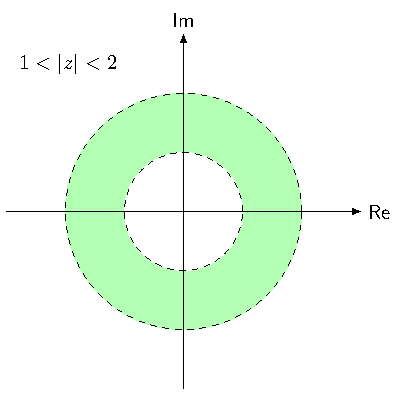
\includegraphics[scale=0.75]{annulus}\quad 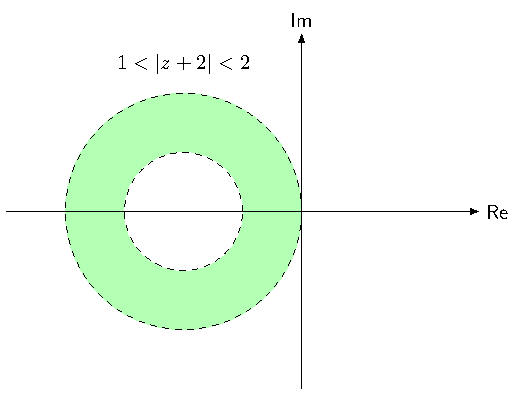
\includegraphics[scale=0.75]{annulus2}
\end{center}

\item[(c)] Write $z=x+iy$, then $z-i = x+i(y-1)$ and so
\begin{align*}
\set{z\in \C: 1 < \Im(z-i) <2 } &= \set{ x+iy \in \C : 1<y-1 <2 } \\
&= \set{x+iy \in \C: 2<y<3},
\end{align*}
which is the infinite horizontal band bounded by the lines $y=2$ and $y=3$.
\begin{center}
\oldincludegraphics[scale=0.75]{band}
\end{center}
\end{enumerate}
\end{answer}
\question 
\begin{parts}
\part Prove that for two nonzero complex numbers $z_1$ and $z_2$ we have
\[
\abs{z_1z_2} = \abs{z_1} \cdot \abs{z_2} \quad\text{ and }\quad \arg(z_1z_2)=\arg(z_1)\arg(z_2)
\]
(hint: write $z_1$ and $z_2$ in polar form).  Is it always true that $\Arg(z_1z_2)=\Arg(z_2)+\Arg(z_2)$?
\begin{answer}
Writing
\[
z_1=\polar{r_1}{\theta_1}\quad\text{and}\quad z_2=\polar{r_2}{\theta_2}
\]
we see that
\begin{align*}
z_1z_2&=r_1r_2 \left( \cos(\theta_1)\cos(\theta_2)-\sin(\theta_1)\sin(\theta_2) +i \left[ \cos(\theta_1)\sin(\theta_2)+\cos(\theta_2)\sin(\theta_1) \right] \right) \\
& = r_1r_2 \left( \cos(\theta_1+\theta_2)+i \sin(\theta_1+\theta_2) \right).
\end{align*}
Thus
\[
\abs{z_1z_2}=r_1r_2=\abs{z_1}\cdot \abs{z_2}\quad\text{and}\quad \arg(z_1z_2)=\theta_1+\theta_2=\arg(z_1)+\arg(z_2).
\]
It is not always true that $\Arg(z_1z_2)=\Arg(z_1)+\Arg(z_2)$.  Indeed, if $z_1=z_2=-1$ we have $\Arg (-1)=\pi$ but
\[
\Arg ((-1)(-1)) = \Arg (1) = 0.
\]
\end{answer}
\part Show that $\exp(z_1)\exp(z_2) = \exp(z_1+z_2)$.
\begin{answer}
With $z_1=x_1+iy_1$ and $z_2=x_2+iy_2$ a similar calculation to part (a) shows that
\begin{align*}
\exp(z_1)\exp(z_2) &= \polar{e^{x_1}}{y_1} \polar{e^{x_2}}{y_2} \\
 & = \polar{e^{x_1}e^{x_2}}{y_1+y_2} \\
 & = \polar{e^{x_1+x_2}}{y_1+y_2} = \exp(z_1+z_2).
\end{align*}
\end{answer}
\end{parts}
\question Write down the $3^{rd}$ roots of $-8$ in Cartesian form.
\begin{answer}
Writing $-8=\polar{8}{\pi}$, the three cubic roots are of the form $\polar{\sqrt[3]{8}}{(\pi+2k\pi)/3}$ for $k=0,1,2$.  In polar form, these are
\[
\polar{2}{\pi/3}, \quad \polar{2}{\pi} \quad\text{and}\quad\polar{2}{5\pi/3},
\]
or in Cartesian form $1+\sqrt{3},\ -2$ and $1-\sqrt{3}$ respectively.

\end{answer}

\question Find the values of $z$ for which $z^2+4iz-1=0$.  Which of these values lies inside the circle $C=\set{z \in \C: \abs{z}=1}$.
\begin{answer}
This is simply the usual quadratic formula: the roots of this polynomial are given by
\[
\frac{-4i\pm \sqrt{(4i)^2-4(1)(-1)}}{2} = \frac{-4i\pm i \sqrt{12}}{2} = i (-2 \pm  \sqrt{3}).
\]
To see which of these lies inside the circle $\abs{z}=1$, we examine the modulus and see that $\abs{i(-2 + \sqrt{3})} \approx 0.071<1$ and $\abs{i(-2-\sqrt{3})} \approx 1.93>1$. Thus only $i(-2+\sqrt{3})$ lies inside this circle.
\end{answer}


\question Show that $\Re (z) \leq \abs{ \Re (z)} \leq \abs{z}$ and $\abs{\Re (z)}+\abs{\Im (z)} \leq \sqrt{2} \abs{z}$.
\begin{answer}
The fact that $\Re (z) \leq \abs{ \Re (z)}$ is trivial.  Moreover,  writing $z=x+iy$ we see that
\[
\abs{\Re(z)} = \sqrt{x^2} \leq \sqrt{x^2+y^2}
\]
since $x^2 \leq x^2+y^2$ (and the square root function is increasing).

For the second inequality, note that with $z=x+iy$,
\begin{align*}
\left( \abs{\Re (z)}+\abs{\Im (z)} \right)^2 & = \left( \abs{x}+\abs{y} \right)^2 \\
& \leq \left( \abs{x}+\abs{y} \right)^2  + \overbrace{\left( \abs{x}-\abs{y} \right)^2}^{\geq 0}  \\
& = x^2+y^2+2\abs{xy} + x^2 + y^2 - 2\abs{xy} \\
& = 2(x^2+y^2) = 2 \abs{z}^2.
\end{align*}
Taking square roots of both sides yields the required inequality.
\end{answer}
\end{questions}

\setcounter{page}{1}
% !TEX root = exercises.tex

\exercisetitle{Exercise Sheet 1}

\begin{questions}
\question Use the triangle inequality $\abs{z_1-z_2} \leq \abs{z_1} + \abs{z_2}$ to prove the reverse triangle inequality:
\[
\abs{z_1-z_2} \geq \abs{\abs{z_1}-\abs{z_2}}
\]
\begin{answer}
The triangle inequality gives
\begin{align*}
\abs{z_1} & = \abs{z_1-z_2+z_2} \leq \abs{z_1-z_2} + \abs{z_2}  \\
\abs{z_2} & = \abs{z_2-z_1+z_1} \leq \abs{z_2-z_1} + \abs{z_1}\ (=\abs{z_1-z_2}+\abs{z_1}).
\end{align*}
Rearranging gives the two inequalities
\begin{align*}
\abs{z_1-z_2} & \geq \abs{z_1} - \abs{z_2} \\
\abs{z_1-z_2} & \geq \abs{z_2} - \abs{z_1},
\end{align*}
or in other words
\[
\abs{z_1-z_2} \geq \max \left( \abs{z_1}-\abs{z_2} , \abs{z_2} - \abs{z_1} \right) = \abs{\abs{z_1} - \abs{z_2} }.
\]
\end{answer}
\question Use the triangle and reverse triangle inequalities to show that for all $z$ on the circle $\abs{z}=2$, we have
\[
\abs{z+2} \leq 4 \text{ and } \abs{z-3+4i} \geq 3.
\]
Describe these inequalities geometrically.
\begin{answer}
If $\abs{z}=2$ then the triangle inequality ensures that
\[
\abs{z+2} \leq \abs{z}+2 = 4,
\]
and the backwards triangle inequality gives
\begin{align*}
\abs{z-3+4i} & = \abs{z-(3-4i)} \\
& \geq \abs{ \abs{z} - \abs{3-4i} } \\
& = \abs{2-5} = 3.
\end{align*}
Geometrically, these inequalities show respectively that the circle $\abs{z}=2$ is
\begin{itemize}
\item Contained in the disc with centre $-2$ and radius $4$ (i.e., the disc $\abs{z+2} \leq 4$), and
\item Outside of the disc with centre $3-4i$ and radius $3$.
\end{itemize}
\begin{center}
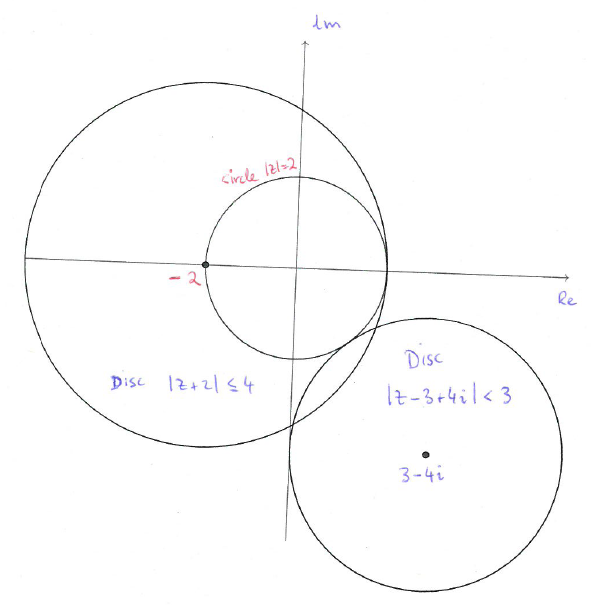
\includegraphics[scale=0.5]{ex1_q2}
\end{center}
\end{answer}
\question Use the triangle and reverse triangle inequalities to show that for all $z$ on the circle $\abs{z+3i}=3$ we have
\[
\abs{z-4} \leq 8,\quad \abs{z+5i}\geq 1 \text{ and } \abs{ \frac{z-4}{z+5i} } \leq 8.
\]
\begin{answer}

As with the previous question, the triangle inequality yields
\begin{align*}
\abs{z-4} & = \abs{z+3i-(3i+4)} \\
& \leq \abs{z+3i} + \abs{3i+4} \\
&=3+5=8.
\end{align*}
and the backwards triangle inequality yields
\begin{align*}
\abs{z+5i} & = \abs{z+3i+2i} \\
& \geq \abs{ \abs{z+3i} - \abs{2i} } \\
&=3-2=1.
\end{align*}
The third inequality is then obvious.
\end{answer}
\question Let $L$ be the line segment $[0,h]$ where $h \in \C$ and $\abs{h} < r$.  Show that if $\beta \in \C$ with $\abs{\beta}>2r$ and $z \in L$ then
\[
\abs{\frac{h-z}{\beta-z}} < \frac{\abs{h}}{r}.
\]
Do this using the reverse triangle inequality.  It can also be seen as follows.  Draw $L$ and two circles, both with centre $0$, $C_1$ with radius $r$ and $C_2$ with radius $2r$.  Why does $L$ lie inside $C_1$?  Where is $\beta$ on your diagram?  Why is $\abs{\beta-z}>r$?  If you can answer these three questions then the inequality should follow easily.
\begin{answer}

\begin{center}
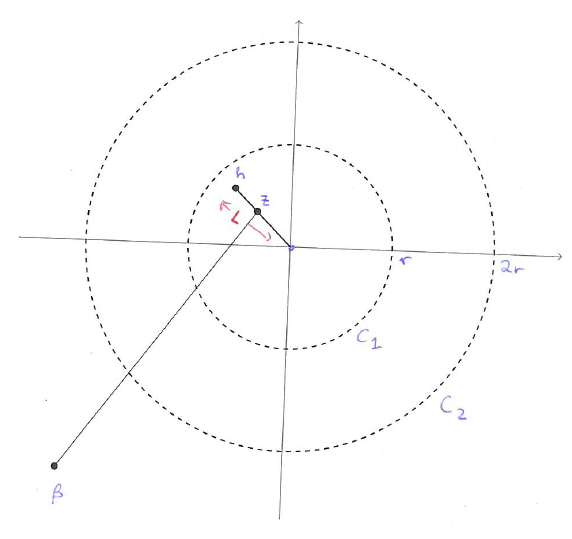
\includegraphics[scale=0.7]{ex1_q3}
\end{center}
Since $z$ lies on $L$, it is clear that $\abs{h-z} \leq \abs{h}$ (more formally, we can write $z=th$ for some $t$ with $0 \leq t \leq 1$, so that $\abs{h-z} = \abs{(1-t)h} = (1-t) \abs{h} \leq \abs{h}$).

The backwards triangle inequality, together with the fact that $\abs{z}<r<2r<\abs{\beta}$ gives
\begin{align*}
\abs{\beta - z} & \geq \abs{\abs{\beta}-\abs{z}} \\
& = \abs{\beta} - \abs{z} \\
&> 2r-r = r.
\end{align*}

Combining these two inequalities we see that
\begin{align*}
\abs{ \frac{h-z}{\beta - z} } &= \frac{\abs{h-z}}{\abs{\beta -z}} \\
 & \leq \frac{\abs{h}}{\abs{\beta - z}} \\
 & < \frac{\abs{h}}{r}.
\end{align*}

\end{answer}
\question The function $\mathbf{f}: \R^2 \to \R^2$ is defined by
$
\mathbf{f} (x,y)=(0,2y).
$
Show that the corresponding complex function $f:\C \to \C$ is
$
f(z) = z- \conj{z},
$
and that
\[
\lim_{h \to 0} \frac{f(z_0+h)-f(z_0)}{h}
\]
does not exist at any point $z_0 \in \C$.
\begin{answer}
The corresponding function is
\[
f(z) = f(x+iy) = i(2y) = i ( 2 \Im (z) ) = 2i \cdot \frac{z-\conj{z}}{2i} = z - \conj{z}.
\]
If $z_0 \in \C$ and $h \in \C \backslash \set{0}$ then
\[
\frac{f(z_0+h)-f(z_0)}{h} = \frac{(z_0+h)-\conj{(z_0+h)} - (z-\conj{z})}{h} = \frac{h-\conj{h}}{h} = 1- \frac{\conj{h}}{h}.
\]
Looking at restricted limits along the real and imaginary axes:
\[
1-\frac{\conj{h}}{h} \to \begin{cases}
1-1=0 & \text{ as } h \to 0, h \in \mathbb{R} \\
1-(-1)=2 & \text{ as } h \to 0, h \in i \R.
\end{cases}
\]
Since the restricted limits are not equal the (unrestricted) limit does not exist for any $z_0 \in \C$.

\end{answer}
\question Same as question 5 but with
\[
\mathbf{f}(x,y)=(x^2-y^2-x,2xy+y+1) \quad\text{ and }\quad f(z)=z^2-\conj{z}+i.
\]
\begin{answer}
This time, it is easier to start with the complex function $f$ and substitute $z=x+iy$:
\begin{align*}
f(z) & = z^2-\conj{z} + i \\
& = (x+iy)^2-(x-iy)+i \\
& = x^2-y^2+i2xy -x +iy +i \\
& = x^2-y^2-x + i \left( 2xy+y+1 \right),
\end{align*}
which shows that $f$ corresponds to the function $\mathbf{f}:\R^2 \to \R^2$ where
\[
\mathbf{f} (x,y) = \left( x^2-y^2-x, 2xy+y+1 \right).
\]
For $z_0 \in \C$ and $h \in \C \backslash \set{0}$ the difference quotient is
\begin{align*}
\frac{f(z_0+h)-f(z_0)}{h} & = \frac{(z_0+h)^2-\conj{(z_0+h)}+i-(z_0^2-\conj{z_0}+i )}{h} \\
& = h+2z_0-\frac{\conj{h}}{h}.
\end{align*}
Looking at some restricted limits:
\begin{align*}
\rlim{h \to 0}{h \in \R \backslash \set{0}} \frac{f(z_0+h)-f(z_0)}{h} & = 2z_0-1 \\
\rlim{h \to 0}{h \in i\R \backslash \set{0}} \frac{f(z_0+h)-f(z_0)}{h} & = 2z_0+1. \\
\end{align*}
These are not equal for any $z_0 \in \C$, so the unrestricted limit
\[
\lim_{h \to 0} \frac{f(z_0+h)-f(z_0)}{h}
\]
does not exist at any $z_0 \in \C$. 
\end{answer}
\question Let $f:\C \to \C$ be defined by $f(z) = \abs{z}^2$.  Show that $f$ is differentiable at $z=0$ and nowhere else.
\begin{answer}
Since $\abs{z}^2 = z \conj{z}$,
\begin{align*}
\frac{f(z_0+h)-f(z_0)}{h} &= \frac{(z_0+h)\conj{(z_0+h)}-z_0\conj{z_0}}{h} \\
& = \frac{z_0\conj{h}+h\conj{z_0}+h\conj{h}}{h} \\
&= z_0\frac{\conj{h}}{h} + \conj{z_0}+\conj{h} \\
& \longrightarrow
\begin{cases}
2z_0 & \text{ as }h \to 0,\ h \in \R \backslash \set{0} \\
0 & \text{ as } h \to 0, h \in i\R \backslash \set{0}.
\end{cases}
\end{align*}
For $z_0 \neq 0$, the restricted limits are not equal, hence the unrestricted limit does not exist and so $f$ is not differentiable at any point $z_0 \in \C \backslash \set{0}$.

At $z_0=0$, we have
\[
\lim_{h \to 0} \frac{f(0+h)-f(0)}{h} = \lim_{h \to 0} \conj{h} = 0,
\]
so that $f$ is differentiable at $0$ with $f'(0)=0$.
\end{answer}
\question Use the rules of differentiation to find the derivatives of the following functions:
\begin{parts}
\part $f(z) = \left( z^2+4 \right)^3$
\part $g(z) = \dfrac{z+i}{z-i}$.
\end{parts}
Find the values of $f'(i)$ and $g'(1)$.
\begin{answer}
\begin{parts}
\part Since $f$ is the composition of holomorphic functions, we can use the chain rule to find $f'(z)$:
\[
f'(z) = 3 ( z^2+4)^2(2z) = 6z(z^2+4)^2 \quad \text{ for all } z \in \C,
\]
and
\[
f'(i) = 6i (i^2+4)^2 = 6i(3)^2 = 54i.
\]
\part Since the functions $z \mapsto z\pm i$ are holomorphic on $\C$, $g$ is holomorphic on $\C \backslash \set{i}$, and the quotient rule gives
\[
g'(z) = \frac{(z-i)(1)-(z+i)(1)}{(z-i)^2} = \frac{-2i}{(z-i)^2}
\]
for all $z \in \C \backslash \set{i}$.  Hence
\[
g'(1) = \frac{-2i}{(1-i)^2} = \frac{-2i}{-2i} = 1.
\]
\end{parts}
\end{answer}

\end{questions}

\setcounter{page}{1}
% !TEX root = exercises.tex

\exercisetitle{Exercise Sheet 2}

\begin{questions}
\question For each function $f$ below, write $f$ in the form
\[
f(z) = f(x+iy) = u(x,y)+iv(x,y)
\]
and determine whether or not the Cauchy-Riemann equations are satisfied:
\[ (a)\ f(z) = \exp(i\ \conj{z})\quad  (b)\ f(z) = z + \dfrac{1}{z}\quad (c)\ f(z)=z^3.\]

In the cases where $f$ is differentiable, find the derivative of $f$ both using the rules of differentiation and using the Cauchy-Riemann equations.
\begin{answer}
\begin{parts}
\part We have 
\[
f(x+iy) = \exp (i (x-iy) ) = \exp (y+ix ) = \underbrace{e^{y} \cos (x) }_{u(x,y)} + i \underbrace{e^{y} \sin (x)}_{v(x,y)}.
\]
The corresponding partial derivatives are
\begin{align*}
\pd{u}{x} & = -e^{y} \sin(x) & \pd{v}{y} = e^{y} \sin(x) \\
\pd{u}{y} & = e^{y} \cos (x) &  \pd{v}{x} = e^{y} \cos (x).
\end{align*}
The Cauchy Riemann Equations are satisfied at a point $x+iy \in \C$ if and only if both
\[
e^y \sin(x) = -e^{y} \sin(x)\quad\text{and}\quad e^{y} \cos (x) = - e^{y} \cos (x).
\]
Since $e^y$ is never zero, this can only occur if $\sin(x)=\cos(x)=0$, which is impossible.  

\part For all $x +iy \in \C \backslash \set{0}$, 
\begin{align*}
f(x+iy) &= (x+iy) + \frac{1}{x+iy} \\
& = (x+iy) + \frac{x-iy}{x^2+y^2} \\
& = \underbrace{\left( x+ \frac{x}{x^2+y^2}  \right)}_{u(x,y)} + i \underbrace{\left( y-\frac{y}{x^2+y^2} \right) }_{v(x,y)}
\end{align*}
and the corresponding partial derivatives are
\begin{align*}
& \pd{u}{x} = 1+\frac{y^2-x^2}{(x^2+y^2)^2} && \pd{u}{y} = \frac{-2xy}{(x^2+y^2)^2} \\
& \pd{v}{x} = \frac{2xy}{(x^2+y^2)^2} && \pd{v}{y} = 1 - \frac{x^2-y^2}{(x^2+y^2)^2}.
\end{align*}
Hence the Cauchy Riemann equations are satisfied at every $x+iy \in \C \backslash \set{0}$.  Using the Cauchy Riemann equations to find the derivative of $f$, we get
\begin{align*}
f'(x+iy ) & = \pd{u}{x} + i \pd{v}{x} \\
& = \left( 1+\frac{y^2-x^2}{(x^2+y^2)^2} \right) + i \left( \frac{2xy}{(x^2+y^2)^2} \right) \\
& = 1 + \frac{y^2-x^2+i2xy}{(x^2+y^2)^2} \\
& = 1 - \frac{x^2-y^2-i2xy}{(x^2+y^2)^2} \\
& = 1 - \frac{(x-iy)^2}{\left[ (x+iy)(x-iy) \right]^2} \\
& = 1 - \frac{1}{(x+iy)^2} = 1- \frac{1}{z^2},
\end{align*}
which agrees with the derivative of $f$ obtained from the rules of differentiation.
\part This time
\[
u(x,y) = x^3-3xy^2 \quad\text{and}\quad v(x,y)=3x^2y-y^3
\]
hence for all $x+iy \in \C$
\[
\pd{u}{x} = 3x^2-3y^2=\pd{v}{y} \quad\text{and}\quad \pd{u}{y}=-6xy=-\pd{v}{x}.
\]
Thus
\[
f'(x+iy) = \pd{u}{x} (x,y)+i\pd{v}{y}(x,y) = 3x^2-3y^2+i(6xy) = 3 \left( (x^2-y^2)+i(2xy) \right) = 3(x+iy)^2
\]
which agrees with the derivative obtained from the Chain Rule: $f'(z)=3z^2$.
\end{parts}
\end{answer}

\question Show that the Cauchy-Riemann equations are satisfied by the function $f$ defined on the open upper half plane $H_+=\set{ z \in \C: \Im (z) > 0 }$ by
\[
f(x+iy) = u(x,y)+iv(x,y) = \log \left( \sqrt{ x^2+y^2 } \right) + i \left( \frac{\pi}{2} - \arctan \left( \frac{x}{y} \right) \right).
\]
Assuming that $f$ is indeed holomorphic on $H_+$, show that
\[
f'(x+iy) = \frac{1}{x+iy}\quad \text{i.e., that }\quad f'(z) = \frac{1}{z}.
\]
\begin{answer}
We have
\begin{align*}
\pd{u}{x} &= \log' \left( \sqrt{ x^2+y^2 } \right) \cdot \pd{}{x} \left[ \sqrt{x^2+y^2} \right] \\
& = \frac{1}{\sqrt{x^2+y^2}} \cdot \frac{1}{2} (x^2+y^2)^{-\frac{1}{2}}(2x) \\
&=  \frac{x}{x^2+y^2}
\shortintertext{ and similarly }
\pd{u}{y} & = \frac{y}{x^2+y^2}.\\
\intertext{For the partial derivatives of $v$, we have}
\pd{v}{x} & = - \arctan ' \left( \frac{x}{y} \right) \cdot \pd{}{x} \left[ \frac{x}{y} \right] \\
& = \frac{-1}{(1+(\frac{x}{y})^2)} \cdot \frac{1}{y} \\
& = \frac{-1}{y+\frac{x^2}{y}} = \frac{-y}{x^2+y^2} \\
\shortintertext{and }
\pd{v}{y} & = - \arctan ' \left( \frac{x}{y} \right) \cdot \pd{}{y} \left[ \frac{x}{y} \right] \\
& = \frac{-1}{(1+(\frac{x}{y})^2} \cdot \frac{-x}{y^2} \\
& = \frac{x}{x^2+y^2}.
\end{align*}
Thus the Cauchy-Riemann equations 
\[
\pd{u}{x} = \pd{v}{y},\quad \pd{u}{y} = - \pd{v}{x}
\]
are satisfied everywhere in $H_+$.  Assuming moreover that $f$ is holomorphic on $H_+$, the derivative of $f$ is thus
\begin{align*}
f'(x+iy) & = \pd{u}{x} + i \pd{v}{x} \\
& = \frac{x}{x^2+y^2}+i \frac{-y}{x^2+y^2} \\
& = \frac{x-iy}{(x+iy)(x-iy)} = \frac{1}{x+iy}
\end{align*}
for all $x+iy \in H_+$ as required.
\end{answer}

\question Describe the geometric effect of applying the functions:
\begin{parts}
\part $f(z) = \dfrac{1}{z}$ to a small disc centred at $1-i$, and 
\part $g(z) = \exp(2iz)$ to a small disc centred at $\frac{\pi}{4}+i$.
\end{parts}
\begin{answer}
For a function $f$ that is holomorphic at a point $z_0$, we know that a small disc centred at $z_0$ is approximately mapped to a small disc centred at $f(z_0)$, and is scaled by a factor of $\abs{f'(z_0)}$ and rotated by an angle of $\arg (f'(z_0))$ about the point $f(z_0)$.
\begin{parts}
\part In this example, $f(1-i)=\dfrac{1}{1-i}=\dfrac{1}{2}+\dfrac{i}{2}$, so a small disc centred at $1-i$ is approximately mapped to a small disc centred at $\dfrac{1}{2}+\dfrac{i}{2}$.  Since $f'(z) = -\dfrac{1}{z^2}$ for all $z \in \C \backslash \set{0}$, we have $f'(i)=-\dfrac{1}{(1-i)^2} = \frac{i}{2}$.  Thus the disc is scaled by a factor of $\frac{1}{2}$ and rotated by an angle of $\frac{\pi}{2}$ about $\dfrac{1}{2}-\dfrac{i}{2}$.
\part Mapped to a disc centred at $g(\frac{\pi}{4}+i)=e^{-2}i$, scaled by a factor of $2e^{-2}$ and rotated by an angle of $\pi$ about this point (clockwise or anticlockwise; it doesn't matter this time).
\end{parts}
\end{answer}
\question  The \emph{set} of points $L=[0,1-2i]$ is a line segment.  It is also a \emph{path} because we have a parametrisation given by  $\gamma:[0,1] \to \C,\ \gamma(t) = (1-2i)t.$  Use this parametrisation to evaluate the integral
\[
\int_L \left( \Im (z) + 3i \right)\ dz.
\]
\begin{answer}

We have
\begin{align*}
\int_{\Gamma} ( \Im (z) + 3i )\ dz & = \int_0^1 \left( \Im ( \gamma (t) ) +3i \right) \gamma' (t)\ dt \\
& = \int_0^1 \left( -2t + 3i \right) (1-2i)\ dt \\
& = (1-2i) \int_0^1 (-2t +3i)\ dt \\
& = (1-2i) \left[ - t^2 +3it \right]_0^1 \\
& = (1-2i)(-1+3i) = 5 + 5i.
\end{align*}

\end{answer}
\question Find the value of
\[
\int_{\Gamma_1} f(z)\ dz \text{ and } \int_{\Gamma_2} f(z)\ dz,
\]
where $f(z) = 3 \conj{z}$, $\Gamma_1$ is the straight line path from $0$ to $-i$ and $\Gamma_2$ is the straight line path from $1-i$ to $1+i$.
\begin{answer}
For the path $\Gamma_1$ we use the parametrisation $\gamma_1:[0,1] \to \C$, $\gamma_1 (t) = -it.$  Then $\gamma_1'(t)=-i$ and $f(\gamma_1(t)) = 3it$.  Hence
\[
\int_{\Gamma_1} f = \int_0^1 (3it)(-i)dt = \int_0^1 3t\ dt = \frac{3}{2}.
\]
Parametrise $\Gamma_2$ with $\gamma_2:[0,1] \to \C$, where
\[
\gamma_2 (t) = (1-i) + t \left[ 1+i-(1-i) \right] = 1+i(2t-1).
\]
We get
\[
\int_{\Gamma_2} f = 6i.
\]
\end{answer}





\question Fix a point $z_0 \in \C$ and define a complex function $f$ via
\[
f(z) = (z-z_0)^n
\]
where $n \in \mathbb{Z}$.  Find the value of
\[
\int_{\Gamma} f(z)\ dz,
\]
where $\Gamma$ is the circle with centre $z_0$ and radius $r>0$, traversed in the anticlockwise direction (use the parametrisation $\gamma:[0,2\pi] \to \C, \ \gamma (t) = z_0 + r \left( \cos (t) + i \sin (t) \right)$).  Do this separately for the cases $n=-1$ and $n \neq -1$.

(Hint: for the case $n \neq -1$, you need to show that
\[
\frac{d}{dt} \left[ \left( \cos(t)+i \sin(t) \right)^{n+1} \right] = i(n+1) \left( \cos(t)+i \sin(t) \right)^{n+1}
\]
and then use the (real) Fundamental Theorem of Calculus).
\begin{answer}
Following the hint, we first note that
\begin{align*}
\frac{d}{dt} \left[ \left( \cos(t)+i \sin(t) \right)^{n+1} \right] & = (n+1) \left( \cos(t)+i \sin(t) \right)^{n} \left( - \sin (t)+i \cos(t) \right) \\
& = (n+1) \left( \cos(t)+i \sin(t) \right)^{n} i \left( \cos(t)+i \sin(t) \right) \\
& = i(n+1) \left( \cos(t)+i \sin(t) \right)^{n+1}.
\end{align*}
We have
\[
f(\gamma(t))=\left( \gamma(t)-z_0 \right)^n = r^n \left( \cos (t)+i \sin (t) \right)^n,\quad \gamma'(t) = i r\left( \cos(t) + i \sin (t) \right).
\]
Hence for $n \neq -1$,
\begin{align*}
\int_{\Gamma} (z-z_0)^n & = \int_0^{2\pi} i r^{n+1} \left( \cos(t) + i \sin (t) \right)^{n+1}\ dt &&\\
& = \frac{r^{n+1}}{n+1} \int_0^{2\pi} \frac{d}{dt} \left[ \left( \cos(t) + i \sin (t) \right)^{n+1} \right]\ dt && \\
& = \frac{r^{n+1}}{n+1} \left[ \left( \cos(t) + i \sin (t) \right)^{n+1} \right]_0^{2\pi} && \text{ by FTC }\\
& = \frac{r^{n+1}}{n+1} \left[ 1+0i-(1+0i) \right] = 0 &&.
\end{align*}
If $n=-1$ then
\[
\int_{\Gamma} (z- z_0)^{-1} = \int_0^{2\pi} \frac{1}{r(\cos(t)+i\sin(t) )} \cdot ir (\cos(t)+i\sin(t) )\ dt =  \int_0^{2\pi} i\ dt = i2\pi.
\]


\end{answer}
\question Let $f,g:U \to \C$ be continuous, and let $\Gamma$ be a smooth path contained in $U$ parametrised by $\gamma:[a,b] \to \C$.  Prove that
\begin{parts}
\part for every constant $\alpha \in \C$ we have $\displaystyle \int_{\Gamma} ( f + \alpha g ) = \int_{\Gamma} f + \alpha \int_{\Gamma} g$, and
\part if $\tilde{\Gamma}$ denotes the reverse of $\Gamma$, we have $\displaystyle \int_{\tilde{\Gamma}} f = - \int_{\Gamma} f$.  As a hint, parametrise $\tilde{\Gamma}$ using $\tilde{\gamma}:[a,b] \to \C$, $\tilde{\gamma}(t)=(a+b-t)$, and use the substitution $s=a+b-t$.
\end{parts}
\begin{answer}
\begin{parts}
\part 
\begin{align*}
\int_{\Gamma} ( f + \alpha g ) & = \int_a^b (f + \alpha g )(\gamma(t)) \gamma'(t)\ dt \\
& = \int_a^b \left( f(\gamma(t)) + \alpha g(\gamma(t)) \right) \gamma' (t)\ dt \\
& = \int_a^b \left( f(\gamma(t)) \gamma'(t) + \alpha g (\gamma(t))\gamma'(t) \right)\ dt 
\end{align*}
Then using linearity of the real integral this becomes
\[
\int_a^b f(\gamma(t)) \gamma'(t)\ dt + \alpha \int_a^b g (\gamma(t))\gamma'(t)\ dt = \int_{\Gamma} f + \alpha \int_{\Gamma} g.
\]
\part Following the hint,
\begin{align*}
\int_{\tilde{\Gamma}} f & = \int_a^b f ( \tilde{\gamma} (t) ) \tilde{\gamma}' (t)\ dt \\
& = \int_a^b f ( \gamma(a+b-t) ) \left( - \gamma '(a+b-t) \right)\ dt
\end{align*}
and using the substitution $s=a+b-t$, we have $ds=-dt$ and the limits are reversed, so the above becomes
\begin{align*}
\int_b^a f ( \gamma (s) ) \left( - \gamma'(s) \right) (- ds) & = \int_b^a f (\gamma(s))\gamma'(s)\ ds \\ 
& = - \int_a^b f(\gamma(s)) \gamma'(s)\ ds \\
& = - \int_{\Gamma} f.
\end{align*}
\end{parts}
\end{answer}
\end{questions}
\setcounter{page}{1}
% !TEX root = exercises.tex

\exercisetitle{Exercise Sheet 3}

\begin{questions}
\question Find antiderivatives for the following functions:
\begin{parts}
\part $f(z) = \alpha + \beta(z-z_0)$,
\part $f(z) = (z-z_0)^n$,
\end{parts}
where $\alpha,\beta$ and $z_0 \in \C$ are constants and $n$ is an integer, $n \neq -1$.  Does $g(z)=(z-z_0)^{-1}$ have an antiderivative on $\C \backslash \set{z_0}$?  Question 6 on Exercise Sheet 2 may help here.  
\begin{answer}
\begin{enumerate}
\item[(a)] An antiderivative for $f$ on $\C$ is given by $F:\C \to \C$ where
\[
F(z) = \alpha z + \frac{1}{2} \beta z^2 - \beta z_0 z,
\]
since
\[
F'(z) = \alpha + ( \frac{1}{2} \beta ) (2z) - \beta z_0 = \alpha + \beta(z-z_0) = f(z)
\]
for all $z \in \C$.
\item[(b)] For $n \geq 0$ (respectively $n<-1$), and antiderivative for $f$ on $\C$ (respectively $\C \backslash \set{z_0}$) is given by $F$ where
\[
F(z) = \frac{1}{n+1} (z-z_0)^{n+1}.
\]
\end{enumerate}
The function $g$ does not have an antiderivative on $\C \backslash \set{0}$, since if it did, the Fundamental Theorem of Calculus would imply that
\[
\int_{\Gamma} g = 0
\]
where $\Gamma$ is the anticlockwise circular contour with centre $0$ and radius $1$.  We know from Exercise Sheet 2 that this integral has the value $2\pi i \neq 0$.
\end{answer}
\question Evaluate the following contour integrals:
\[
\int_{\mathcal{C}} z^3 \quad \text{ and } \quad \int_{\mathcal{C}} \frac{1}{z^2}
\]
along $\mathcal{C}$ where $\mathcal{C}$ is
\begin{parts}
\part any contour from $i$ to $-2$, and
\part any closed contour.
\end{parts}
For the second integral, you may assume that $\mathcal{C}$ does not contain $0$.
\begin{answer}
An antiderivative for $f(z) = z^3$ on $\C$ is given by the function $F$ with $F(z) = \frac{1}{4} z^4$.  Hence by the Fundamental Theorem of Calculus we have
\[
\int_{\mathcal{C}} z^3 = F(-2) - F(i) = \frac{1}{4} (-2)^4-\frac{1}{4} (i)^4 = \frac{15}{4}
\]
where $\mathcal{C}$ is any contour from $i$ to $-2$, and 
\[
\int_{\mathcal{C}} z^3 = 0
\]
when $\mathcal{C}$ is any closed contour.

Similarly $G(z) = \frac{-1}{z}$ is an antiderivative for $g(z) = \frac{1}{z}$ on $\C \backslash \set{0}$, and $\C \backslash \set{0}$ is a region in $\C$ (it is open and connected).  Hence by the Fundamental Theorem of Calculus we have
\[
\int_{\mathcal{C}} \frac{1}{z} = G(-2)-G(i) = \frac{-1}{-2} - \frac{-1}{i} = \frac{1}{2} -i
\]
for any contour $\mathcal{C}$ in $\C \backslash \set{0}$ from $i$ to $-2$, and
\[
\int_{\mathcal{C}} \frac{1}{z} =0
\]
for any closed contour $\mathcal{C}$ in $\C \backslash \set{0}$.

\end{answer}
\question Let $U$ be a region in $\C$ and let $f:U \to \C$ be holomorphic on $U$ with $f(z)$ real-valued for all $z \in U$.  Prove that $f$ is constant.
\begin{answer}
Write $f$ in the form
\[
f(x+iy)=u(x,y)+iv(x,y)
\]
where $u$ and $v$ are real-valued functions of two real variables.
If $f(z)$ is real valued then $v(x,y)=0$ on $U$, hence $\dfrac{\partial v }{\partial x} = \dfrac{\partial v}{\partial y}=0$ on $U$.

Since $f$ is holomorphic, $u$ and $v$ satisfy the Cauchy-Riemann equations, it follows that $\dfrac{\partial u}{\partial x} = \dfrac{\partial u}{\partial y}=0$ on $U$, hence
\[
f' = \frac{\partial u}{\partial x} + i \frac{\partial v}{\partial x} = 0
\]
on $U$. 

Since $U$ is connected, this implies that $f$ is constant by the Fundamental Theorem of Calculus.
\end{answer}


\question Find an upper estimate for
\[
\int_{\mathcal{C}} \frac{1}{1+z^4},
\]
where $\mathcal{C}$ is the upper semicircular contour from $R$ to $-R$ given by $\gamma:[0,\pi] \to \C$, $\gamma (t) = R \cos(t)+iR \sin (t)$.

\begin{answer}
We shall do this using the Estimation Lemma.  In order to apply the Lemma, we need to find $\ell{\Gamma}$ and an upper bound for $\abs{\frac{1}{1+z^4}}$ along $\mathcal{C}$.  Now, we know that
\[
\gamma '(t) = -R \sin(t) +i R \cos(t)
\]
with modulus
\[
\abs{\gamma'(t)} = \sqrt{ (-R\sin(t))^2+(R\cos(t))^2} = \sqrt{R^2(\sin^2(t)+\cos^2(t))} = R
\]
for all $t \in [0,\pi]$.  Hence the length of $\mathcal{C}$ is given by
\[
\ell(\mathcal{C})=\int_0^{\pi} \abs{\gamma'(t)} dt = \int_0^{\pi} R \ dt =\pi R.
\] 

Moreover, if $z$ lies in $\mathcal{C}$ then $z=\gamma(t)$ for some $t \in [0,\pi]$, hence
\[
\abs{z} = \abs{\gamma(t)} = \sqrt{(R\cos(t))^2+(R\sin(t))^2} = R.
\]
Using the backwards triangle inequality, for all $z \in \mathcal{C}$ we have
\[
\abs{1+z^4} \geq \abs{1-\abs{-z^4}} = \abs{1-R^4} = R^4-1
\]
(since $R>1$), and so
\[
\abs{\frac{1}{1+z^4}} \leq \frac{1}{R^4-1}
\]
whenever $z \in \mathcal{C}$.  Thus the Estimation Lemma tells us that
\[
\abs{\int_{\mathcal{C}} \frac{1}{1+z^4}} \leq \frac{1}{R^4-1} \cdot (\pi R) = \frac{\pi R}{R^4-1},
\]
so that $\pi R/(R^4-1)$ is an upper estimate for the integral $\int_{\mathcal{C}} 1/(1+z^4)$.


\end{answer}


\question Show that for all points $z$ on the circle $\set{z: \abs{z}=5}$ we have
\[
\abs{z-7} \leq 12 \quad \text{and}\quad \abs{\conj{z}+8} \geq 3,
\]
and use this to find an upper estimate for the integral
\[
\int_S \frac{z-7}{(\conj{z}+8)^2}\ dz
\]
where $S$ is the same circle oriented anticlockwise.

\begin{answer}
The first two inequalities can be shown using the triangle and backwards triangle inequalities respectively.  Using these, we have 
\[
\abs{\frac{z-7}{(\conj{z}+8)^2}} = \frac{\abs{z-7}}{\abs{\conj{z}+8}^2} \leq \frac{12}{3^2} = \frac{4}{3}
\]
for all $z \in S$.  The length of $S$ is $10\pi$, and so by the Estimation Lemma, we get the upper estimate
\[
\abs{
\int_S \frac{z-7}{(\conj{z}+8)^2}\ dz
}
\leq \frac{4}{3} \cdot 10\pi = \frac{40\pi}{3}.
\]
\end{answer}

\question Let $S_a$ be the anticlockwise square contour with corners at $\pm a(1+i),\pm a(1-i)$ where $a>0$.  Show that if $z \in S_a$ then
\[
\frac{1}{\abs{z}} \leq \frac{1}{a} \]
and hence
\[ \abs{ \int_{S_a} \frac{1}{z} dz } \leq 8,
\]
for all $a>0$.

\begin{answer}
Note that this square lies in the region outside the circle $\set{z:\C: \abs{z}=a}$.
\begin{center}
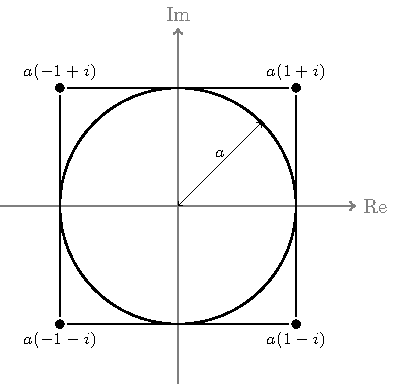
\includegraphics[scale=1]{squareandcircle}
\end{center}
Any point $z$ outside of this circle has modulus $\abs{z} \geq a$; in particular, this is true for any $z \in S_a$.  Hence for all such $z$, $\abs{\dfrac{1}{z}} \leq \dfrac{1}{a}$.

The length of each straight edge of $S_a$ is $2a$, and hence $\ell (S_a) = 8a$.  The Estimation Lemma then gives the required inequality.
\end{answer}

\question Prove each of the following:
\begin{parts}
\part For $z_0$ and $h$ in $\C$ we have $\displaystyle \int_{[z_0,z_0+h]} 1\ dz = h$.
\part For $f:U \to \C$ and $z_0 \in U$, $f(z_0) = \displaystyle \frac{1}{h} \int_{[z_1,z_1+h]} f(z_0)\ dz$.
\part If $\alpha$ is a complex number  and $M$ a fixed real number with $\abs{\alpha} \leq \epsilon M$ for all $\epsilon >0$ then $\alpha=0$.
\end{parts}
\begin{answer}
\begin{parts}
\part Using the parametrisation $\gamma:[0,1] \to \C$, $\gamma(t)=z_0+t(z_0+h-z_0) = z_0+th$, we have
$\gamma'(t)=h$ and $f(\gamma(t))=1$.  Hence
\[
\int_{[z_0,z_0+h]} 1dz = \int_0^1 f(\gamma(t)) \gamma '(t)\ dt = \int_0^1 1 (h) \ dt = h.
\]
Alternatively, using the antiderivative $F(z)=z$ for $f$, we have (by the Fundamental Theorem of Calculus)
\[
\int_{[z_0,z_0+h]} 1dz = F(z_0+h)-F(z_0)=z_0+h-z_0=h.
\]
\part Since $f(z_0)$ is a constant we have
\[
\frac{1}{h} \int_{[z_1,z_1+h]} f(z_0) dz = \frac{1}{h} f(z_0) \int_{[z_1,z_1+h]} 1 dz = \frac{1}{h} f(z_0) h = f(z_0)
\]
by the previous part.
\part Suppose that $\alpha \neq 0$.  Then $\abs{\alpha}>0$ (since for $z \in \C$ we have $\abs{z}=0$ if and only if $z=0$).  Setting $\epsilon = \abs{\alpha}/2M$ we have $\epsilon >0$, which implies that
\[
\abs{\alpha} \leq \epsilon M =  \frac{\abs{\alpha}}{2M} \cdot M = \frac{\abs{\alpha}}{2}.
\]
But this is only possible if $\abs{\alpha} =0$, a contradiction.  Hence $\abs{\alpha}=0$ and so $\alpha=0$.
\end{parts}
\end{answer}


\begin{comment}
\newpage


\question All of the proofs that have been done in lectures are examinable.  As some of these are quite long, you should be prepared to answer questions of the following format, where an outline of the proof is presented in the form of a series of statements.  For each numbered statement, provide a brief comment that explains or justifies it.  

\noindent{\bf Theorem (Cauchy's Theorem for a Triangle) } Let $\mathcal{R}$ be a simply connected region, $f$ a function that is holomorphic on $\mathcal{R}$ and let $T$ be a triangle in $\mathcal{R}$ with boundary $\partial T$.  Then
\[
\int_{\partial T} f =0.
\]
\medskip
{\bf Proof } 
There exists a nested sequence of triangles $\{ T_n \}$ such that
\[
\left( \frac{1}{4} \right)^n \left| \int_{\partial T} f \right| \leq \left| \int_{\partial T_n} f \right| \quad\text{ and }\quad \ell (\partial T_n ) = \left( \frac{1}{2} \right)^n \ell ( \partial T),
\]
and there is a point $z_0 \in \mathcal{R}$ with $z_0 \in T_n$ for all $n$.
\begin{enumerate}
\item[(1)] Given $\varepsilon >0$ there exists $\delta >0$ such that
\[
|z-z_0| < \delta \Longrightarrow \left| f(z)-f(z_0)-(z-z_0)f'(z_0) \right| \leq \varepsilon |z-z_0|
\]
\begin{answer}
Since $f$ is holomorphic on $\mathcal{R}$, $f$ is differentiable at $z_0$ and hence
\[
\lim_{z \to z_0} \frac{f(z)-f(z_0)}{z-z_0}
\]
exists and is equal to $f'(z_0)$.  

By the definition of a limit, given $\varepsilon>0$ there is $\delta >0$ such that
\begin{align*}
0< | z-z_0 | < \delta &\Rightarrow \left| \frac{f(z)-f(z_0)}{z-z_0}-f'(z_0) \right| < \varepsilon \\
& \Rightarrow \left| \frac{f(z)-f(z_0)-(z-z_0)f'(z_0)}{z-z_0} \right| < \varepsilon \\
& \Rightarrow \left| f(z)-f(z_0)-(z-z_0)f'(z_0) \right| < \varepsilon |z-z_0|.
\end{align*}
Finally, if $z=z_0$ then both sides of the final inequality are zero, which shows (1).
\end{answer}
\item[(2)] There exists $n$ such that $\ell ( \partial T_n) < \delta$ and $T_n \subset D(z_0;\delta)$.
\begin{answer}
Since $\ell ( \partial T)$ is fixed, we can choose $n$ large enough so that $\ell ( \partial T)/2^n < \delta$.  By the first (un-numbered) statement, for any such $n$ we have $\ell ( \partial T_n) < \delta$.

Since $z_0$ lies inside $T_n$, the distance from $z_0$ to any point on $\partial T_n$ is less than $\ell ( \partial T_n)$.
\end{answer}

\item[(3)]  For $z \in \partial T_n$
\[
\left| f(z)-f(z_0)-f'(z_0)(z-z_0) \right|< \epsilon \ell ( \partial T_n).
\]
\begin{answer}
By (2), for $z \in \partial T_n$ we have $|z-z_0| < \delta$, hence by (1), for all such $z$ we have
\[
\left| f(z)-f(z_0)-f'(z_0)(z-z_0) \right| \leq \varepsilon | z-z_0 | < \varepsilon \delta < \varepsilon \ell ( \partial T_n )
\]
the final inequality following from (2).
\end{answer}
\item[(4)] \hfil $\displaystyle \int_{\partial T_n} f(z)\ dz = \int_{\partial T_n} \left( f(z)-f(z_0)-f'(z_0)(z-z_0) \right)\ dz$\hfil
\begin{answer}
The (linear) function $z \mapsto f(z_0)+(z-z_0)f'(z_0)$ has an antiderivative on $\mathbb{C}$, and since $\partial T_n$ is a closed path,
\[
\int_{\partial T_n} f(z_0)+(z-z_0)f'(z_0)\ dz =0,
\]
so (4) follows from linearity of path integrals.
\end{answer}
\item[(5)]  \hfil $  \displaystyle \left| \int_{\partial T_n} f \right| \leq \varepsilon\ \left[\ell (\partial T_n ) \right]^2$ \hfil
\begin{answer}
The function $z \mapsto f(z) - f(z_0)-(z-z_0)f'(z_0)$ is bounded above on $\partial T_n$ by $ \varepsilon \ell ( \partial T_n )$ by (3), hence by the Estimation Lemma,
\[
\left| \int_{\partial T_n} f(z) - f(z_0)-(z-z_0)f'(z_0)\ dz \right| \leq \varepsilon \ell ( \partial T_n ) \cdot \ell ( \partial T_n ).
\]
Together with (4), this yields (5).
\end{answer}
\item[(6)] 
\hfil
$
 \displaystyle \left( \frac{1}{4} \right)^n \left| \int_{\partial T} f \right| \leq \left| \int_{\partial T_n} f \right| \leq \varepsilon\ \left[\ell (\partial T_n ) \right]^2 \leq \varepsilon \left(\frac{1}{4} \right)^n \left[ \ell ( \partial T) \right]^2.
$ \hfil
\begin{answer}
The first and last inequalities are given in the first (un-numbered) statement, the second was shown in (4).
\end{answer}
\item[(7)]\hfil $\displaystyle \int_{\partial T} f = 0 .$\hfil
\begin{answer}
By (6) we have
\[
\left| \int_{\partial T} f \right| \leq \varepsilon \left[ \ell ( \partial T ) \right]^2
\]
for all $\varepsilon >0$.  Since $\ell ( \partial T )$ is a constant, (7) follows.
\end{answer}
\end{enumerate}
\end{comment}



\end{questions}
\setcounter{page}{1}
% !TEX root = exercises.tex

\exercisetitle{Exercise Sheet 4}

\begin{questions}
\question Express each of the following complex numbers in Cartesian form $a+ib$:
\[
(a)\ \Log (i), \quad (b)\ \Log (ie)\quad (c)\  \Log (-1-i\sqrt{3}).
\]
\begin{answer}
Using $\Log (z) = \log \abs{z} + i \Arg (z)$,
\begin{align*}
\Log(i) & = \log \abs{i} + i \Arg (i) = \log(1)+i\frac{\pi}{2} = i\frac{\pi}{2}.\\
\Log (ie) &= \log(e)+i\frac{\pi}{2}  = 1 + i \frac{\pi}{2} \\
 \Log (-1-i\sqrt{3}) & =  \log (\sqrt{(-1)^2+(-\sqrt{3})^2}) + i \frac{-2\pi}{3}  = \log(2)-i \frac{2\pi}{3} 
\end{align*}
where $\log:[0,+\infty) \to \R$ denotes the real natural logarithm.
\end{answer}

\question Express each of the following complex numbers in Cartesian form $a+ib$:
\[
 (a)\ (1+i)^i, \quad (b)\ (ie)^{i\pi}, \quad (c)\ (-1-i\sqrt{3})^{1+i}.
\]
\begin{answer}
\begin{align*}
(1+i)^i & = \exp \left( i \Log (1+i) \right) = \exp \left( -\frac{\pi}{4} + i \frac{1}{2} \log(2) \right) \\
& = e^{-\frac{\pi}{4}} \cos ( \frac{1}{2} \log (2) ) + i e^{-\frac{\pi}{4}} \sin ( \frac{1}{2} \log (2) ). \\
(ie)^{i\pi} & = \exp \left( i \pi \Log (ie) \right) \\
& = \exp \left( i\pi - \frac{\pi^2}{2} \right) \\
& = e^{-\frac{\pi^2}{2}} \left( \cos(\pi)+i \sin (\pi) \right) \\
& = -e^{-\frac{\pi^2}{2}} \\
(-1-i \sqrt{3} )^{1+i} & = \exp \left( (1+i) \Log (-1-i \sqrt{3} ) \right) \\
& = \exp \left( (1+i) ( \log (2) - i \frac{2\pi}{3} ) \right) \\
& = \exp \left[ (\log(2)+\frac{2\pi}{3} )+i ( \log(2)- \frac{2\pi}{3}) \right] \\
& = \polar{e^{\log(2) + 2\pi/3}}{\log(2)-2\pi/3} \\
& = 2 \polar{e^{2\pi/3}}{\log(2)-2\pi/3} 
\end{align*}
\end{answer}
\question 
\begin{parts}
\part Use the definition $z^{\alpha} = \exp ( \alpha \Log (z) )$ to show that $z^3 =zzz$.
\part Show that $\Log(i^3) \neq 3 \Log (i)$
\part Define $\sqrt{z} = z^{1/2} ( = \exp ( \frac{1}{2} \Log (z) ) )$ for $z \in \C \backslash \set{0}$.  Where is the mistake in
\[
-1 = i^2 = ii = \sqrt{-1}\sqrt{-1} = \sqrt{-1 \times -1 } = \sqrt{1} =1?
\]
\part Show that for all $\alpha,\beta \in \C$ and $z \in \C \backslash \set{0}$ we have $z^{\alpha}z^{\beta} = z^{\alpha+\beta}$.  Is it true that $\Log(\alpha \beta) = \Log ( \alpha) + \Log ( \beta)$?
\end{parts}
\begin{answer}
\begin{parts}
\part Using the definition of the Principal $3^{rd}$ power function
\begin{align*}
z^3 & = \exp \left( 3 \Log (z) \right) \\
& = \exp \left( \Log(z)+\Log(z)+\Log(z) \right) \\
&= \exp \left(\Log(z) \right)\exp \left(\Log(z) \right)\exp \left(\Log(z) \right) \\
& = zzz.
\end{align*}
\part We have
\[
\Log (i^3) = \Log (-i) = - i\frac{\pi}{2}
\]
while
\[
3 \Log (i) = 3 \left( i \frac{\pi}{2} \right) = i \frac{3\pi}{2}.
\]
\part We do not have
\[
\sqrt{z} \sqrt{w} = \sqrt{zw}
\]
in general.  Indeed
\begin{align*}
\sqrt{-1}\sqrt{-1} & = \exp \left( \frac{1}{2} \Log(-1) \right) \exp \left( \frac{1}{2} \Log (-1) \right) \\
& = \exp ( \Log (-1) ) = -1
\end{align*}
while of course
\[
\sqrt{-1 \times -1 } = \sqrt{1} = \exp \left( \frac{1}{2} \Log (1) \right) = e^0=1.
\]
\part 
\[
z^{\alpha}z^{\beta} = \exp\left( \alpha \Log (z) \right) \exp \left( \beta \Log (z) \right) = \exp\left( (\alpha+\beta) \Log (z) \right) = z^{\alpha+\beta}.
\]
We do not have $\Log(\alpha\beta) = \Log(\alpha)+\Log(\beta)$ in general; for example if $\alpha=-1$ and $\beta=i$, then
\[
\Log(\alpha\beta) = \Log (-i) = -i \frac{\pi}{2}, \text{ while } \Log(\alpha)+\Log(\beta) = i\pi + i \frac{\pi}{2} = i \frac{3\pi}{2}.
\]
\end{parts}
\end{answer}
\question Recall that the Principal Logarithm function $\Log$ is holomorphic on the region $\C_{\pi}$, where \\ $\C_{\pi} = \set{z \in \C:z \neq 0 \text{ and } \Arg (z) \neq \pi }$. Let $F$ be the function defined by
\[
F(z) = \frac{1}{2i} \left( \Log (z+i)-\Log(z-i) \right).
\]
\begin{parts}
\part Describe (or sketch) the region $\mathcal{R}$ on which the function $F$ is holomorphic.
\part Show that $F$ is an antiderivative for the function $f:\mathcal{R} \to \C$ defined by
\[
f(z) = \frac{1}{z^2+1} \quad\text{for all}\quad z \in \mathcal{R}.
\]
\end{parts}
\begin{answer}
In general, for $z_0 = x_0+iy_0 \in \C$, the function
$
z \mapsto \Log (z-z_0)
$
is holomorphic on the region $\set{ z \in \C: z-z_0 \in \C_{\pi} }$.  For $z=x+iy \in \C$, $z-z_0$ is \emph{not} in $\C_{\pi}$ if and only if
\[
z-z_0 = (x-x_0) + i (y-y_0)
\]
lies on the negative real axis.  This occurs when
\begin{itemize}
\item $y-y_0=0$, i.e., when $y=y_0$, and
\item $x-x_0 \leq 0$, i.e. $x \leq x_0$.
\end{itemize}
Hence $z \mapsto \Log (z-z_0)$ is holomorphic on
\[
\C \backslash \set{z = x+iy \in \C: x \leq x_0 \text{ and } y=y_0},
\]
so in particular, $z \mapsto \Log (z+i)$ and $ z \mapsto \Log(z-i)$ are holomorphic on 
\[ \C \backslash \set{x+iy \in \C: x \leq 0 \text{ and } y=-1}\quad\text{ and}\quad \C \backslash \set{x:iy \in \C: x \leq 0 \text{ and } y=1} \]
respectively.

We know that our function $F$ is holomorphic on the region where both $z \mapsto \Log ( z+i)$ and $z \mapsto \Log (z-i)$ are holomorphic; i.e. the intersection of these two sets. This is the set
\[
 \C \backslash \set{ x+iy \in \C: x \leq 0 \text{ and } y= \pm 1 }.
\]

\end{answer}
\question Let $U$ be a starlit region with star centre $z_* \in U$ and  let $g:U \to \C$ be a holomorphic function.
\begin{parts}
\part Prove that if $g(z) \neq 0$ for all $ z \in U$, then the function $\dfrac{g'}{g}$ has an antiderivative on $U$, stating any results used (you may assume that $g$ holomorphic on $U$ implies $g'$ holomorphic on $U$).
\part Prove that if in addition $g(z) \in \C_{\pi}$ for all $z \in U$ then
\[
\int_{[z_*,z]} \frac{g'(\zeta)}{g(\zeta)}\ d\zeta = \Log (g(z)) + \alpha
\]
for some constant $\alpha$.
\end{parts}
\begin{answer}
Since $g$ is holomorphic and nonzero on $U$, $\dfrac{g'}{g}$ is also holomophic on $U$.

By The Existence of Antiderivatives on Starlit Regions, the function $G:U \to \mathbb{C}$ defined by
\[
G(z):= \int_{[z_*,z]} \frac{g'(\zeta)}{g(\zeta)}\ d\zeta
\]
is an antiderivative for $\dfrac{g'}{g}$ on $U$.

Since $\mathrm{Log}$ is holomorphic on $\mathbb{C}_{\pi}$ and $g(z) \in \mathbb{C}_{\pi}$ for all $z \in U$, $z \mapsto \mathrm{Log} (g(z))$ is holomorphic on $U$, with derivative
\[
\frac{d}{dz} \left[ \mathrm{Log} (g(z)) \right] = \frac{g'(z)}{g(z)}.
\]
Together with the first part this shows that
\[
\frac{d}{dz} \left[ \mathrm{Log} (g(z)) - G(z) \right] = 0
\]
on $U$. Since a starlit region is connected, the Fundamental Theorem of Calculus implies that
\[
z \mapsto \mathrm{Log} (g(z)) - G(z) 
\]
is constant.
\end{answer}

\question Evaluate the integral
\[
\int_{\mathcal{C}} \frac{\exp (2z)}{4z+i\pi}\ dz
\]
where $\mathcal{C}$ is (i) the anticlockwise contour whose points lie on the circle $\set{z:\abs{z}=1}$, and (ii) when $\mathcal{C}$ is the anticlockwise contour whose points lie on the circle $\set{z: \abs{z-2i}=2}$. The use of any Theorems made to obtain the value of these integrals should be justified.
\begin{answer}
$(i): \frac{\pi}{2},\quad (ii): 0 $.
\end{answer}
\question Evaluate the integral
\[
\int_{\mathcal{C}} \frac{\cos (z^2)}{3i+2z}\ dz,
\]
where (i) $\mathcal{C}$ is the anticlockwise contour whose points lie on the circle $\set{z:\abs{z}=1}$, and (ii) $\mathcal{C}$ is the anticlockwise contour whose points lie on the circle $\set{z: \abs{z}=5}$.  The use of any Theorems made to obtain the value of these integrals should be justified.
\begin{answer}
(i) The given function is holomorphic on $\C \backslash \set{ z: 3i+2z=0 }$, that is to say, on $\C \backslash \set{ -i \frac{3}{2}}$.  In particular, it is holomorphic on the simply connected region 
\[
\set{ z \in \C: \Im (z) > - \tfrac{5}{4} }
\]
which contains the (closed) contour $\mathcal{C}$.  Thus by Cauchy's Theorem for Starlit regions, 
\[
\int_{\mathcal{C}} \frac{\cos (z^2)}{3i+2z}\ dz=0.
\]

(ii) We have
\[
\frac{\cos(z^2)}{3i+2z} = \frac{g(z)}{z-z_0}
\]
where
\[
z_0 = -i \tfrac{3}{2} \quad \text{ and } \quad g(z) = \tfrac{1}{2} \cos (z^2).
\]
The function $g$ is holomorphic on $\C$ (which is simply connected), and $\mathcal{C}$ is a closed, simple anticlockwise contour that encloses $z_0$, so that by Cauchy's Integral Formula
\[
\int_{\mathcal{C}} \frac{\cos(z^2)}{3i+2z}\ dz = \int_{\mathcal{C}} \frac{g(z)}{z-(-i\frac{3}{2})}\ dz = 2\pi i g(-i \tfrac{3}{2}) = 2\pi i \tfrac{1}{2} \cos (- \tfrac{9}{4}) = i \pi \cos ( \tfrac{9}{4} ).
\]

\end{answer}

\question Evaluate the integral
\[
\int_{-\infty}^{+\infty} \frac{1}{x^2+6x+25}\ dx
\]
in the following way (compare Example 5.8 in the notes):
\begin{parts}
\part Define the complex function $f$ by
$
\displaystyle f(z) = \frac{1}{z^2+6z+25}$  and find $z_0$  and  $z_1$ so that $\displaystyle
f(z) = \frac{1}{(z-z_0)(z-z_1)}$ (where $z_0$ lies in the upper half-plane and $z_1$ in the lower half-plane). 
\begin{answer}
The roots of $z^2+6z+25$ can be found using the quadratic formula;
\begin{align*}
z & = \frac{-6 \pm \sqrt{6^2-4(25)(1)}}{2} \\
& = \frac{-6 \pm \sqrt{-64}}{2} \\
& = \frac{-6+i8}{2} = -3 \pm 4i.
\end{align*}
Hence
\[
f(z) = \frac{1}{(z-(-3+4i))(z-(-3-4i))}.
\]
\end{answer}
\part Choose a suitable function $g$, holomorphic on the simply connected region \\$\mathcal{R} = \set{z \in \C: \Im(z) > \frac{1}{2} \Im (z_1) }$, so that
\[
f(z) = \frac{g(z)}{(z-z_0)}.
\]
\begin{answer}
With $z_0=-3+4i$ and
\[
g(z) = \frac{1}{z-(-3-4i)}
\]
then
\[
f(z) = \frac{g(z)}{z-(-3+4i)}.
\]
Moreover, $g$ is holomorphic on $\C \backslash \set{ -3-4i}$, and in particular, on the simply connected region $\mathcal{R}:= \set{z \in \C: \Im (z) >-2 }$. 
\end{answer}
\part  Justify the use of Cauchy's Integral Formula to find
\[
\int_{\mathcal{C}_R} f = \int_{\mathcal{C}_R} \frac{g(z)}{(z-z_0)}\ dz,
\]
where $\mathcal{C}_R=L_R+S_R$ with $L_R$ the straight line path from $-R$ to $R$ and $S_R$ a suitable semicircular contour from $R$ to $-R$, with $R$  sufficiently large to apply the Theorem.
\begin{answer}
Once $R>5$, the contour simple closed anticlockwise contour $\mathcal{C}_R$ encloses $z_0$.  Moreover $\mathcal{C}_R$ is always contained in the simply connected region $\mathcal{R}$ of the previous part, and $g$ is holomorphic on this region.  Therefore, we may apply Cauchy's Integral formula:
\begin{align*}
\int_{\mathcal{C}_R} f = \int_{\mathcal{C}_R} \frac{g(z)}{z-(-3+4i)}\ dz & = 2\pi i g(-3+4i) \\
& = 2\pi i \cdot \frac{1}{(-3+4i)-(-3-4i)} \\
& = \frac{2\pi i}{8i} = \frac{\pi}{4},
\end{align*}
and this is valid for all $R>5$.
\end{answer}
\part Show that for large $R$ and $z \in S_R$, we have $\abs{z^2+6z+25} \geq R^2-6R-25$.
\begin{answer}
If $z \in S_R$ then $\abs{z}=R$, so that the reverse triangle inequality gives
\begin{align*}
\abs{z^2+6z+25} &\geq \abs{ \abs{z^2} - \abs{6z+25} }\\
& = \abs{\abs{z}^2-\abs{6z+25}} \\
& = \abs{ R^2-\abs{6z+25}}.
\end{align*}
By the triangle inequality,
\[
\abs{6z+25} \leq  6R + 25 \quad \text{ for all } z \in S_R.
\]
Moreover, if $R>10$, we have $25 < 2.5 R$ so that
\[
6R+25 < 6R+2.5 R < 10 R < R^2.
\]
Thus for $R>10$ and $z \in S_R$,
\[
\abs{z^2+6z+25} \geq R^2 - 6R - 25.
\]
\end{answer}
\part Use the Estimation Lemma to show that
\[
\abs{ \int_{S_R} f } \to 0 \text{ as } R \to \infty.
\]
\begin{answer}
By the previous part, for $R>10$ and $z \in S_R$ we have
\[
\abs{
\frac{1}{z^2+6z+25}
}
 \leq \frac{1}{R^2-6R-25}.
\]
Since the length of $S_R$ is $\pi R$, for all $R>10$ we have
\[
\abs{\int_{S_R} f} \leq \underbrace{\frac{1}{R^2-6R-25}}_{M} \cdot \underbrace{\pi R}_L = \frac{\pi}{R-6-\frac{25}{R}}
\]
by the Estimation Lemma.  Hence
\[
\abs{ \int_{S_R}} f \to 0 \quad \text{ as }\quad R \to \infty.
\]
\end{answer}
\part Deduce the value of
\[
\int_{-\infty}^{+\infty} \frac{1}{x^2+6x+25}\ dx.
\]
\begin{answer}
We have
\begin{align*}
\frac{\pi}{4} & = \int_{\mathcal{C}_R} f && \text{ for } R>5 \\
& = \lim_{R \to \infty} \left( \int_{C_R} f \right) && \\
&=  \lim_{R \to \infty} \left( \int_{L_R} f \right) + \lim_{R \to \infty} \left( \int_{S_R} f \right) && \\
& = \lim_{R \to \infty} \left( \int_{-R}^{R} \frac{1}{t^2+6t+25}\ dt \right) + 0 && \text{ by part (d) } \\
& = \int_{-\infty}^{\infty} \frac{1}{x^2+6x+25}\ dx. &&
\end{align*}

\end{answer}
\end{parts}

\question (Liouville's Theorem) Let $f:\C \to \C$ be holomorphic everywhere, and suppose that $f$ is bounded, i.e. there exists $M>0$ with $\abs{f(z)} \leq M$ for all $z \in \C$.  Show that $f$ is constant on $\C$, in the following way:
\begin{parts}
\part Let $z_1,z_2 \in \C$, and let $R>0$ be sufficiently large so that $z_1$ and $z_2$ are enclosed by the countour $\mathcal{C}_R$ consisting of the anticlockwise circle with centre $0$ and radius $R$. Use Cauchy's Integral Formula to write $f(z_1)-f(z_2)$ as a single integral along $\mathcal{C}_R$.
\begin{answer}
As $f$ is holomorphic on $\C$ and $\mathcal{C}_R$ is a simple, closed anticlockwise contour containing both $z_1$ and $z_2$, we can apply Cauchy's Integral formula (twice) to get
\[
\int_{\mathcal{C}_R} \frac{f(z)}{z-z_1}\ dz = 2 \pi i f(z_1) \quad \text{ and }\quad \int_{\mathcal{C}_R} \frac{f(z)}{z-z_2}\ dz = 2 \pi i f(z_2).
\]
Hence (since we may combine integrals along the same path)
\begin{align*}
f(z_1)-f(z_2) & = \frac{1}{2\pi i} \int_{\mathcal{C}_R} \frac{f(z)}{z-z_1}\ dz - \frac{1}{2\pi i} \int_{\mathcal{C}_R} \frac{f(z)}{z-z_2}\ dz \\
& = \frac{1}{2\pi i} \int_{\mathcal{C}_R} \left( \frac{f(z)}{z-z_1} - \frac{f(z)}{z-z_2} \right)\ dz \\
& = \frac{1}{2\pi i} \int_{\mathcal{C}_R} \frac{f(z)(z-z_2)-f(z)(z-z_1)}{(z-z_1)(z-z_2)}\ dz \\
& = \frac{1}{2\pi i} \int_{\mathcal{C}_R} \frac{f(z)(z_1-z_2)}{(z-z_1)(z-z_2)}\ dz.
\end{align*}
\end{answer}
\part Use the Estimation Lemma (and the backwards triangle inequality) to show that
\[
\abs{f(z_1)-f(z_2)} \leq M \frac{\abs{z_1-z_2}}{(R-\abs{z_1})(R-\abs{z_2})}\cdot 2\pi R
\]
for all (sufficiently large) $R$.
\begin{answer}
If $R> \max ( \abs{z_1}, \abs{z_2} )$ and $z \in \mathcal{C}_R$, then by the backwards triangle inequality
\[
\abs{z-z_1} \geq \abs{ \abs{z} - \abs{z_1}} = R - \abs{z_1}
\]
and similarly $\abs{z-z_2} \geq R - \abs{z_2}$.  Since $\abs{f(z)} \leq M$ we have
\begin{align*}
\abs{ \frac{f(z)(z_1-z_2)}{(z-z_1)(z-z_2)} }  &= \frac{\abs{f(z)} \cdot \abs{z_1-z_2}}{\abs{z-z_1} \cdot \abs{z-z_2}} \\
& \leq \frac{M \abs{z_1-z_2}}{(R-\abs{z_1})(R-\abs{z_2})}.
\end{align*}
The path $\mathcal{C}_R$ has length $2 \pi R$, thus by the Estimation Lemma
\[
\abs{ \int_{\mathcal{C}_R} \frac{f(z)(z_1-z_2)}{(z-z_1)(z-z_2)}\ dz } \leq M \frac{\abs{z_1-z_2}}{(R-\abs{z_1})(R-\abs{z_2})}\cdot 2\pi R
\]
\end{answer}
\part Deduce that $f(z_1)=f(z_2)$.
\begin{answer}
By parts (b) and (c) we have
\begin{align*}
\abs{f(z_1)-f(z_2)} &= \abs{ \frac{1}{2\pi i} \int_{\mathcal{C}_R} \frac{f(z)(z_1-z_2)}{(z-z_1)(z-z_2)}\ dz } \\
& \leq \abs{ \frac{1}{2\pi i} }  M \frac{\abs{z_1-z_2}}{(R-\abs{z_1})(R-\abs{z_2})}\cdot 2\pi R \\
& = \frac{MR \abs{z_1-z_2}}{(R-\abs{z_1})(R-\abs{z_2})} \\
& = \frac{M \abs{z_1-z_2}}{(1-\abs{z_1}/R)(R-\abs{z_2})}
\end{align*}
for all $R>\max(\abs{z_1},\abs{z_2})$.  Since $M$ and $\abs{z_1-z_2}$ are constants, it follows that
\[
\frac{M \abs{z_1-z_2}}{(1-\abs{z_1}/R)(R-\abs{z_2})} \to 0 \quad\text{as}\quad R \to \infty.
\]
Hence $\abs{f(z_1)-f(z_2)}=0$, or in other words $f(z_1)=f(z_2)$.
\end{answer}
\end{parts}
\end{questions}
\setcounter{page}{1}
% !TEX root = exercises.tex

\exercisetitle{Exercise Sheet 5}

\begin{questions}
\question Locate the poles of each of the following functions, and calculate the residues at these poles:
\begin{parts}
\part $f(z) = \dfrac{1}{z(i-z)^3}$
\part $f(z) = \dfrac{z^2}{(z^2+1)^2}$
\part $f(z) = \dfrac{\Log(z)}{(4z-i)^2}$
\part $f(z)=\dfrac{1}{\exp(z)-1}$.
\end{parts}
\begin{answer}
\begin{parts}
\part This time $f$ has a pole of order $1$ at $0$ and a pole of order $3$ at $i$.  With $g_1(z) = \frac{1}{(i-z)^3}$ and $h_1(z)=z$, the $g/h$ rule gives
\[
\Res (f;0) = \frac{g(0)}{h'(0)} = \frac{1}{(1) \cdot (i)^3}  = i.
\]
For the pole of order $3$ at $i$ we first rewrite
\[
f(z) = \frac{1}{z(-(z-i))^3} = - \frac{1}{z(z-i)^3}.
\]
Now, letting $g_2(z) = -z^{-1}$ we can use the formula
\[
\Res (f;i) = \frac{g_2''(i)}{2!}.
\]
We have $g_2'(z) = z^{-2}$ and $g_2''(z) = -2z^{-3}$, so that $g_2''(i)=-2/(i)^3 = -2i$ and hence
\[
\Res (f;i) = \frac{-2i}{2} = -i.
\]
\part Writing
\[
f(z) = \frac{z^2}{(z+i)^2(z-i)^2}
\]
we see that $f$ has poles of order $2$ at $z=\pm i$.  If $g_1 (z)=  \dfrac{z^2}{(z+i)^2}$ then
\[
g_1'(z) = \frac{(z+i)^2(2z)-2(z+i)z^2}{(z+i)^4},\quad g_1'(i) = \frac{(2i)^3-2(2i)i^2}{(2i)^4} = - \frac{i}{4}
\]
hence
\[
\Res (f; i) = \frac{g_1'(i)}{1!} = - \frac{i}{4}.
\]
Similarly, with $g_2(z) = \frac{z^2}{(z-i)^2}$,
\[
g_2'(z) = \frac{(z-i)^2(2z)-2(z-i)z^2}{(z-i)^4},\quad g_2'(-i) = \frac{(-2i)^2(2i)-2(-2i)(-2i)^2}{(-2i)^4} = \frac{i}{4}.
\]
Hence
\[
\Res (f;-i) = \frac{g_2'(i)}{1!} = \frac{i/4}{1} = \frac{i}{4}.
\]
\part Pole of order $2$ at $z=i/4$.  Write $f(z) = \dfrac{\Log(z)}{16 (z-\frac{i}{4})^2}$, then
\[
\Res(f;i/4) = \frac{1}{16} \cdot \frac{1}{(i/4)} = - \frac{i}{4}.
\]
\part Use the $g/h$ rule with $g(z)=1$ and $h(z)=\exp(z)-1$.  Then $h(z)=0$ whenever $\exp(z)=1$, i.e. at the points $z_k = 2\pi i k$ where $k \in \mathbb{Z}$, so $f$ has isolated singularities at these points.  Since $h'(z) = \exp(z),\ h'(z_k)=1$ for all $k$, and so each $z_k$ is a pole of order $1$ for the function $f$.  By the $g/h$ rule,
\[
\Res (f;z_k) = \frac{g(z_k)}{h'(z_k)} = 1.
\]
\end{parts}


\end{answer}
\question Evaluate
\[
\int_{\mathcal{C}} \frac{1}{z(z-1)(z+2)}\ dz,
\]
where $\mathcal{C}$ is the anticlockwise circle with centre $0$ and radius $3/2$.
\begin{answer}
The function $f$ defined by
\[
f(z) = \frac{1}{z(z-1)(z+2)}
\]
has isolated singularities at $0,1$ and $2$, and the first two of these are enclosed by $\mathcal{C}$.  The residues are
\begin{align*}
\Res (f;0) &= \frac{1}{(0-1)(0+2)}  = - \frac{1}{2} \\
 \Res (f;1) & = \frac{1}{1(1+2)}  = \frac{1}{3}.
\end{align*}
Hence by the Residue Theorem
\[
\int_{\mathcal{C}} \frac{1}{z(z-1)(z+2)}\ dz = 2\pi i \left( - \frac{1}{2} + \frac{1}{3} \right) = - \frac{i\pi}{3}.
\]
\end{answer}
\question Evaluate
\[
\int_{\mathcal{C}} \frac{1}{(z^2+1)^3}\ dz
\]
where $\mathcal{C}$ is the anticlockwise square with vertices $1,\ 1+2i, -1+2i$ and $-1$.
\begin{answer}
Using the factorisation $(z^2+1)^3=(z+i)^3(z-i)^3$, we see that this function, call it $f$, has poles of order $2$ at $z=\pm i$.  Of these, only the pole at $z=i$ is enclosed by $\mathcal{C}$, so that 
\[
\int_{\mathcal{C}} \frac{1}{(z^2+1)^3}\ dz = 2\pi i \Res (f;i).
\]
If we let $g(z) = \dfrac{1}{(z+i)^3}$ then
\[
f(z) = \frac{g(z)}{(z-i)^3},
\]
$g'(z) = -3 (z+i)^{-4}$ and $g''(z) = 12(z+i)^{-5}$.  Hence
\[
\Res (f;i) = \frac{g''(i)}{2!} = \frac{12}{2(2i)^5} = \frac{3}{16i}
\]
which gives
\[
\int_{\mathcal{C}} f = 2\pi i \left( \frac{3}{16i} \right) = \frac{3\pi}{8}.
\]
\end{answer}
\question Use contour integration to evaluate each of the following real integrals:
\begin{parts}
\part \hfil$\displaystyle
\int_0^{2\pi} \frac{1}{5+4 \sin \theta}\ d\theta 
$\hfil
\part \hfil$\displaystyle \int_0^{\infty} \frac{1}{x^4+1}\ dx$\hfil
\end{parts}
\begin{answer}
\begin{parts}
\part We use the fact that for a rational function $R$ of two (real) variables,
\[
\int_0^{2\pi} R( \cos(t), \sin (t) ) dt = \int_{\mathcal{C}} f
\]
where $\mathcal{C}$ is the anticlockwise unit circle and $f$ is the complex function defined by
\[
f(z) = R \left( [z+z^{-1}]/2 , [z-z^{-1}]/(2i) \right) \cdot \frac{1}{iz}.
\]
In this case, we have
\begin{align*}
f(z) & = \frac{1}{5+4[z-z^{-1}]/2i} \cdot \frac{1}{iz} \\
& = \frac{1}{2z^2+5iz-2} \\
& = \frac{1}{(2z+i)(z+2i)}.
\end{align*}
Then with $\mathcal{C}$ the anticlockwise unit circle, the only singularity of $f$ enclosed by $\mathcal{C}$ is at $z=-i/2$, and so
\begin{align*}
\int_0^{2\pi} \frac{1}{5+4 \sin \theta}\ d\theta &= \int_{\mathcal{C}} \frac{1}{(2z+i)(z+2i)}\ dz \\
& = 2\pi i \Res (f;-i/2) \\
& = 2\pi i \cdot \frac{1}{2(-i/2+2i)} = \frac{2\pi}{3}.
\end{align*}
\part 
We shall consider the complex function
\[
f(z) = \frac{1}{z^4+1}
\]
which is holomorphic everywhere in $\C$ except where $z^4=-1$; that is to say, $f$ is holomorphic on $\C \backslash \set{ e^{i\pi/4},\ e^{i3\pi/4},\ e^{i 5\pi/4},\ e^{i 7\pi/4} }$.  Let $\mathcal{C}_R = L_R+S_R$ where $R>1$, $L_R$ is the straight line path $[-R,R]$ and $S_R$ is the upper-semicircle with centre $0$ and radius $R$ from $R$ to $-R$ via $iR$; then the poles of $f$ enclosed by $\mathcal{C}_R$ are at $e^{i\pi/4}$ and $e^{i3\pi/4}$.

With $g(z)=1$ and $h(z)=z^4+1$, we have $h'(z)=4z^3$ so that by the $g/h$ rule,
\begin{align*}
\Res(f;e^{i\pi/4}) &= \frac{1}{4(e^{i\pi/4})^3} = \frac{1}{4e^{3\pi/4}} = \frac{1}{4(-a+ia)} \\
\Res(f;e^{i3\pi/4}) &= \frac{1}{4(e^{i3\pi/4})^3} = \frac{1}{4e^{9\pi/4}} = \frac{1}{4(a+ia)} \\
\end{align*}
where $a=1/\sqrt{2}$. So (for $R>1$) we have
\begin{align*}
\int_{\mathcal{C}_R} f &= 2\pi i \left( \text{ sum of residues at poles of $f$ inside $\mathcal{C}_R$} \right) \\
& = 2\pi i \left( \frac{1}{4(-a+ia)}+\frac{1}{4(a+ia)}) \right)
& = \frac{\pi}{\sqrt{2}}
\end{align*}
by the Residue Theorem.

We now show that 
\[
\lim_{R \to \infty} \int_{S_R} f =0
\]
using the Estimation Lemma.  Indeed, for $z \in S_R$, $\abs{z}=R$ and so by the reverse triangle inequality
\[
\abs{z^4+1} \geq \abs{ \abs{z^4} - \abs{1} } = \abs{ \abs{z}^4-1 } = R^4-1.
\]
Hence for all such $z$,
\[
\abs{ f(z) } = \abs{\frac{1}{z^4+1}} = \frac{1}{\abs{z^4+1}} \leq \frac{1}{R^4-1}.
\]
The Estimation Lemma then gives
\[
\abs{ \int_{S_R} f } \leq \frac{1}{R^4-1} \cdot \pi R = \frac{\pi R}{R^4-1}
\]
so that
\[
\int_{S_R} f \to 0 \quad\text{ as }\quad R \to \infty.
\]

Using the parametrisation $\gamma_L:[-R,R] \to \C$, $\gamma(t)=t$ of $L_R$, we have
\[
\int_{L_R} f = \int_{-R}^R \frac{1}{(t^4+1}\ dt.
\]
Hence
\begin{align*}
\frac{\pi}{\sqrt{2}} & = \int_{\mathcal{C}_R} f \\
& = \lim_{R \to \infty} \int_{\mathcal{C}_R} f \\
& = \lim_{R \to \infty} \int_{-R}^R \frac{1}{t^4+1}\ dt + \lim_{R \to \infty} \int_{S_R} f \\
& = \int_{-\infty}^{\infty} \frac{1}{t^4+1}\ dt.
\end{align*}
Since the integrand is even, it follows that
\[
\int_{0}^{\infty} \frac{1}{t^4+1}\ dt = \frac{1}{2} \int_{-\infty}^{\infty} \frac{1}{t^4+1}\ dt = \frac{\pi}{2\sqrt{2}}.
\]

\end{parts}
\end{answer}
\question Use contour integration to evaluate the following real integrals:
\begin{parts}
\part \[
\int_0^{2\pi} \frac{1}{16 \cos^2 (t)+25 \sin^2 (t)}\ dt.
\]
\begin{answer}
As before, we use the fact that for a rational function $R$ of two (real) variables,
\[
\int_0^{2\pi} R( \cos(t), \sin (t) ) dt = \int_{\mathcal{C}} f
\]
where $\mathcal{C}$ is the anticlockwise unit circle and $f$ is the complex function defined by
\[
f(z) = R \left( [z+z^{-1}]/2 , [z-z^{-1}]/(2i) \right) \cdot \frac{1}{iz}.
\]
Here $f$ is given by
\begin{align*}
f(z) = \frac{4iz}{9z^4-82z^2+9},
\end{align*}
and so
\[
\int_{\mathcal{C}} \frac{4iz}{9z^4-82z^2+9}\ dz
\]
where $\mathcal{C}$ is the anticlockwise unit circle.  Factorising the denominator gives
\[
9z^4-82z^2+9 = (9z^2-1)(z^2-9) = (3z-i)(3z+i)(z-3i)(z+3i),
\]
and so the poles of $f$ enclosed by $\mathcal{C}$ are at $z= \pm i/3$.  Hence by the Residue Theorem
\[
\int_{\mathcal{C}} f = 2\pi i \left[ \Res (f;i/3)+ \Res (f;-i/3) \right] = \frac{\pi}{10}
\]
and so
\[
\int_0^{2\pi} \frac{1}{16 \cos^2 (t)+25 \sin^2 (t)}\ dt = \frac{\pi}{10}.
\]


\end{answer}
\part
\[
\int_{-\infty}^{\infty} \frac{1}{(x^2+1)(x^2+9)}\ dx.
\]
\begin{answer}
With $\displaystyle f(z)=\frac{1}{(z^2+1)(z^2+9)} = \frac{1}{z^4+10z+9}$, $R>3$ and $\mathcal{C}_R=L_R+S_R$ as before, the Residue Theorem gives
\[
\int_{\mathcal{C}_R} f = 2\pi i \left( \Res(f;i)+\Res(f;3i) \right) = \frac{\pi}{12}.
\]
The reverse triangle inequality gives
\[
\abs{\frac{1}{(z^2+1)(z^2+9)}} \leq \frac{1}{(R^2-1)(R^2-9)}
\]
for all $z \in S_R$ so that by the Estimation Lemma
\[
\abs{ \int_{S_R} f } \leq \frac{\pi R}{(R^2-1)(R^2-9)} \to 0 \quad\text{as}\quad R \to \infty.
\]
A similar argument to the one used before yields
\[
\int_{-\infty}^{+\infty} \frac{1}{(x^2+1)(x^2+9)}\ dx = \frac{\pi}{12}.
\]
\end{answer}
\part \[
\int_0^{\infty} \frac{\cos(5x)}{x^2+4}
\]
(Hint: first use the usual method to evaluate
$
\displaystyle \int_{-\infty}^{+\infty} \frac{e^{i5x}}{x^2+4}\ dx.
$)
\begin{answer}
Following the hint, we let $f(z) = \dfrac{\exp(5iz)}{z^2+4}$, and consider the contour $\mathcal{C}_R=L_R+S_R$ as before, where $R>2$.  Using the Residue Theorem we get
\[
\int_{\mathcal{C}_R} f = 2 \pi i  \Res (f;2i) = \frac{\pi}{2}e^{-10}.
\]
For $z=x+iy \in S_R$ we have
\begin{align*}
\abs{\exp(5iz)} &= \abs{\exp (5i(x+iy))} \\
& = \abs{\exp(-5y+5ix)} \\
& = \abs{\polar{e^{-5y}}{5x}} \\
& = \abs{e^{-5y}} \abs{\cos(5x)+i\sin(5x)} = e^{-5y}.
\end{align*}
Since $S_R$ lies above the real axis, $x+iy \in S_R$ implies $y\geq 0$, so that $-5y \leq 0$ and so $e^{-5y} \leq e^0=1$.  Thus $\abs{\exp(5iz)} \leq 1$ for all $z \in S_R$.

By the reverse triangle inequality $\abs{z^2+4} \geq R^2-4$ for all $z \in S_R$, thus for all such $z$,
\[
\abs{f(z)} \leq \frac{1}{R^2-4}.
\]
Together with the Estimation Lemma we see that
\[
\abs{\int_{S_R} f } \leq \pi R \cdot \frac{1}{R^2-4} \to 0 \quad\text{as}\quad R \to \infty.
\]
Arguing as before, we get
\[
\int_{-\infty}^{+\infty} \frac{e^{5ix}}{x^2+4}\ dx = \frac{\pi}{2}e^{-10}.
\]
Now, for all $x \in \R$, $e^{5ix} = \cos(5x)+i\sin(5x)$, so that
\[
\int_{-\infty}^{+\infty}  \frac{e^{5ix}}{x^2+4}\ dx = \int_{-\infty}^{+\infty} \frac{\cos(5x)}{x^2+4}\ dx \ + i \int_{-\infty}^{+\infty} \frac{\sin(5x)}{x^2+4}\ dx
\]
or in other words
\[
\int_{-\infty}^{+\infty} \frac{\cos(5x)}{x^2+4}\ dx = \Re \left( \int_{-\infty}^{+\infty}  \frac{e^{5ix}}{x^2+4}\ dx \right) = \frac{\pi}{2} e^{-10}.
\]
Finally, since the integrand is even,
\[
\int_0^{\infty} \frac{\cos(5x)}{x^2+4}\ dx = \frac{1}{2} \left( \int_{-\infty}^{+\infty} \frac{\cos(5x)}{x^2+4}\ dx \right) = \frac{\pi}{4} e^{-10}.
\]
\end{answer}
\end{parts}
\question
\begin{parts}
\part Let $N$ be a natural number and let $\alpha_j$ be constants for $-N \leq j \leq N$.  If $f(z) = \displaystyle \sum_{j=-N}^N \alpha_j z^j$, write down the value of $\Res(f;0)$.
\part Write $\displaystyle \int_0^{2\pi} \left[ \cos(t) \right]^{8}\ dt$ as a contour integral, and use part (a) to evaluate it.
\end{parts}
\begin{answer}
Let $\mathcal{C}$ be the anticlockwise circle with centre $0$ and radius $1$, so that
\[
\Res (f;0) = \frac{1}{2\pi i} \int_{\mathcal{C}} f
\]
We know that for $n \neq -1$, the function $z \mapsto z^n$ has an antiderivative on $\C \backslash \set{0}$, hence  $\displaystyle \int_{\mathcal{C}} z^n\ dz =0$ for $n \neq -1$.  It follows that
\begin{align*}
\Res (f;0)  = \frac{1}{2\pi i}\int_{\mathcal{C}} f & = \frac{1}{2\pi i} \int_{\mathcal{C}} \sum_{j=-N}^N \alpha_j z^j\ dz \\
& = \frac{1}{2\pi i} \sum_{j=-N}^N \alpha_j \int_{\mathcal{C}} z^j\ dz \\
& = \frac{1}{2\pi i} \alpha_{-1} \int_{\mathcal{C}}  z^{-1}\ dz \\
& =  \frac{1}{2\pi i} \cdot \alpha_{-1} \cdot 2\pi i = \alpha_{-1}.
\end{align*}
For (b), following previous examples we know that
\[
\int_0^{2\pi} \left( \cos(t) \right)^{8}\ dt = \int_{\mathcal{C}} \left( \frac{z+z^{-1}}{2} \right)^8 \cdot \frac{1}{iz}\ dz
\]
The binomial formula allows us to expand
\[
(z+z^{-1})^8 = \sum_{k=0}^8\binom{8}{k} z^k(z^{-1})^{8-k} = \sum_{k=0}^8\binom{8}{k} z^{2k-8},
\]
hence
\[
\frac{1}{iz} \left( \frac{z+z^{-1}}{2} \right)^8 = \frac{1}{i2^8} \sum_{k=0}^8\binom{8}{k} z^{2k-9}.
\]
The only isolated singularity of this function is at $z=0$, and by part (a), $\Res(f;0)$ is simply the coefficient of $z^{-1}$, i.e. $\frac{1}{i2^8}\binom{8}{4} =\frac{35}{128i}$.  By the Residue Theorem,
\[
\int_{\mathcal{C}} f = 2\pi i \frac{35}{128i} = \frac{35\pi}{64}.
\] 
\end{answer}

\end{questions}
\setcounter{page}{1}
\end{document}